%\documentclass[aps,12pt,superscriptaddress,nofootinbib,floatfix,showpacs]{revtex4}
\documentclass[aps,prl,twocolumn,nofootinbib,superscriptaddress]{revtex4}
%\documentclass[aps,prl,twocolumn,nofootinbib]{revtex4}
%\documentclass[showpacs,preprintnumbers,amsmath,amssymb,12pt]{revtex4} 
\usepackage{graphicx}
\usepackage{amssymb} 
\usepackage{amsmath} 
\usepackage{color} 
\usepackage{axodraw}
\renewcommand{\bottomfraction}{0.99} 
\renewcommand{\topfraction}{0.99} 
\renewcommand{\textfraction}{0.01}

\def\CM{{\cal M}}
\def\SC{{\cal S}}


%%%%%%%%%%% To get line numbers: %%%%%%%%%%%%%%%
%\documentclass[12pt,twoside,letterpaper,doublespace]{article}%
%\topmargin -0.25cm
%\textwidth 15.5cm
%\textheight 22cm
%\oddsidemargin 0.5cm
%\evensidemargin 0.5cm%

%%%%%%%%%%%%%%%%%%%%%%%%%%%%%%%%%%%%%%%

\usepackage{dcolumn}% Align table columns on decimal point





\input phys_def.tex

\begin{document}

\title
{LHC discovery potential 
of the lightest NMSSM Higgs in $h \to a_1 a_1 \to \mu \mu \mu \mu$
channel}

\author{Alexander Belyaev}
\affiliation{
School of Physics \& Astronomy, University of Southampton,\\
Highfield, Southampton SO17 1BJ, UK}
\affiliation{
Particle Physics Department, Rutherford Appleton Laboratory, \\Chilton,
Didcot, Oxon OX11 0QX, UK
}
\author{Jim Pivarski}
\affiliation{Physics Department, Texas A\&M University}
\author{Alexei Safonov}
\affiliation{Physics Department, Texas A\&M University}
\author{Sergey Senkin}
\affiliation{Physics Department, Texas A\&M University}

%\affiliation{URL http://www-cdf.fnal.gov}

\date{\today}
%\maketitle


\begin{abstract}
We explore the potential of Large Hadron Collider to observe  $h_1\to
a_1a_1\to 4\mu$ signal from the lightest lightest scalar Higgs boson
($h_1$) decaying into two  lightest pseudoscalar Higgs bosons($a_1$) 
followed by their decays into 4 muons within the Next-to-Minimal
Supersymmetric Standard Model (NMSSM).
The signature under study allows to cover the  NMSSM parameter space
with  $M_{a_1}$ below 3.5 GeV and large $Br(h_1\to a_1 a_1)$ 
which has not been studied previously. In case of  such a scenario,
the suggested strategy of the observation of 
$4\mu$ signal with the respective background suppression
would provide a unique way to discover
the lightest scalar NMSSM Higgs boson.
\end{abstract}

% activate the following line for publication
\pacs{13.38.Dg 13.38.Qk}

\maketitle
%\newpage
%\tableofcontents
%\newpage
\section{Introduction}

The next-to-minimal supersymmetric standard model (NMSSM)
\cite{Nilles:1982dy,Frere:1983ag,Ellis:1988er,%
Drees:1988fc,Ellwanger:1993hn,Ellwanger:1993xa,%
Elliott:1993bs,Pandita:1993tg,Ellwanger:1995ru,%
King:1995vk,Franke:1995tc,Ellwanger:1996gw,Miller:2003ay}
is extended by one singlet superfield in addition to the particle content
of the Minimal Supersymmetric Standard Model (MSSM).
NMSSM has several new attractive features as compared to MSSM.
First  of all, NMSSM elegantly solves so called $\mu$-problem~\cite{mu-problem}:
the scale of the $\mu$-parameter is automatically generated 
at the electroweak or SUSY  scale when the singlet Higgs acquires 
a vacuum expectation value.
On the other hand NMSSM can solve fine-tuning and little hierarchy problems
of MSSM~\cite{Dermisek:2005ar}.
The upper mass limit on the lightest  CP-even
Higgs boson in NMSSM is larger than in MSSM and since more
parameter space survives LEP II bounds from the Higgs search,  NMSSM
is less fine-tuned.
On the other hand  there is additional mechanism for the reduction of
fine-tuning since 
LEP II bounds from the Higgs search can be partly avoided if the
branching of  $h_1\to a_1 a_1$ decay is significant ($h_1$ and
$a_1$ stands for the lightest   CP-even  and CP-odd Higgs bosons respectively).
This decay channel of $h_1$ diminishes the branching ratios for
conventional modes used in direct Higgs  searches and largely softens
direct Higgs boson mass limits from LEP. 

One should stress that due to the extended scalar sector (in comparison to MSSM)
NMSSM offers richer Higgs collider phenomenology
\cite{nmssm-ph1,nmssm-ph2,%
nmssm-ph2b,nmssm-ph3,nmssm-ph4,%
nmssm-ph5,nmssm-ph6,nmssm-ph6a,nmssm-ph7}
as well as richer  cosmological Dark Matter implications 
related to the presence of the fifth  neutralino (``singlino"),
relic density for  which can be achieved to be correct one~\cite{nmssm-dm}.

The collider phenomenology of the Higgs sector of the NMSSM
is very interesting in several aspects, therefore a short historical 
introduction is in  order.
In \cite{nmssm-ph2} the first attempt to establish `no-lose' theorem for NMSSM
has been done. This theorem states that LHC has a potential to discover at least one
NMSSM Higgs boson in the conventional mode given that Higgs-to-Higgs decay modes 
are not important. However the point is that  Higgs-to-Higgs decay modes
can be important as has been shown and studied later on
in analysis devoted to re-establishing   of `no-lose' 
theorem~\cite{nmssm-ph2b,nmssm-ph3,nmssm-ph4,nmssm-ph5,nmssm-ph6,nmssm-ph6a,nmssm-ph7}
for the case when  $h_1\to a_1 a_1$ decay is significant
and $a_1$ is light. So far, the case of the lightest $a_1$  was explored 
for $m_{a_1}$ below $2b$-quark threshold but above $2\tau$ one,
$2m_\tau <m_{a_1}<2m_b$, establishing the scope of
the $4\tau$ channel in Higgs-strahlung and Vector Boson Fusion
for the NMSSM No-Lose Theorem at the LHC~\cite{nmssm-ph7}.
Theses analysis  require a substantial integrated luminosity (10-100 fb$^{-1}$)
and quite challenging analysis in the technical sense.


In this paper we explore the  mass region of  $a_1$ 
with the mass below $2\tau$ threshold: $m_{a_1}<2m_\tau$.
In this case, which has not been studied previously, we 
explore the potential of $h_1 \to a_1a_1 \to \mu \mu \mu \mu$ signature at the LHC.
Unlike searches for $4\tau$ signature,
the measurement of invariant mass of muon pair provides a 
direct estimate of $m_{a_1}$ which defines a clear set of the kinematical
cuts for the background suppression. 
Further, this
channel is essentially free of backgrounds and therefore allows to use
direct gluon fusion production combined with  $b\bar{b}$ fusion production
instead of subdominant  vector boson fusion or associate 
Higgs production processes used in case of $4\tau$ signature to to suppress large QCD
backgrounds.

We demonstrate that the analysis in
the four muon mode has excellent sensitivity for Lightest CP-even NMSSM Higgs boson
and can be performed with just  a handful of first LHC data and requires 
very little in terms of detector performance  except reasonably robust tracking 
for muons and well functioning muon system. To make 
this a realistic analysis, we use parameters of the CMS experiment in designing
selections and estimating background contributions.

The rest of the paper is organized as follows.
In Section II we study the NMSSM parameters space 
for which $m_{a_1}<2m_\mu$ case of our study is realized.
In Section III we perform signal versus background analysis
and present our final  results in Section IV.
In Section V we draw our conclusions.


%%%%%%%%%%%%%%%%%%%%%%%%%%%%%%%%%%%%%%%%%%%%%%%%%%%%%%%%%%%%%%%%%%%%%%
%%%%%%%%%%%%%%%%%%%%%%%%%%%%%%%%%%%%%%%%%%%%%%%%%%%%%%%%%%%%%%%%%%%%%%
%%%%%%%%%%%%%%%%%%%%%%%%%%%%%%%%%%%%%%%%%%%%%%%%%%%%%%%%%%%%%%%%%%%%%%
%%%%%%%%%%%%%%%%%%%%%%%%%%%%%%%%%%%%%%%%%%%%%%%%%%%%%%%%%%%%%%%%%%%%%%

\section{NMSSM Parameter Space}

%\subsection{The model and its parameters}
In our study we consider the simplest version of the NMSSM
\cite{Nilles:1982dy,Frere:1983ag,Ellis:1988er,%
Drees:1988fc,Ellwanger:1993hn,Ellwanger:1993xa,%
Elliott:1993bs,Pandita:1993tg,Ellwanger:1995ru,%
King:1995vk,Franke:1995tc,Ellwanger:1996gw},
in which the $\mu\widehat{H_1}\widehat{H_2}$ term of the 
MSSM superpotential is replaced by
\begin{equation}
\lambda  \widehat{S} \widehat{H}_1 \widehat{H}_2 + \frac{\kappa}{3}  \widehat{S}^3 \mbox{,}
\label{eq:superpot} 
\end{equation}
which makes the superpotential scale invariant.  In general, we have five
soft braking terms; in the "non-universal" case,
\begin{equation}
  m_{H_1}^2 H_1^2 + m_{H_2}^2 H_2^2  + m_{S}^2 S^2 
+ \lambda A_\lambda H_1 H_2 S +  \frac{\kappa}{3} A_\kappa S^3.
\label{eq:soft} 
\end{equation}
In the above equations, capital letters with tildes denote superfields
while symbols without tildes denote the scalar component of the respective
superfield.

Soft breaking parameters
$m_{H_1}^2$ , $m_{H_2}^2$  and $m_{S}^2$ 
from Eq.(\ref{eq:soft}) can  be replaced by
$M_Z$, the ratio  of the doublet Higgs vacuum expectation values (VEVs) $\tan\beta$,
and $\mu = \lambda \langle S \rangle$
(where $\langle S \rangle$ denotes the VEV of the singlet Higgs field)
through the three minimization equations of the Higgs potential.
Assuming that the Higgs sector is CP conserving,
the NMSSM Higgs sector at the Electro-Weak (EW) scale is uniquely defined
by 14 parameters:
$\tan\beta$,
the trilinear couplings in the superpotential $\lambda$ and $\kappa$, the
corresponding soft SUSY breaking parameters $A_\lambda$ and $A_\kappa$,
the effective $\mu$ parameter $\mu = \lambda \langle S \rangle$,
the gaugino mass parameters $M_1$, $M_2$ and $M_3$,
the squark and slepton trilinear couplings
$A_{t}$,  $A_{b}$ and  $A_\tau$,
and the squark and slepton mass parameters $M_{f_L}$ and $M_{f_R}$.
For simplicity, we assume here the
universality within 3 generations for the last two parameters, leaving
only 6 parameters for sfermion masses.

\subsection{Phenomenology of the low-$m_a$ region of the NMSSM}

To find the parameter space for our region of interest, $m_a < 2m_\tau$, 
we scan the NMSSM parameter space using the NMSSMTools
package~\cite{nmssmtools1,nmssmtools2,nmssmtools3}, applying all known
phenomenological and experimental constraints except the following:
the cosmological dark matter relic density measured by WMAP~\cite{wmap}, 
direct $p\bar{p} \to h_1 \to aa \to 4\mu$ and $2\mu$, $2\tau$ searches by the
Tevatron~\cite{Abazov:2009yi}, 
direct $e^+e^- \to Zh_1$, $h_1 \to aa$ searches by
LEP~\cite{lep1exclusion,lep2exclusion}, and direct 
$\Upsilon \to \gamma a$ searches by CLEO~\cite{:2008hs}
and BaBar~\cite{Aubert:2009cp}.  
These important constraints will be applied explicitly to our region 
of interest in a later section.

We scanned the NMSSM parameter space uniformly in the following:
\begin{itemize}
\item 100~GeV $<$ $\mu$ $<$ 1000~GeV
\item 0 $<$ $\lambda$ $<$ 1
\item 1.5 $<$ $\tan\beta$ $<$ 50
\item $-$1~TeV $<$ $A_\lambda$ $<$ 5~TeV
\item 0 $<$ $\mu\kappa/\lambda$ $<$ 120~GeV
\item $-3$~GeV $<A_\kappa - (\mbox{30~GeV})\lambda^2< 0.1$~GeV.
\end{itemize}
while the remaining parameters (entering the Higgs sector at loop-level) were
fixed at $M_1/M_2/M_3 = 150/300/1000$ GeV, $A_t = A_b = A_\tau = 2.5$ TeV, 
$M_{f_L}  = M_{f_L} =1$~TeV. The first four scan parameters are conventional,
broad ranges over the probable values of $\mu$, $\lambda$, $\tan\beta$, and
$A_\lambda$. We chose the fifth parameter of the scan equal to  $\mu\kappa/\lambda
= \kappa s$  (where $s=\langle S \rangle$)
since it is correlated with
the mass of the CP-even higgs bosons
as one can see in Fig.~\ref{fig:hmass_mukoverl}(left).
Let us recall, that  CP-even and CP-odd Higgs
mass matrices ( $\CM_{S}$ and  $\CM_{P}$ respectively) can be written as follows
(see e.g. ~\cite{nmssmtools1}):
\begin{eqnarray}
\CM_{S11}^2 & = & g^2 v^2 \sin\beta^2 + \mu\cot\beta(A_\lambda + \kappa s ) 				\nonumber\\
\CM_{S22}^2 & = & g^2 v^2 \cos\beta^2 + \mu\tan\beta(A_\lambda + \kappa s )				\nonumber\\
\CM_{S33}^2 & = & \lambda A_\lambda \frac{v^2\sin 2\beta}{2s} + \kappa s(A_\kappa + 4\kappa s )   	\nonumber\\
\CM_{S12}^2 & = & (\lambda^2 - g^2/2) v^2\sin 2\beta -\lambda s (A_\lambda + \kappa s) 			\nonumber\\
\CM_{S13}^2 & = & \lambda v (2\lambda  s \sin\beta - \cos\beta (A_\lambda + 2\kappa s))			\nonumber\\ 
\CM_{S23}^2 & = & \lambda v (2\lambda  s \cos\beta - \sin\beta (A_\lambda + 2\kappa s))			
\label{eq:ms}
\end{eqnarray}
\begin{eqnarray}
\CM_{P11}^2 & = & {2\lambda s\over{\sin 2\beta}} (A_\lambda + \kappa s ) 				\nonumber\\
\CM_{P22}^2 & = & 2\lambda\kappa v^2 \sin 2\beta + \lambda A_\lambda {{v^2\sin 2\beta}\over{2s}} -3\kappa A_\kappa s \nonumber\\
\CM_{P12}^2 & = & \lambda v (A_\lambda - 2\kappa s )  
\label{eq:mp}
\end{eqnarray}
Generally, $a_1$ is light if the parameters of the model are near Peccei-Quinn (PQ) symmetry limit ($\kappa\to 0$) 
or/and near the R-symmetry (RS) limit ($A_\kappa, A_\lambda\to 0$). One can see from Eq.(\ref{eq:mp}), that $a_1$ 
becomes a massless axion in both limits and can be decomposed in terms of weak eigenstates $H_{uI}$, $H_{dI}$ and 
$S_I$ as (see e.g. \cite{Ellwanger:2009dp}):
\begin{equation}
a_1=c_{\theta_P} A + s_{\theta_P} S_I
\end{equation}
where $A=\cos\beta H_{uI} + \sin\beta H_{dI}$. In the case of PQ limit mixing parameters $c_{\theta P}$, 
$s_{\theta P}$ are:
\begin{equation}
c_{\theta_P} ={v \sin 2\beta\over{\sqrt{v^2\sin^2 2\beta+4 s^2}}},
s_{\theta_P} = -{2s\over{\sqrt{v^2\sin^2 2\beta+4 s^2}}}.
  \label{eq:pqmix}
\end{equation}
In the case of RS limit, the same parameters are:
\begin{equation}
c_{\theta_P} = {v \sin 2\beta\over{\sqrt{v^2\sin^2 2\beta+ s^2}}},
  s_{\theta_P} = {s\over{\sqrt{v^2\sin^2 2\beta+ s^2}}}.
  \label{eq:rsmix}
\end{equation}

\begin{figure*}[htbp]
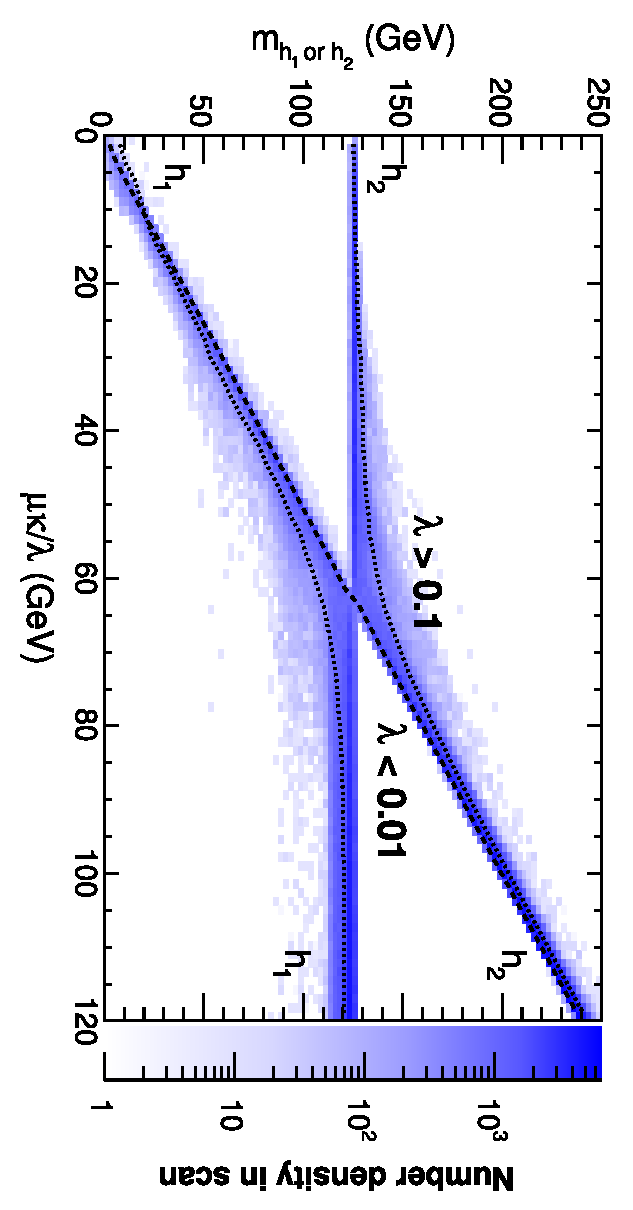
\includegraphics[height=0.48\linewidth, angle=90]{plots/newbranching/smass12_vs_mkovel.eps}
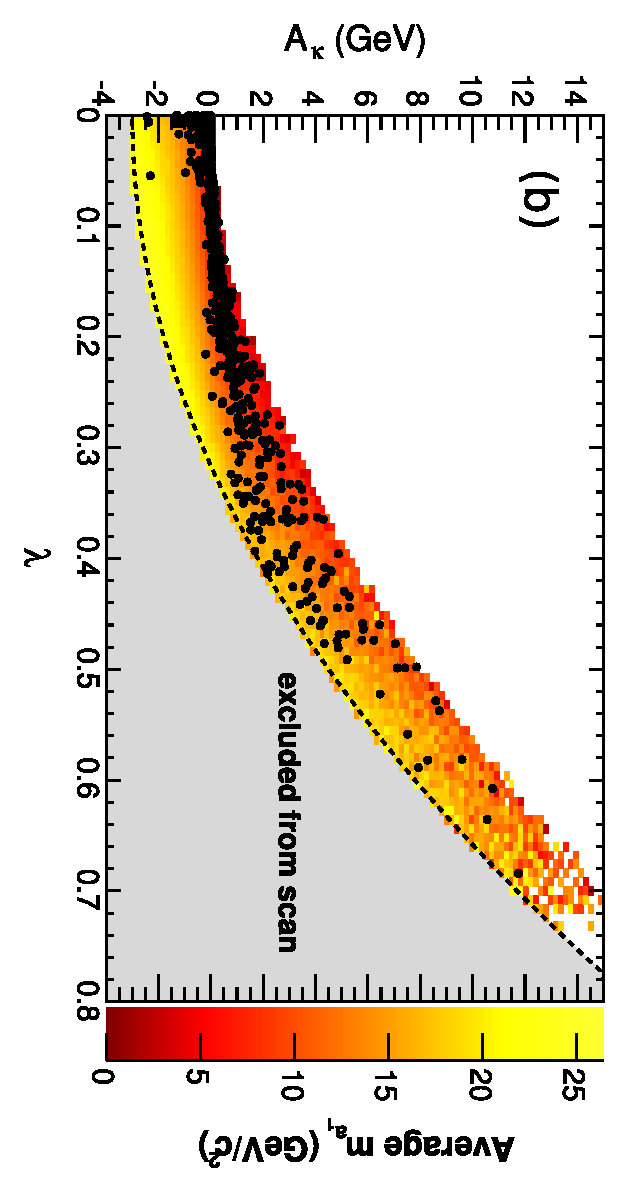
\includegraphics[height=0.48\linewidth, angle=90]{plots/newbranching/ma_vs_akappa_vs_lambda.eps}
\caption{Left: Lightest ($h_1$) and second-lightest ($h_2$) CP-even
  Higgs masses as a function of $\mu\kappa/\lambda$ and $\lambda$.
  The density of generated points surviving constraints is shown in
  the blue color scale, and the red line presents the single-valued
  $\lambda \ll 1$ limit.  Right: mass of the CP-odd Higgs ($m_a$) as a
  function of $A_\kappa$ and $\lambda$.  The color scale is the
  average mass in each bin, and filled circles are models with $m_a <
  2m_\tau$.  Low $m_a$ region follows the parabolic curve, $A_\kappa -
  (\mbox{30~GeV})\lambda^2 \ge 0$.
 \label{fig:hmass_mukoverl}}
\end{figure*}

For small  $\lambda$, $A_\lambda$ and $A_\kappa$, the $\CM_{S33}^2$ determines the mass 
of the lightest CP-even Higgs mass if $\kappa s = \mu\kappa/\lambda$ is small. In this 
case, $m_{h1}\simeq \sqrt{4\kappa s} = 2\mu\kappa/\lambda$. This relation is illustrated in 
Fig.~\ref{fig:hmass_mukoverl}(left) for $\kappa\mu/\lambda< 60$ GeV
when $h_1$ with $m_{h1}<120$ GeV has a significant singlet component,
especially for small values of $\lambda$ (and $A_\lambda$) when
the doublet-singlet mixing is suppressed. For larger values of $\kappa\mu/\lambda>60$ GeV,
$\CM_{S33}$ starts defining the mass of the $h_2$ Higgs boson with mass 
$m_{h2}\simeq  2\kappa\mu/\lambda$ and aquires a large singlet component, while $h_1$ 
becomes essentially the SM-like Higgs. In our scan we chose the upper bound on 
$\kappa\mu/\lambda<120$ GeV to create two equal size but phenomeologically distinct 
sub-regions.

The last parameter,  $A_\kappa -(\mbox{30~GeV})\lambda^2$, and its scan range
is motivated by the  shape of
the low $m_a$ domain shown in Fig.~\ref{fig:hmass_mukoverl}(right).
In this region $A_\kappa$ is limited to be small which is motivated
by RS limit, pushing $a_1$ to be light.
It selects a region with a roughly uniform distribution of light $m_a$ between 0 and 30~GeV
and removes most of the theoretically inaccessible region with $m_a^2<0$.  
%The phenomenology of $pp \to h_1 \to a_1a_1 \to 4\mu$ is determined 
%almost exclusively by the $\mu\kappa/\lambda$ ratio, $\lambda$, and 
%$A_\kappa$.  Varying $\tan\beta$ and $A_\lambda$ has negligible effect 
%on the masses, branching fractions, and production cross-section.


%In the $A_\kappa$-$\lambda$
%plane, $m_a$ grows with distance from a $A_\kappa =
%(\mbox{30~GeV})\lambda^2$ line, as seen in Fig.~\ref{fig:hmass_mukoverl}(right).
%The full dependence of $m_a$ can be approximately described by
%$\left[A_\kappa - (\mbox{30~GeV}) \lambda^2\right] \, \cdot \, \frac{\mu\kappa}{\lambda}
%\approx -(0.58 \, m_a)^2$ (true for 80\% of sampled points with at least 10\% accuracy).

\begin{figure*}[t]
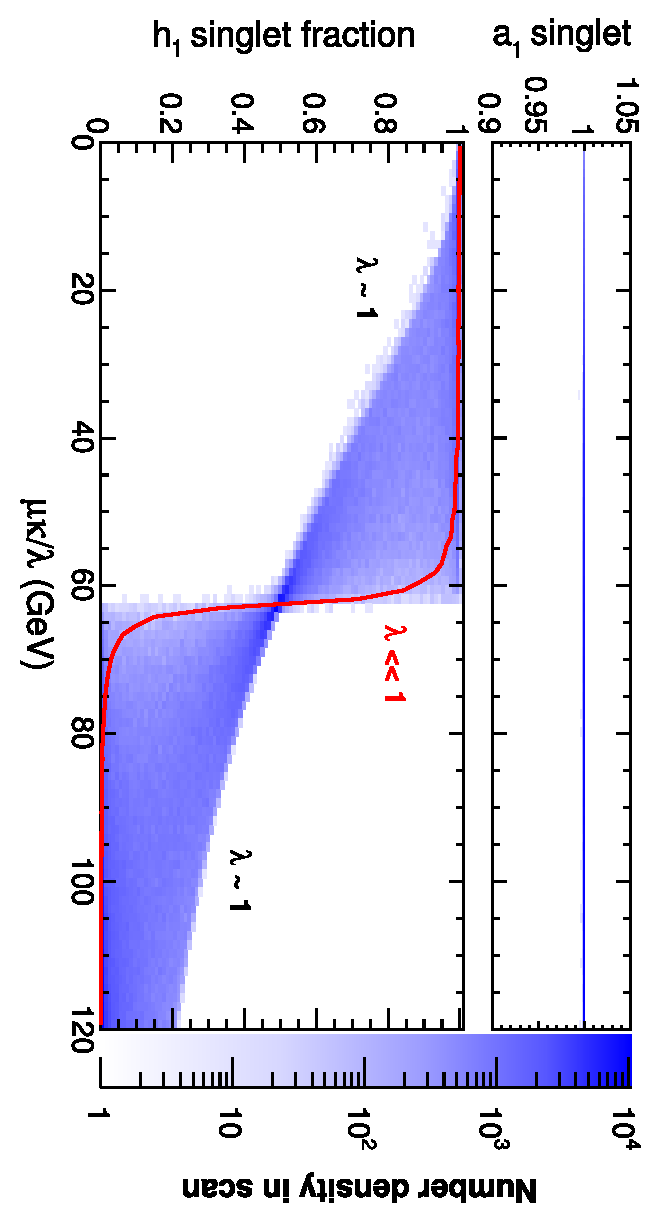
\includegraphics[height=0.50\linewidth, angle=90]{plots/newbranching/scomp13_vs_mkoverl.eps}
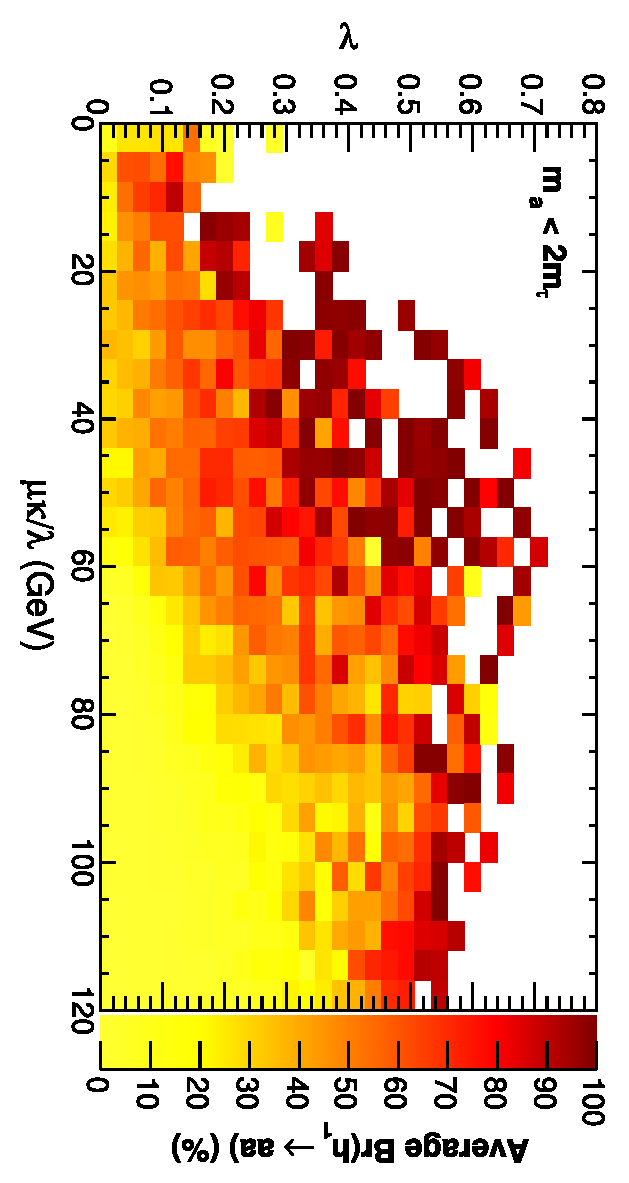
\includegraphics[height=0.46\linewidth, angle=90]{plots/newbranching/brhaa_vs_lambda_vs_mkoverl.eps}
\caption{Left: Singlet fraction of $h_1$ and $a_1$.  The singlet fraction of
  $a_1$ is nearly constant and approximately 1.0, while the singlet
  fraction of $h_1$ depends on $\mu\kappa/\lambda$ and $\lambda$. 
Right: Branching fraction of $h_1 \to a_1a_1$ in the $\lambda$, $\mu\kappa/\lambda$
  plane, with the requirement that $m_a < 2m_\tau$. \label{fig:singlet}}
\end{figure*}

The couplings of $h_1$ and $a$, to each other and to Standard Model
particles, are determined by their singlet and non-singlet componets.
One should notice, that in most of the  parameter space
$s=\mu/\lambda\gg v\sin 2\beta$, and, therefore, 
as one can see from Eq.(\ref{eq:pqmix},\ref{eq:rsmix}), 
the $s_{\theta_P}$ (which defines the signlet component of $a_1$)
is $\simeq 1$ in both, PQ and RS limits. 
Indeed, we have found, that
for the entire region of our interest, $a_1$ is close to a pure singlet 
(the non-singlet fraction $1-s_{\theta_P}^2  \lesssim 10^{-4}$)
but never is exactly a pure one.
The singlet fraction of $h_1$, $\SC_{13}^2$
is defined essentially by
$\mu\kappa/\lambda$ and $\lambda$,  as
illustrated in Fig.~\ref{fig:singlet}(left). 
Here we denote  $\SC_{13}$ as a mixing between the first ($H_{dR}$)
and  the third ($S_{R}$) CP-even Higgs boson weak eigensttaes.  
Increase of $\lambda$  enhances the  mixing of singlet and nonsinglet
Higgs boson eigenstates for both, CP-odd and CP-even Higgses.
\\
{\bf (let us plot  $\log(1-s_{\theta_P})$ versus $log( v \sin 2\beta \lambda/\mu)$,
 where v =174 GeV)}
 \\
 
For $\mu\kappa/\lambda \lesssim 60$~GeV, $h_1$ is predominantly a singlet 
(see Fig.~\ref{fig:singlet}(a) leading to a strong enhancement in the $h_1 aa$ coupling due 
to large singlet componets of both $h_1$ and $a_1$. Figure~\ref{fig:singlet}(b) shows the
enhancement in the corresponding branching ratio $Br(h_1\to a_1 a_1)$ for already 
small values of $\lambda$. For the same reason, the $h_1$ coupling to SM up or down- fermions 
is suppressed as ilustrated in Fig.~\ref{fig:sm_mukoverl1}(a). The corresponding suppression 
factors are determined by the elements of CP-even Higgs mixing matrix, 
$\SC_{11} = \sqrt{1-\SC_{13}^2-\SC_{12}^2}$ and $\SC_{12} = \sqrt{1-\SC_{13}^2-\SC_{11}^2})$, 
respectively. {\bf SOUNDS LIKE THE FOLLOWING IS PROBABLY NOT TRUE? One should note that $h_1$ coupling to 
$W$ and $Z$-bosons can be in general somewhat less suppressed} since it is proportional to combination 
{\bf TYPO IN THE FOLLOWING? of $\SC_{12}$ as $\SC_{11}$ as $(\sin\beta \SC_{12}+\cos\beta \SC_{11})$}, as 
illustrated in Fig.~\ref{fig:sm_mukoverl1}(b).
For $\mu\kappa/\lambda \gtrsim 60$~GeV, $h_1$ is a SM-like Higgs with only weak couplings to 
$a$ and respectively low branching ratio to $a_1a_1$ pairs, which can be somewhat enhanced
with large values of $\lambda$  softening the threshold between pure singlet and pure doublet,
see  Figs.~\ref{fig:singlet} and~\ref{fig:sm_mukoverl1}. In Fig.~\ref{fig:singlet}(b) which 
presents branching fraction of $h_1 \to aa$  as a function of $\mu\kappa/\lambda$ for models
with $m_a < 2m_\tau$ one can see that $Br(h_1 \to aa)$ remains large only when $\lambda$ is 
large, which is related {\bf DID YOU MEAN INCREASED SINGLET FRACTION AND LARGER COUPLING IN THE FOLLOWING? 
to the increased singlet fraction of $h_1$ together with the increased partial decay width $\Gamma(h_1 \to aa)$. 
A highly-singlet $h_1$ simultaneously has weak coupling to Standard Model 
particles (for both fermions and bosons, see Fig.~\ref{fig:sm_mukoverl1}) and, 
as long as $\lambda$ is not vanishingly small, has strong $h_1 aa$ coupling, 
so it decays to $aa$ with little competition from Standard Model modes.



\begin{figure*}[htbp]
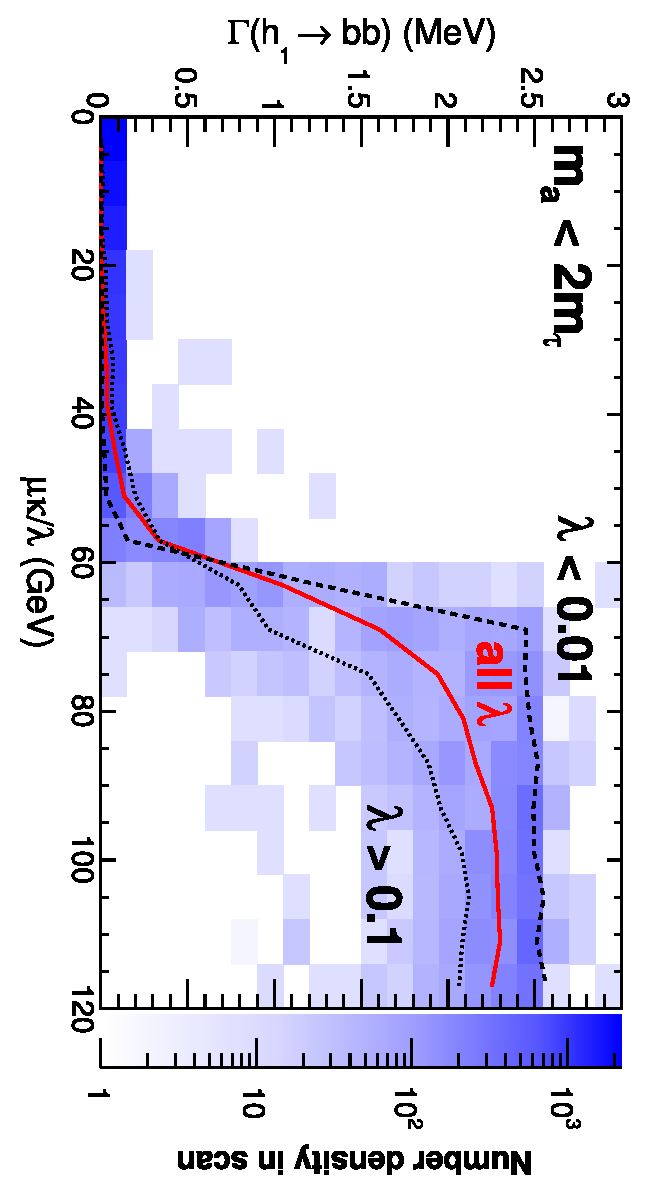
\includegraphics[height=0.56\linewidth, angle=90]{plots/newbranching/gammabb_vs_mkoverl.eps}%
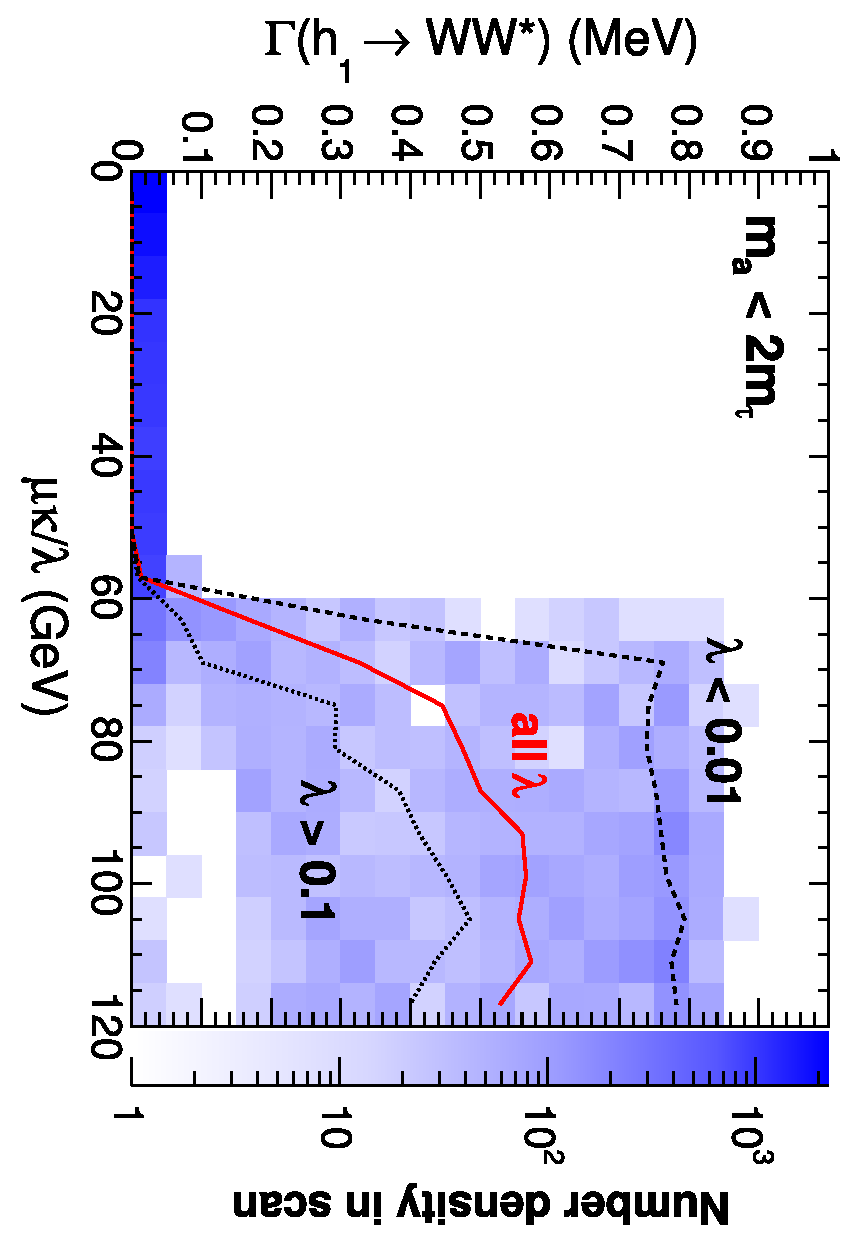
\includegraphics[height=0.44\linewidth, angle=90]{plots/newbranching/gammaww_vs_mkoverl.eps}
\caption{Partial widths of $h_1 \to b\bar{b}$ and $WW^*$ as a function
  of $\mu\kappa/\lambda$ and $\lambda$, with the requirement that $m_a
  < 2m_\tau$.  The red line presents the single-valued $\lambda \ll 1$
  limit {\bf (the plot on the right has not been correctly updated)}.
  {\bf TO BE REPLACED WITH REDUCED COUPLINGS FOR DOWN-TYPE FERMIONS
    AND BOSONS TO HELP ILLUSTRATE OUR LATER POINT ON LEP
    CONSTRAINTS. IF THEY ARE DIFFERENT FOR Z AND W (I DON'T THINK SO),
    CHOOSE THE HZZ COUPLING}
\label{fig:sm_mukoverl1}} \end{figure*}



\begin{figure*}[htbp]
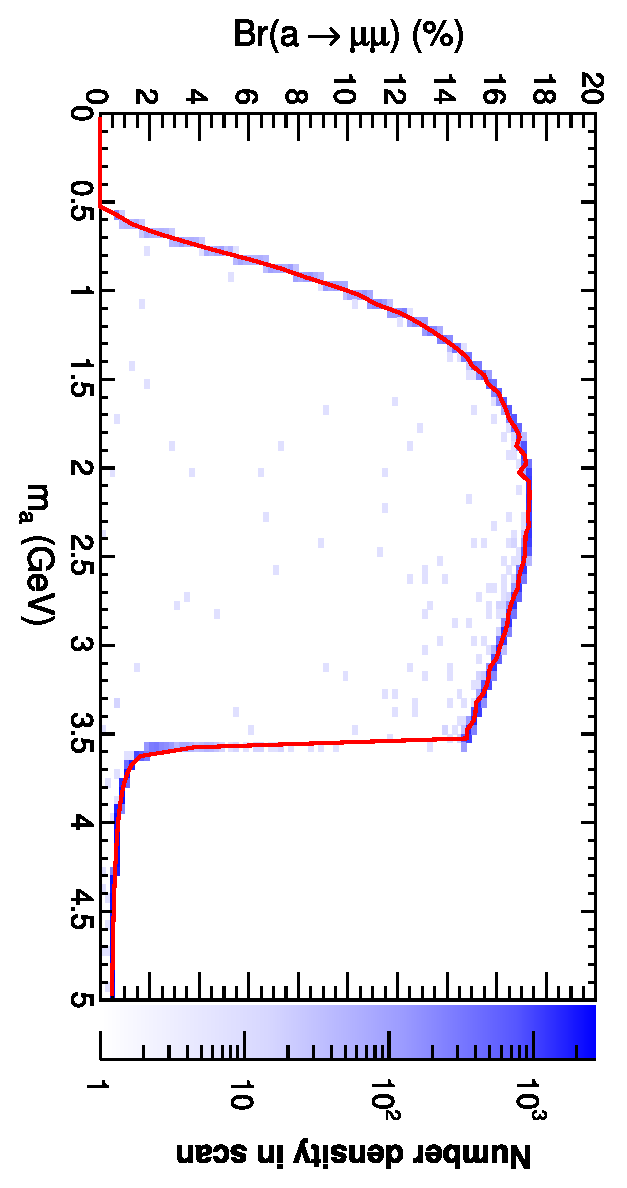
\includegraphics[height=0.54\linewidth, angle=90]{plots/newbranching/bra_vs_ma.eps}
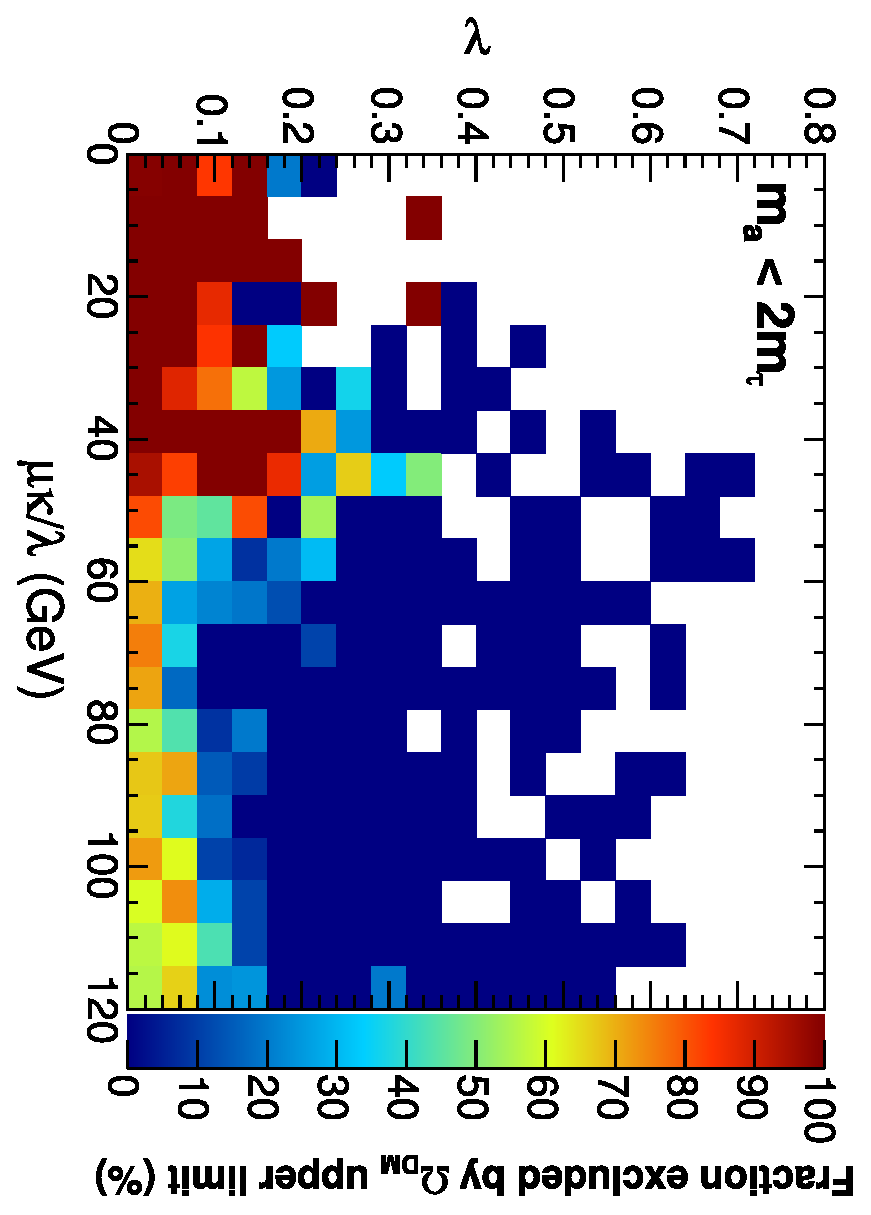
\includegraphics[height=0.42\linewidth, angle=90]{plots/newbranching/darkmatter.eps}
\caption{Left: Branching fraction of $a_1 \to \mu \mu$ for
  generated models as a function of $m_a$.  The red line is the average as a function of
  $m_a$, demonstrating that the branching fraction is nearly a strict
  function of mass.  The threshold at 3.55~GeV is $2m_\tau$. {\bf ADD SHADED RECTANGULAR TO COVER
THE REGION BELOW 0.5 SAYING THAT $a$ WILL HAVE LARGE BR TO MUONS IN THAT REGION AND REFER TO TEXT. 
WE ALSO NEED TO SAY THAT THE PAPER CITED BY D0 GIVES 27\% BR FOR MUONS. NEED SASHA TO LOOK INTO THIS. 
ALSO, WE ARE NOT GENERATING ANY POINTS BELOW 0.5 GEV B/C WE DID NOT TRY HARD ENOUGH. WE SHOULD BE 
ABLE TO GET THOSE BY CONSTRAINING THE SIXTH REQUIREMENT TO BE VERY SMALL NEGATIVE NUMBER. IT DOES 
NOT MEAN THAT NMSSMTOOLS WILL CORRECTLY CALCULATE BR RATIO THERE, BUT IT IS AN INTERESTING REGION, ISN'T IT?}  
Right: fraction of models with $m_a < 2m_\tau$ excluded by the WMAP dark matter constraint
as a function of $\lambda$ and $\mu\kappa/\lambda$. 
{\bf SECOND PLOT IS A CANDIDATE TO GO} \label{fig:brhaa}}
\end{figure*}

Because the coupling of a light nearly-singlet $a$ to all SM particles is strongly
but about equally suppressed, its branching fractions are not affected by the singlet
fraction of  $a_1$ and follow the standard mass hierarchy. Fig.~\ref{fig:brhaa}(a)
shows the the branching fraction for $a \to \mu\mu$ as obtained using NMSSMTools package. 
For $m_a < 2m_\tau$ the $a \to \mu\mu$ channel becomes significant, making an analysis
in the four muon mode viable for experimental searches. It is important to note that 
the calculation shown in Fig.~\ref{fig:brhaa}(a) was not meant tuned for $m_a<1$ GeV,
so some corrections are necessary. First, for $m_a<3m_\pi$, $B(a \to \mu\mu)$ is 
expected to be very high because $q\bar{q}$ and $gg$ decays are prohibited by hadronization 
and spin effects {\bf need a reference} and $\gamma \gamma$ is small {\bf (I just noticed 
that at m=1 GeV in the preprint with BR's we looked at, the sum of BR is ont 100\%?!!!!)}.
We compared predictions of NMSSMTools with (arXiv.0806.4411v2) and find a good agreement
between the two calculations, except that the (arXiv.0806.4411v2) the $B(\eta \to c \bar{c} )$,
obtained in the context of Little Higgs model and found to be dominant above $m_\eta=$2.5 GeV 
will be strongly suppressed in the context of NMSSM (the ratio of couplings of $a_1$ to up- 
and down-quarks is about $1-3 \times 10^{-3}$ for the parameters space applicable to our
study). {\bf NEEDS VERIFICATION: It is also worth noting that the recent paper by DZero
has used an incorrect B - I am not sure, I will check unless someone else can check that 
explicitly - Alexei}.

\subsubsection{Cosmological Constraints}

WMAP constraints on Cold Dark Matter (CDM) relic density can potentially be an
important constraint of NMSSM parameter space under study
where the CDM is lightest neutralino.
To restrict our scan to models consistent with experimental measurements of relic 
density, we used MicrOmegas package~\cite{micrOmegas} linked to NMSSMTools
dark matter  contribution $\Omega_{NMSSM}$ 
and required $\Omega_{NMSSM} \le 0.1099 + 2\times0.0062$,
which corresponds to the 95\% upper limits from the latest WMAP 5-year dataset. 

This WMAP bound  excludes the region of 
small $\mu\kappa/\lambda$ and $\lambda$ as shown in Fig.~\ref{fig:brhaa}(right)
where neutralino is being driven to be light and weakly interacting to SM
particles which suppress neutralino annihilation rate and respectively enhances 
neutralino relic density to unacceptably large values.


Figure~\ref{fig:exclusion}(a\&b)  show the density of models generated and those surviving WMAP 
constraints as a function of $\lambda$ and $\mu\kappa/\lambda$.

\subsubsection{Constraints from Direct Searches at Colliders}

Figure~\ref{fig:exclusion}-c shows the density of models surviving both WMAP and LEP constraints.
 LEP measurements exclude $h_1 \to aa$ within the kinematic
limits of $e^+e^- \to Z h_1$, $45 < m_{h_1} < 86$~GeV, and the
detector efficiency for light CP-odd Higgs bosons, $m_a > 2$~GeV
[ref].  Figure~\ref{fig:exclusion} presents
these experimental limits.
{\bf (Need more discussionhere, will do later)}.

\begin{figure*}[htbp]
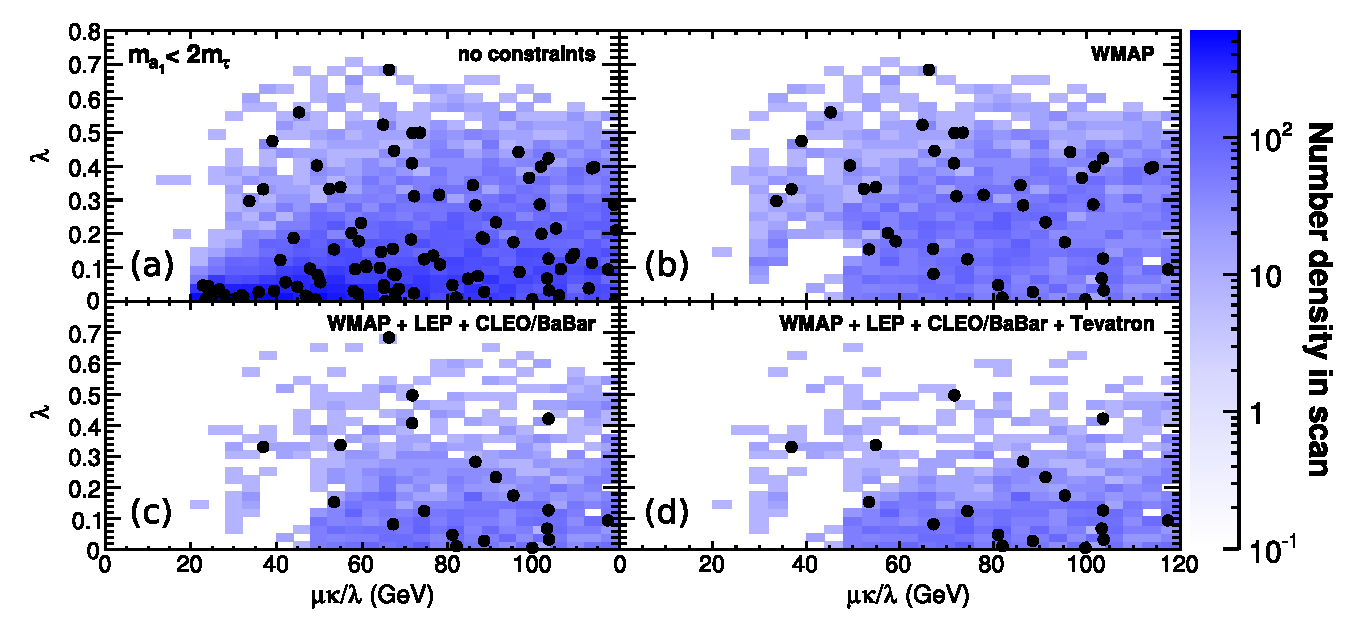
\includegraphics[height=0.48\linewidth, angle=90]{plots/newbranching/fourconstraints_params.eps}
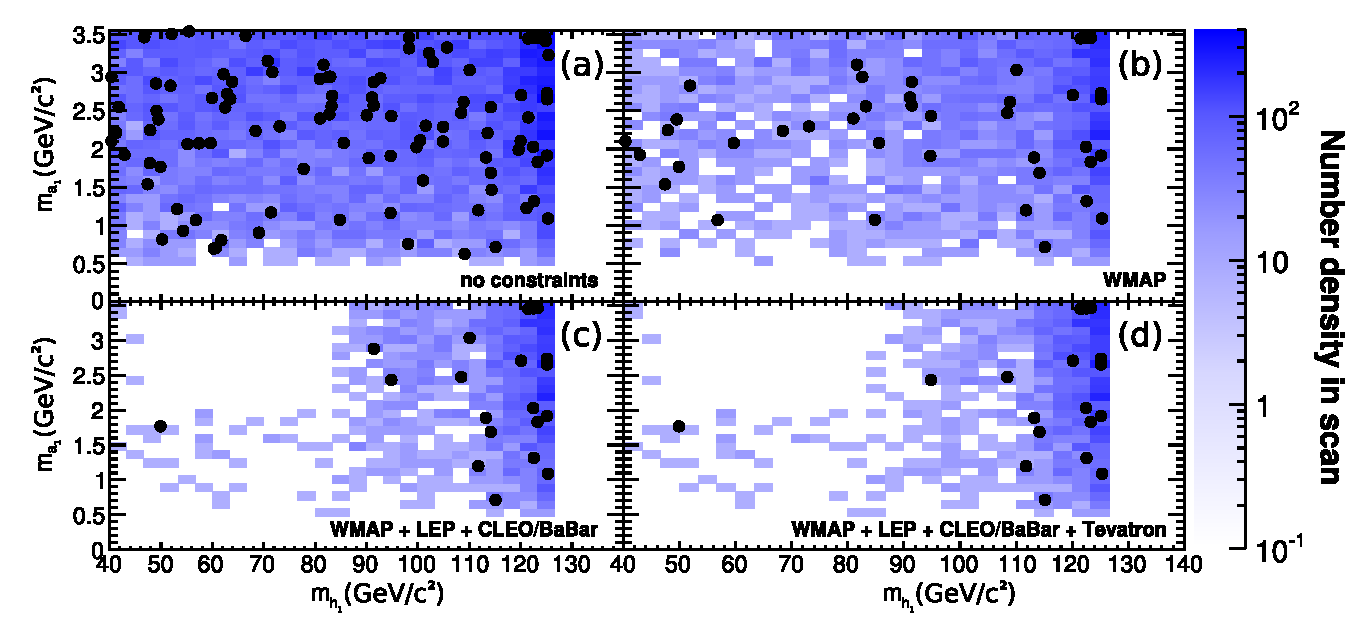
\includegraphics[height=0.48\linewidth, angle=90]{plots/newbranching/fourconstraints_masses.eps}
\caption{Sampled points with $m_a < 2m_\tau$ and experimental constraints successively applied.  Left: $\lambda$ vs.\ $\mu\kappa/\lambda$, right: $m_a$ vs.\ $m_h$.  Color scale is number density and filled points are 100 models (before application of experimental constraints). \label{fig:exclusion}}
\end{figure*}

In addition to LEP data, there have been several recent attempts aimed at direct searches. 
Searches at lower energy $e^+e^-$ colliders~\cite{cleo-low-ma,babar-low-ma} have been focusing on searching for the CP-odd Higgs 
via $\Upsilon \to \gamma a_1$ followed by $a_1$ decay to leptons. Neither of these searches can 
lead to any constraints on the NMSSM models with low $m_a$ because $a_1$ is always heavily dominated 
by singlet component (see the top plot in Fig.~\ref{fig:singlet}) and has absolutely negligible 
$bba_1$ coupling. {\bf (Is it sufficiently generic statement or is there smth specific in what we 
do other that asking for low $m_a$ that makes $a_1$ a singlet?)}. {\bf Did CLEO even look for such 
light mA? I thought they we looking for taus}. {\bf Our observations are confirmed by the results
obtained with the newest version of NMSSMTools.}

Another recent paper by $D\O$~\cite{d0-low-ma} describes the search for $a_1 a_1 \to \mu \mu \mu \mu$
using Tevatron data. To interpret the $D\O$ result, we calculate the NLO production cross-section for
$p \bar{p} \to h_1$ in NMSSM using the SM NLO calculations for $gg \to H_{SM}$~\cite{Spira:1995rr} and $b\bar{b} \to H_{SM}$
with QCD-improved (running) Yukawa couplings~\cite{Balazs:1998sb} corrected for differences in coupling between SM 
and NMSSM using the NMSSMTools:
\begin{eqnarray}
\sigma(gg\to h_1)=\sigma(gg\to H_{SM})\frac{\Gamma(h_1\to gg)}{\Gamma(H_{SM}\to gg)} \\ \nonumber
=\sigma(gg\to H_{SM})\frac{Br(h_1\to gg)\Gamma^{tot}(h_1)}{\Gamma(H_{SM}\to gg)} \\
\label{eq:ggcross_section} 
\sigma(b\bar{b}\to h_1)=\sigma(b\bar{b}\to H_{SM})
\left(\frac{Y_{bbh_1}}{Y_{bbH_{SM}}}\right)^2
\label{eq:bbcross_section} 
\end{eqnarray}
where $\sigma(gg\to H_{SM})$ and $\Gamma(H_{SM}\to gg)$ is calculated using
HIGLU, while $Br(h_1\to gg)$, $\Gamma^{tot}(h_1)$, and the ratio of Yukawa couplings 
$Y_{bbh_1}/Y_{bbH_{SM}}$ are obtained using NMSSMTools.

We select models for which 
$\sigma(p\bar{p} \to h_1) \times B_{h_1 \to aa \to 4\mu}$ does not exceed the upper limit of 
$\sigma_{95\%}=6$~fb obtained in~\cite{d0-low-ma}. {\bf BECAUSE 
PUBLISHED LIMIT MUST BE A FUNCTION OF h1 MASS, WE CORRECT $\sigma_{95\%}$ BY SCALING IT WITH $\alpha(m_{h1})/ \alpha_0$,
WHERE $\alpha_0$ is the acceptance given in ~\cite{d0-low-ma} 
for mass $m_{h1}=XXX$ and $\alpha(m_{h1}) = (m_{h1}/XXX) \times \alpha_0$
Sasha: let use different name for $\alpha$, it triggers $\alpha_S$ etc.}. 
Figure~\ref{fig:exclusion} shows the density of low $m_a$ models surviving WMAP, LEP and Tevatron constraints. 
It turns out that for $\mu\kappa/\lambda<60$ (non-SM $h_1$ lighter than 120 GeV), the cross-section 
is strongly suppressed even compared to SM for low $m_a$ because $h_1$ has a large singlet fraction. For 
larger $\mu\kappa/\lambda$ the lighest CP-even higgs $h_1$ becomes the SM-like Higgs and has negligible 
$h_1 \to aa$ branching.  These effects lead to the Tevatron data having only a very small impact on the allowed 
NMSSM parameter space. A significant improvement in Tevatron reach for NMSSM would have required a large increase 
in integrated luminosity likely leaving it up to LHC to make a definitive discovery or exclusion of
NMSSM models with low $m_a$.

%% \begin{figure*}
%% 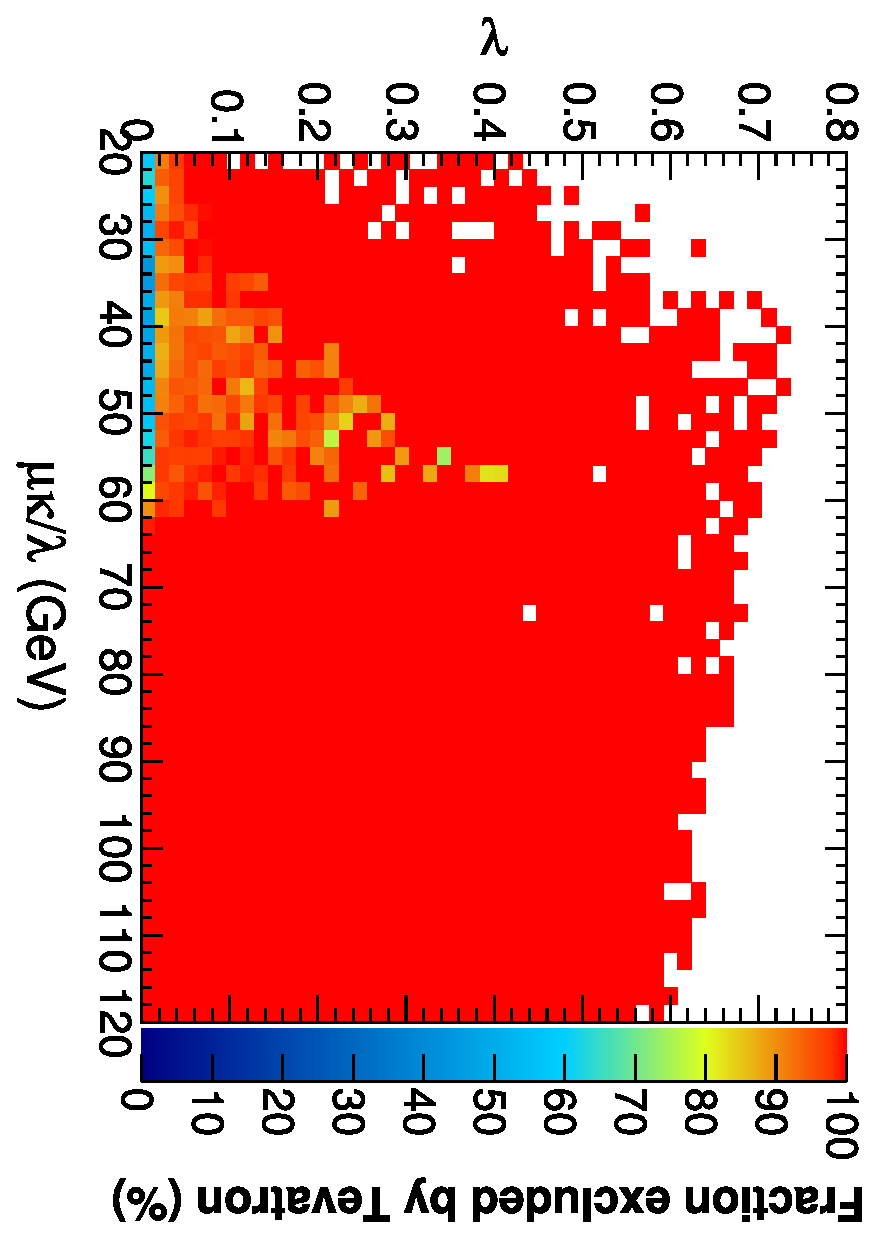
\includegraphics[height=0.45\linewidth, angle=90]{plots/newbranching/fraction_excluded_tevatron.eps}
%% 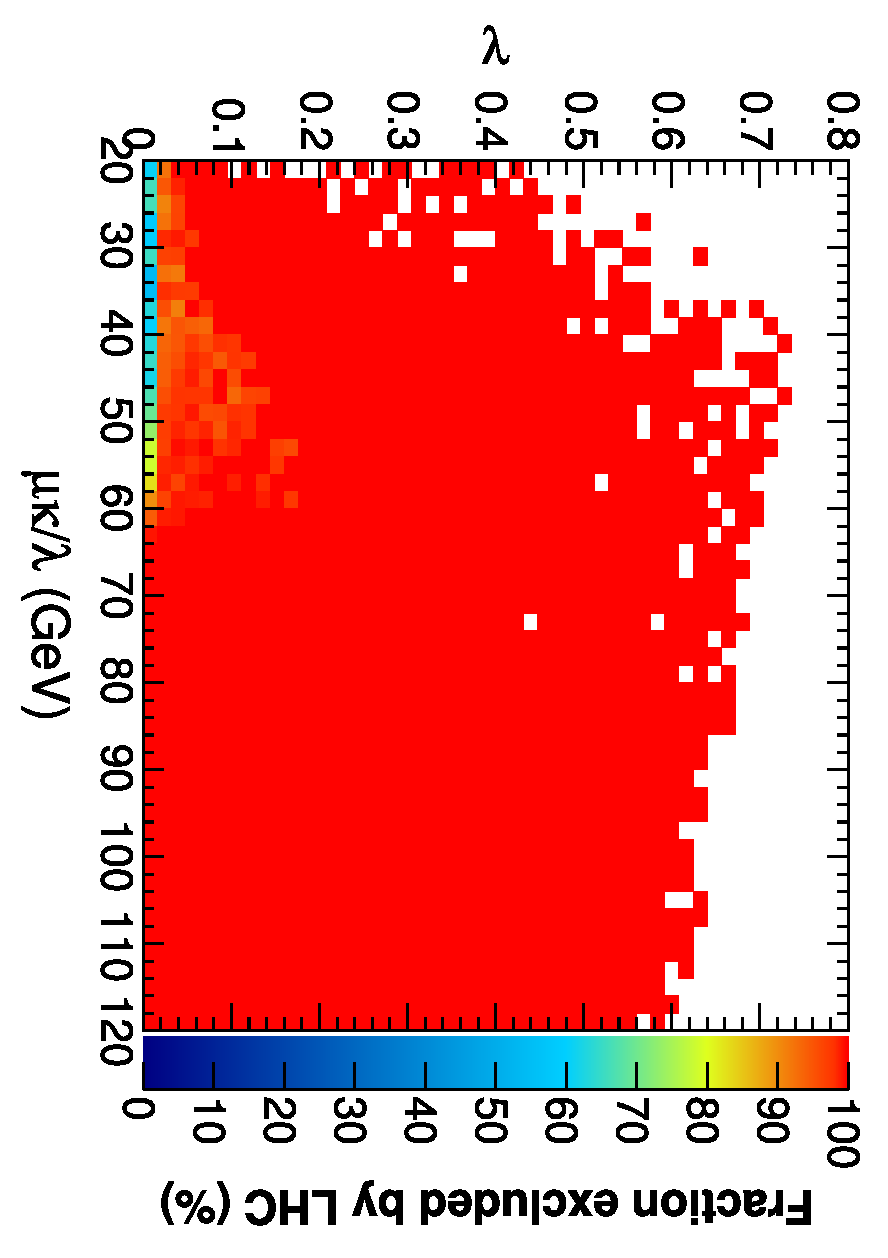
\includegraphics[height=0.45\linewidth, angle=90]{plots/newbranching/fraction_excluded_lhc.eps}
%% \caption{The fraction of generated models excluded by Tevatron and LHC
%%   limits (assuming $\mathcal{L}=100$~pb$^{-1}$ and 14~TeV: $\sigma(pp
%%   \to h_1 \to a_1a_1 \to 4\mu) < 100$~fb).  Red regions are excluded
%%   for all values of the other parameters.
%%  \label{fig:fraction_excluded}}
%% \end{figure*}

%% \begin{figure*}
%% 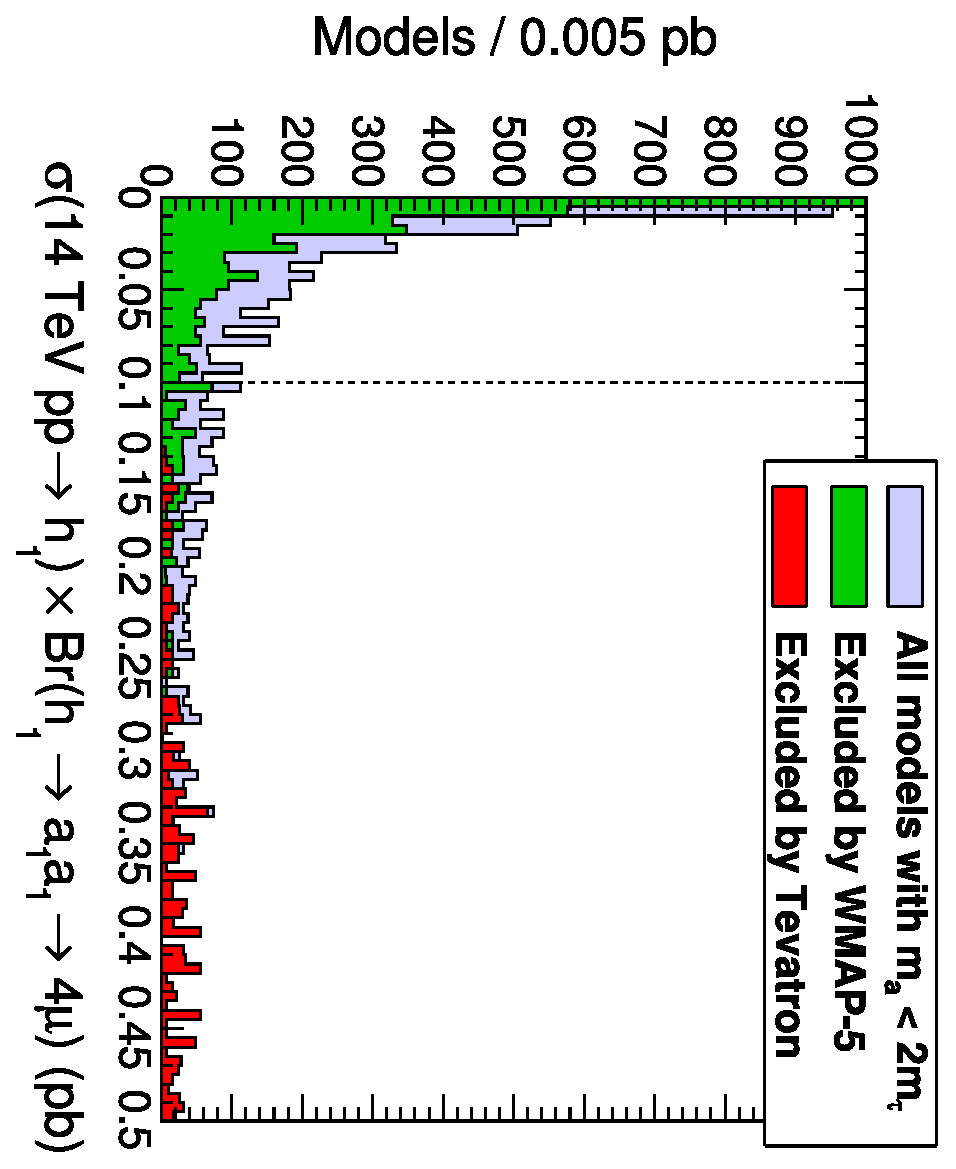
\includegraphics[height=0.45\linewidth, angle=90]{plots/newbranching/exclusion_1d.eps}
%% 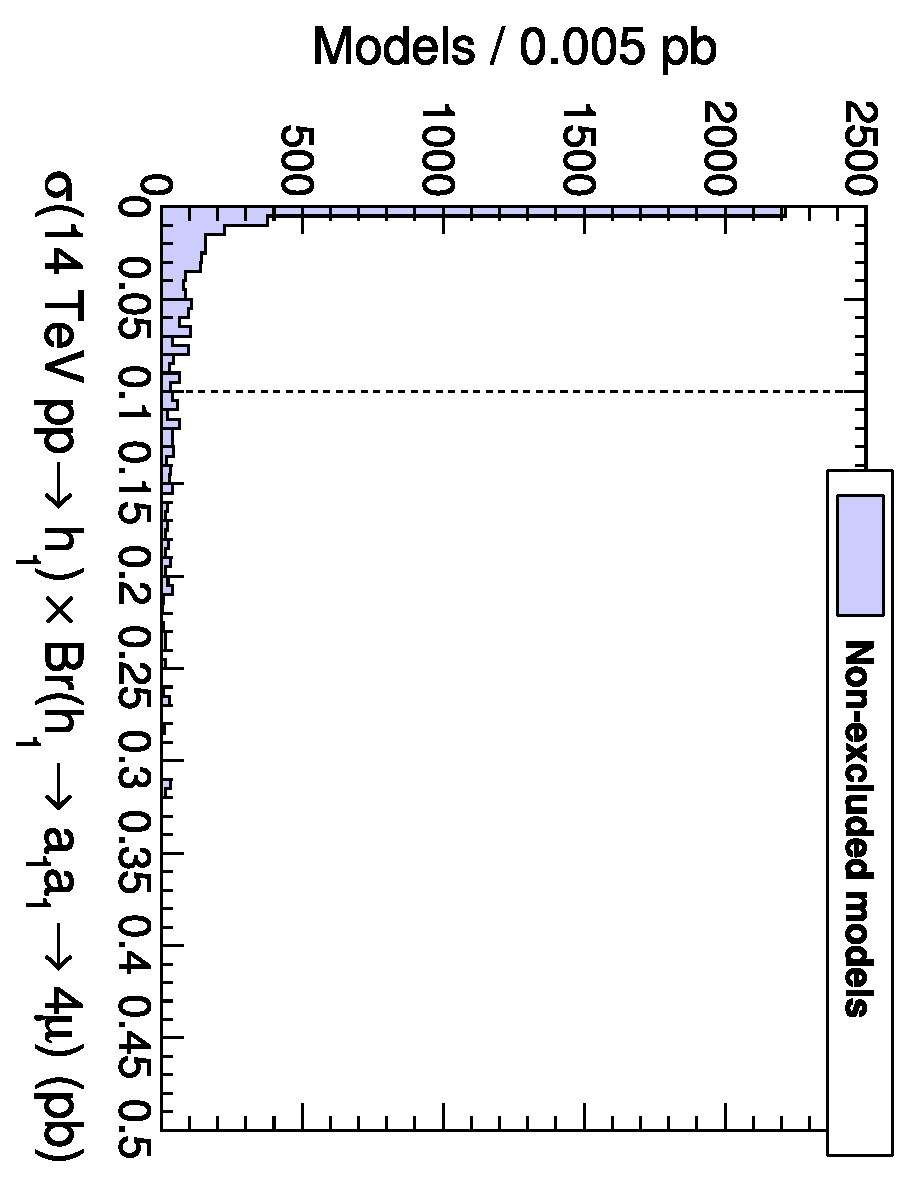
\includegraphics[height=0.45\linewidth, angle=90]{plots/newbranching/exclusion_1d_2.eps}
%% \caption{Left: generated models distributed by their effective LHC
%%   cross-section, with excluded models colored.  Right: a difference
%%   plot, showing only non-excluded models.  \label{fig:exclusion1d}}
%% \end{figure*}

%% We have  performed  two scans ``wide'' and ``narrow,'' 
%% where the narrow scan focuses more exclusively on the region
%% with dominant  $B_{h \to aa}$.\\
%% {\bf I do not observe a big difference between two scans
%%     which would make them called "wide" and "narrow".
%%     I believe that wide scan is too narrow, especially for $A_\kappa$
%%     which is  general in the hundreds of GeV range.}
%% Scans are uniform in each parameter listed in Table~\ref{brhaa_table},
%% subject to phenomenological and experimental constraints except for
%% the specialized LEP $h\to aa$ searches. 
%% \begin{table}[h]
%% \caption{Ranges for NMSSM parameter scans.  The narrow scan focuses on
%% the region with large $B_{h \to aa}$. \label{brhaa_table}}
%% \begin{center}
%% \renewcommand{\arraystretch}{1.2}
%% \begin{tabular}{| c c |}
%% \hline \mbox{\hspace{1.25 cm}}Wide scan\mbox{\hspace{1.25 cm}} & \mbox{\hspace{1.25 cm}}Narrow scan\mbox{\hspace{1.25 cm}} \\\hline
%% $0 < \kappa/\lambda < 0.8$ & $0 < \kappa/\lambda < 0.5$ \\
%% $0 < \lambda < 0.1$ & {\it same} \\
%% $-0.1 < A_\kappa < 0$~GeV & {\it same} \\
%% $0 < A_\lambda < 4$~TeV & $1 < A_\lambda < 3$~TeV \\
%% $100 < \mu < 200$~GeV & $100 < \mu < 150$~GeV \\
%% $10 < \tan\beta < 60$ & $10 < \tan\beta < 33$ \\\hline
%% \end{tabular}
%% \end{center}
%% \end{table}
%%  The $\lambda$ and $A_\kappa$
%% parameters are restricted even in the wide scan to yield small $m_a$
%% values, important for large $B_{a\to\mu\mu}$. 
%% In particular, we have restricted $A_\kappa$ to be in the really
%% narrow range motivated by the recent study~\cite{nmssm-ph7}.
%% Furthermore, in our study we have found that
%% important parameter for distinguishing between conventional Higgs
%% decays and  ${h \to aa}$ decays is the ratio of $\kappa$ over $\lambda$, so
%% we perform uniform scans in this ratio, rather than $\kappa$ alone.

%% Our first results of wide scan are presented in Fig~\ref{mass_exclusion}
%% which demonstrates quite know fact that in  allowed NMSSM parameter 
%% space two most probable scenarios the lightest CP-even Higgs boson 
%% take place.
%% In the first scenario the 
%% scalar Higgs is the SM-like,
%% obeys SM/MSSM LEP constraints~\cite{lep1exclusion,lep2exclusion}
%% to be above about 115 GeV
%% and  decays primarily into conventional $WW^*$, $b\bar{b}$,
%% and $\tau^+\tau^-$ modes 
%% as one can see from see Fig.~\ref{mass_exclusion}(right).

%% The other scenario
%% occurs when the lightest CP-even Higgs boson
%% has dominant singlet component, i.e. it is almost a singlet.
%% In this case, such a Higgs boson can be very light surviving
%% LEP constraints~\cite{lep1exclusion,lep2exclusion} 
%% and dominantly decays into the pair of CP-odd Higgs bosons $h_1\to a_1 a_1$
%% which are also have dominant singlet component.
%% Being an almost singlet in this scenario, lightest CP-even Higgs boson
%% interacts weakly with SM fermions and gauge bosons
%% and this allows it to escape LEP constrains even if its mass 
%% as low as 20 GeV. 
%% \\
%% {\bf Jim, could you please check if 
%% $h_1$ as light as 20 GeV survives from the scan?
%% Fig.1(left) shows that there are no 20 GeV $h_1$ survived.
%% I am not sure it is correct. Could you check, please
%% as well as check the Fig.1 caption?}
%% %


%% \begin{figure*}[htb]
%% \begin{center}
%% \includegraphics[width=0.5\linewidth]{plots/mass_exclusion.eps}%
%% 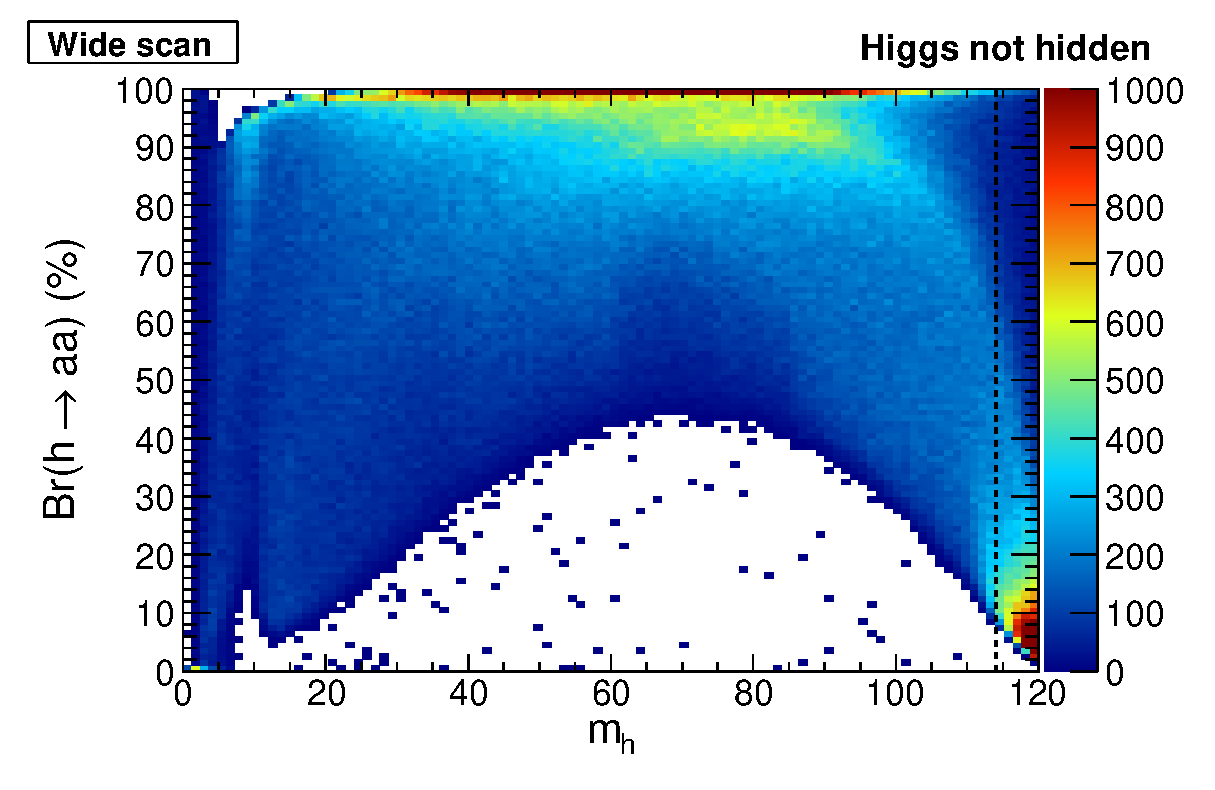
\includegraphics[width=0.5\linewidth]{plots/mh_brhaa.eps}
%% \caption{Left: regions of $m_a$ vs.\ $m_h$ excluded by LEP searches,
%%   right: the strong correlation between $m_h$ and $B_{h \to aa}$.  
%%   The above scan is subject to experimental constraints (other
%%   than the two specialized LEP searches for $h\to aa$) which require a
%%   conventionally-decaying Higgs to have $m_h >
%%   114$~GeV. \label{mass_exclusion}}
%% \end{center}
%% \end{figure*}


%% Fig~\ref{pmass1_Akappa} demonstrates the clear correlation between
%% $m_{a_1}$ and $\lambda$(left)
%% as well as 
%% $m_{a_1}$ and $A_{kappa}$(right)
%% in terms of density of randomly scattered points
%% ({\bf would also good to have plots for $m_{a_1}$ vs $\kappa/\lambda$
%%      since  $\kappa/\lambda$ is our principle parameter}).
%% We can see that if the mass of $a_1$ is  below its $\tau$ threshold decay 
%% then $\lambda$ is confined to be  below 0.1
%% while $A_\kappa$ is confined to be $|A_\kappa|<0.1$
%% ({\bf Jim, please,  check this statement from the wider scan}).
%% \begin{figure*}[htb]
%% \begin{center}
%% \includegraphics[width=0.5\linewidth]{plots/pmass1_lambda.eps}%
%% 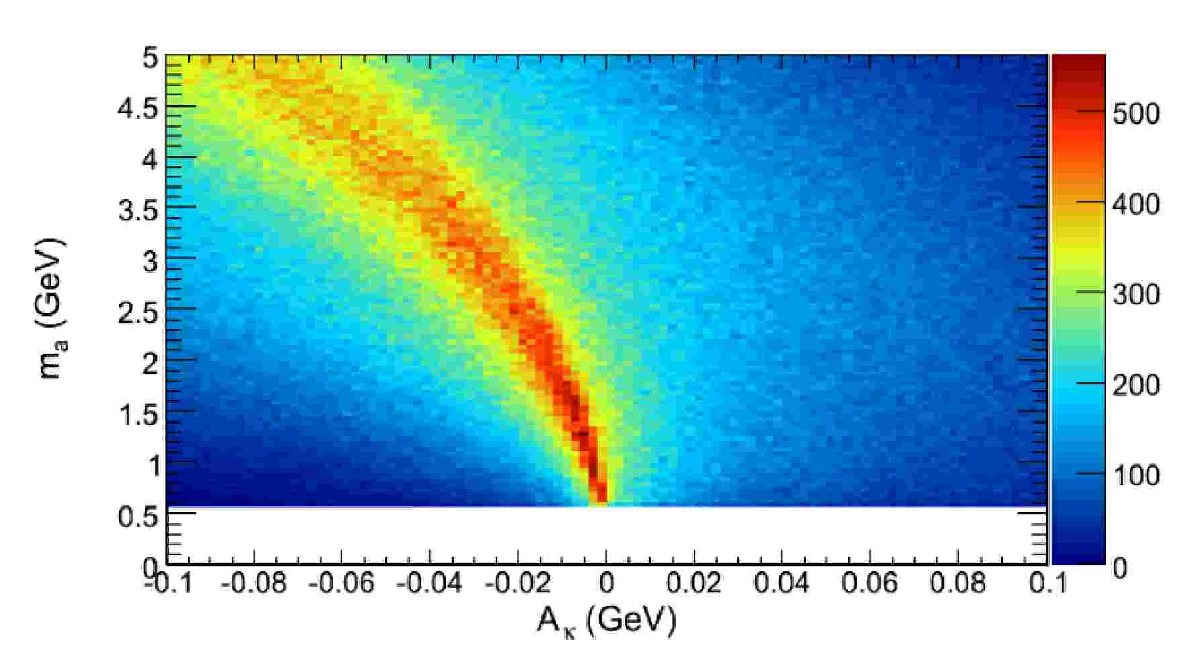
\includegraphics[width=0.5\linewidth]{plots/ma_vs_a-kappa.eps}

%% \caption{Both $\lambda$ and $A_\kappa$ must be close to zero for $m_a$
%%   to be below the $2 \, m_\tau$ threshold. \label{pmass1_Akappa}}
%% \end{center}
%% \end{figure*}

%% It is also essential to stress that $m_{a_1}<2m_\tau$
%% condition forces the lightest CP-odd Higgs $a_1$ to be
%% the singlet with very good accuracy. It's non-singlet admixture is
%% below 1\%, while for the lightest CP-even Higgs boson, $h_1$
%% two scenarios can be realized as mentioned above.
%% In Fig.~\ref{ma-vs-mh-vs-scomp}
%% we present the distribution of the admixture of the singlet component of  the
%% $h_1$ in the $m_{a_1}-m_{h_1}$ plane.

%% \begin{figure*}[htb]
%% \begin{center}
%% 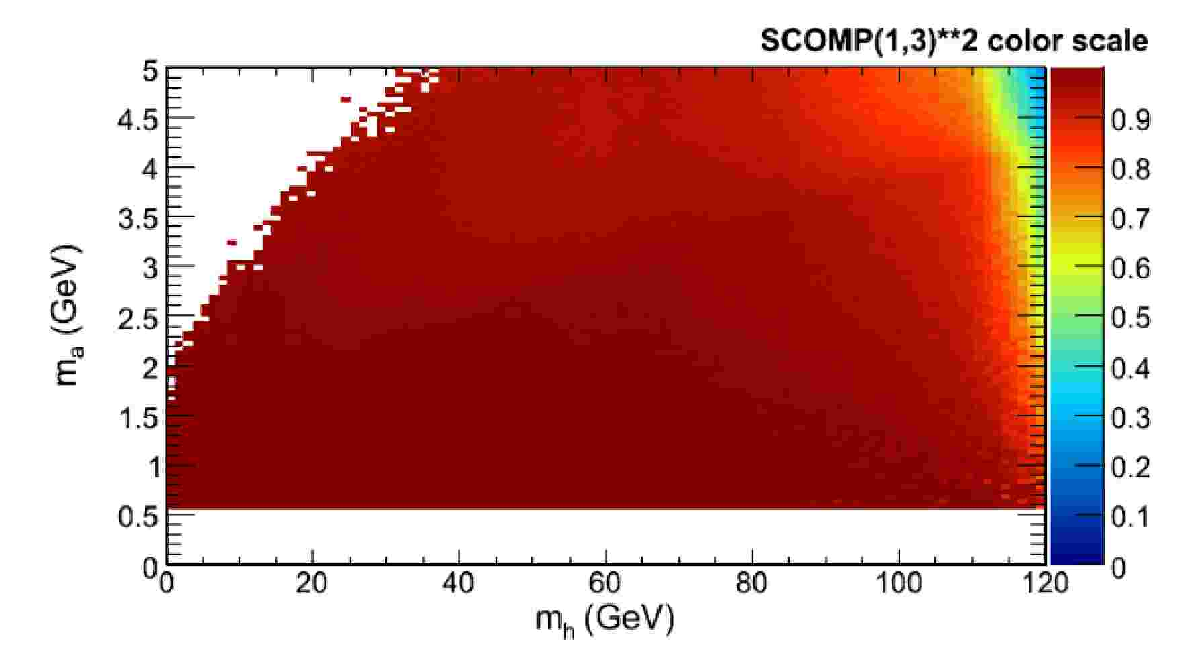
\includegraphics[width=0.75\linewidth]{plots/ma-vs-mh-vs-scomp.eps}
%% \caption{Distribution of the admixture of the singlet component of  the
%% $h_1$ in the $m_{a_1}-m_{h_1}$ plane
%% \label{ma-vs-mh-vs-scomp}}
%% \end{center}
%% \end{figure*}
%% One see that singlet component is dominated over the
%% whole parameter space subject of our scan except the region 
%% of the $m_{h_1}$ around 120 GeV when $h_1$ is essentially SM-like.
%% When the $h_1$ is essentially singlet, then role of the SM-like Higgs
%% is played by the next-to-lightest CP-even Higgs boson, $h_2$.
%% In Fig.~\ref{mh2-mh1-scomp} we illustrate this
%% presenting 
%% singlet and non-singlet admixture of $h_1$
%% in $m_{h_2}-m_{h_1}$ plane.
%% \begin{figure*}[htb]
%% \begin{center}
%% 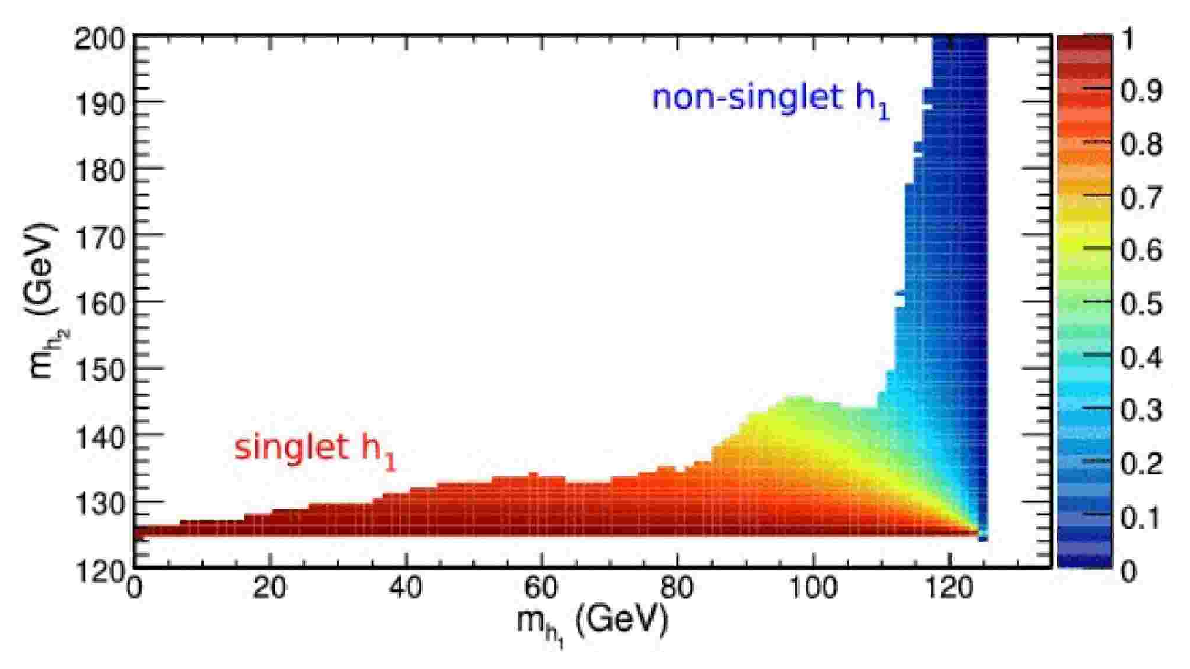
\includegraphics[width=0.75\linewidth]{plots/mh2-mh1-singlet.eps}
%% \caption{Singlet and non-singlet admixture of $h_1$
%% in $m_{h_2}-m_{h_1}$ plane
%% \label{mh2-mh1-scomp}}
%% \end{center}
%% \end{figure*}

%% %%%%%%%%%%%%%%%%%%%%%%%%%%%%%%%%%%%%%%%%%%%%%%%%%%%%%%%%%%%%%%%%%%%%%%
%% %%%%%%%%%%%%%%%%%%%%%%%%%%%%%%%%%%%%%%%%%%%%%%%%%%%%%%%%%%%%%%%%%%%%%%
%% \subsection{The $h_1$ and $a_1$ branching ratios}

%% Since $a_1$ is essentially singlet, the singlet admixture
%% of $h_1$ defines its coupling to $a_1$
%% and the respective branching ratio $Br(h_1\to a1 a_1)$
%% as illustrated in Fig.~\ref{scomp13-vs-br-h-aa}
%% which presents singlet component of $h_1$
%% (mixing angle squared of the $h_1$ and the pure singlet state,
%% which is given by \verb|SCOMP(1,3)|$^2$ parameter in NMSSM tools)
%% versus $Br(h_1\to a1 a_1)$. 

%% \begin{figure*}[htb]
%% \begin{center}
%% 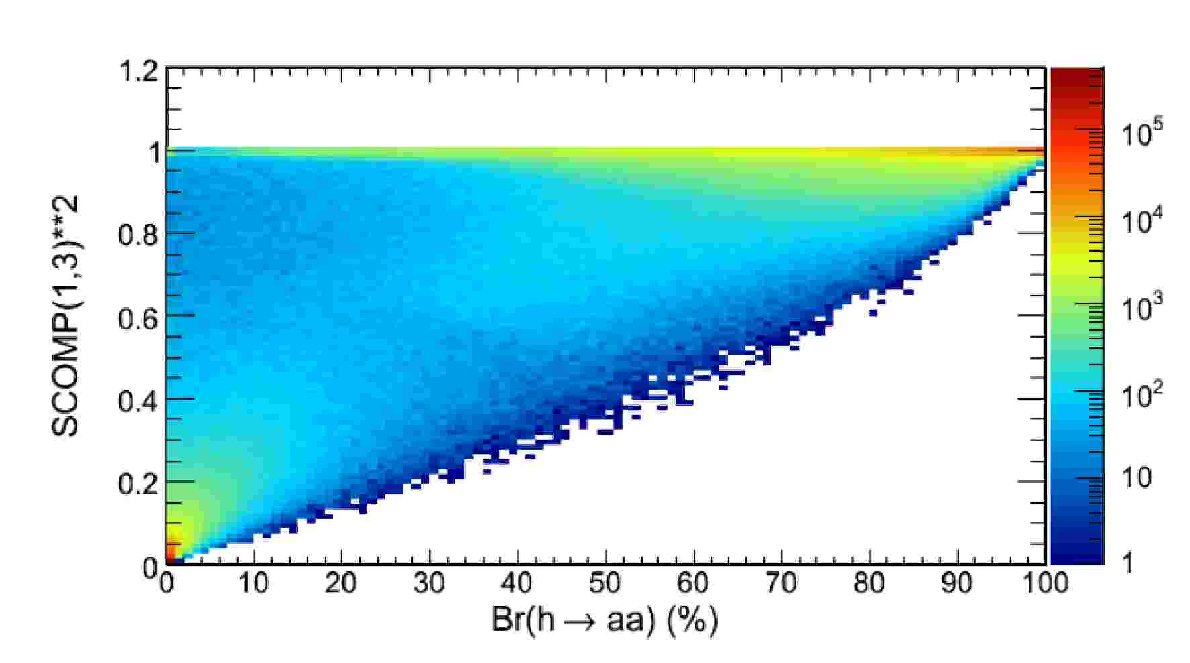
\includegraphics[width=0.75\linewidth]{plots/scomp13_vs_br_h-aa.eps}
%% \caption{Singlet component of $h_1$
%% (mixing angle squared of the $h_1$ and the pure singlet state)
%% versus $Br(h_1\to a1 a_1)$
%% \label{scomp13-vs-br-h-aa}}
%% \end{center}
%% \end{figure*}


%% The essential parameter which controls  the $h_1$ to be a
%% singlet or non-singlet we have found to be the ratio of
%% $\kappa/\lambda$  
%% ({\bf I think we need a plot scomp(1,3)$^2$
%% vs $\kappa/\lambda$  illustrating this}) 
%% which is eventually
%% controls  $Br(h_1\to a1 a_1)$ as demonstrated by $Br(h_1\to a1
%% a_1)$ vs  $\kappa/\lambda$ distribution in
%% Fig.~\ref{br-h-aa_vs_kap-lam}. One clearly see that for 
%% $\kappa/\lambda<0.3$, the $Br(h_1\to a1 a_1)$ is significant
%% which is related to the fact that the singlet component of
%% $h_1$ is large. One can see that the typical value of  
%% $Br(h_1\to a1 a_1)$ in this region is 70-100\%. 
%% ({\bf What are
%% competing Br of $h_1$ in this region?})




%% \begin{figure*}[htb]
%% \begin{center}
%% 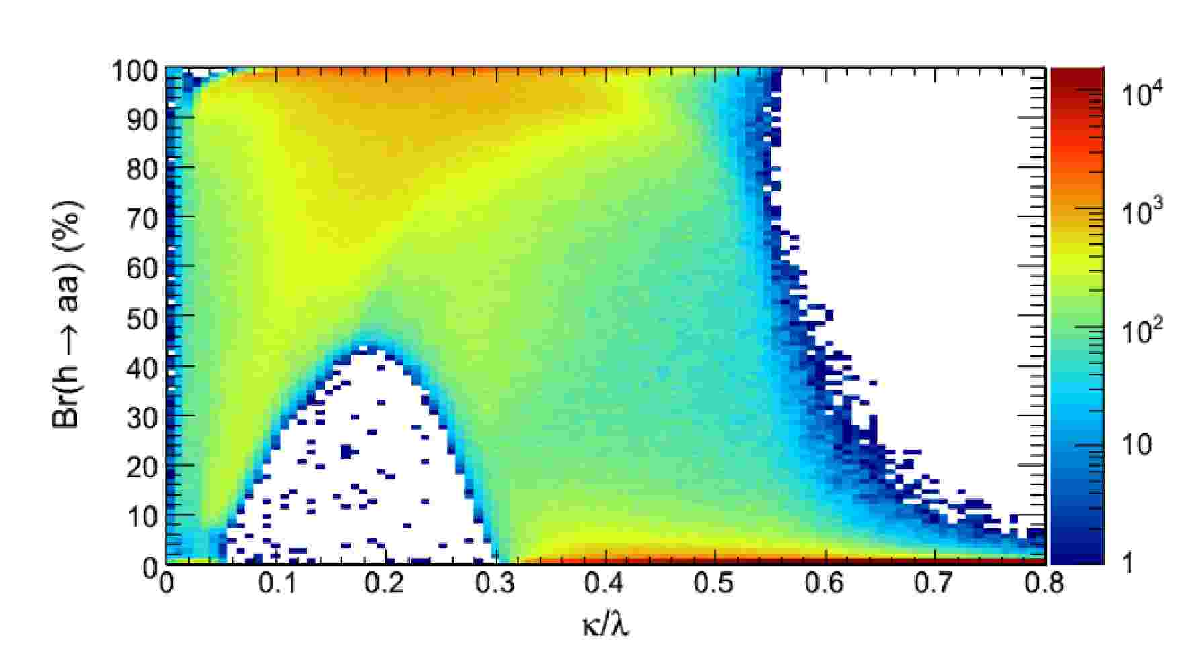
\includegraphics[width=0.75\linewidth]{plots/br-h-aa_vs_kap-lam.eps}
%% \caption{ $Br(h_1\to a1 a_1)$ vs  $\kappa/\lambda$
%% distribution.
%% \label{br-h-aa_vs_kap-lam}}
%% \end{center}
%% \end{figure*}
%% The singlet and non-singlet 
%% features of the lightest CP-even Higgs boson, $h_1$,
%% can be clearly disentangled in $\mu-\kappa/\lambda$
%% plane as one can see from Fig.\ref{mu-kaplam-scomp}.
%% For  $mu\simeq 110$~GeV,
%% $h_1$
%% becomes a singlet already for $\kappa/\lambda<0.5$ while for  $mu\simeq 200$~GeV
%% $h_1$ turns to be a singlet when $\kappa/\lambda<0.3$.
%% One can clearly see that $\mu$ and $\kappa/\lambda$
%% are essential variables defining the property of $h_1$
%% of being  singlet or non-singlet. 
%% ({\bf Why $\mu$ parameter was chosen in this narrow 100-200 GeV
%% range in our scan?\\
%%  One more remark/request: since  $\mu$ and $\kappa/\lambda$
%%  are very important parameters for the $h_1$, I would like to ask you to make
%%  plot
%% for the  color map of  $Br(h \to a_1 a_1)$
%%  in the same, ($\mu$-$\kappa/\lambda$) plane  -- this would be Fig.7b.
%%  })
%% \begin{figure*}[htb]
%% \begin{center}
%% 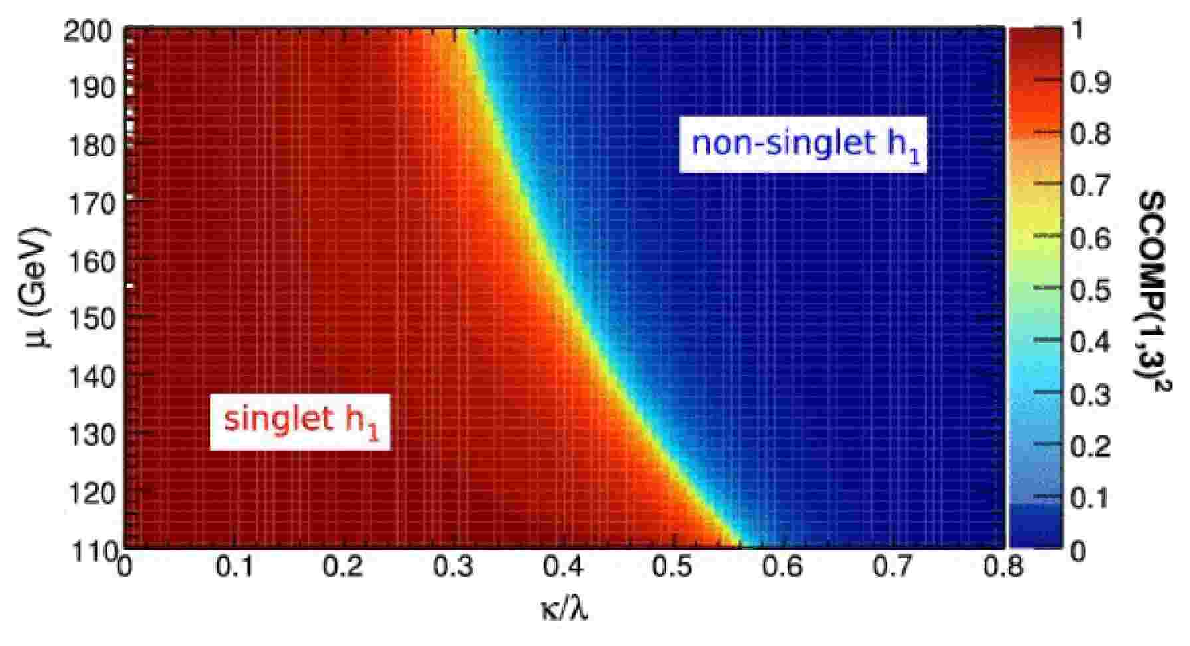
\includegraphics[width=0.75\linewidth]{plots/mu-kaplam-scomp.eps}
%% \caption{The singlet and non-singlet 
%% features of the lightest CP-even Higgs boson, $h_1$, 
%% in $\mu-\kappa/\lambda$
%% plane.
%% \label{mu-kaplam-scomp}}
%% \end{center}
%% \end{figure*}
%% Another representative plot  separating
%% singlet and non-singlet $h_1$ states
%% is the scatter plot of  the partial decay width $\Gamma(h_1\to a_1 a_1)$
%% versus  $\Gamma(h_1\to jj +bb+WW)$ shown in Fig.\ref{gh1-aa_vs_gh1-conv}.
%% The red and blue dots here denotes $h_1$ 
%% being 90\% singlet or 90\% non-singlet respectively.
%% ({\bf Did you include $h_1 \to \tau\tau$ ?})
%% One can see again how well  singlet/non-singlet states are separated
%% in the plane of these variables.
%% \begin{figure*}[htb]
%% \begin{center}
%% 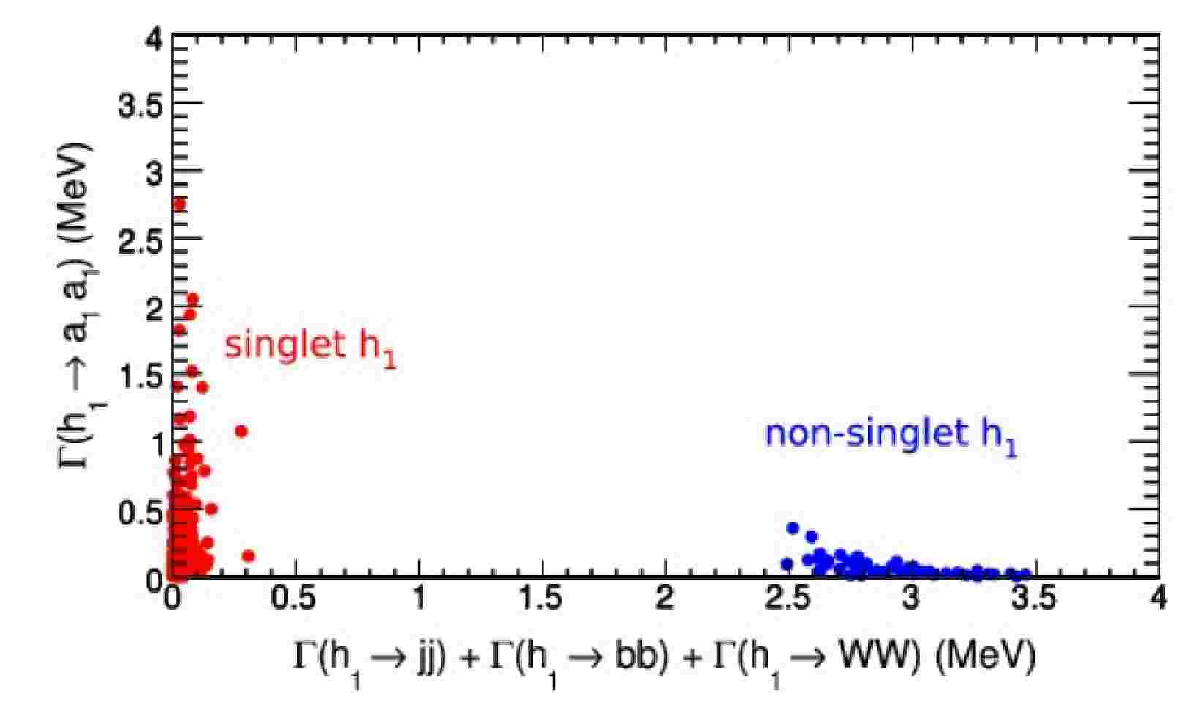
\includegraphics[width=0.75\linewidth]{plots/gh1-aa_vs_gh1-conv.eps}
%% \caption{Scatter plot of  the partial decay width $\Gamma(h_1\to a_1 a_1)$
%% versus  $\Gamma(h_1\to jj +bb+WW)$ .
%% The red and blue dots here denotes here that $h_1$ is
%% being 90\% singlet or 90\% non-singlet respectively.
%% \label{gh1-aa_vs_gh1-conv}}
%% \end{center}
%% \end{figure*}

%% As we have mentioned above,
%% $a1$ Higgs boson has extremely small non-singlet 
%% admixture  in the region of our interest
%% ($m_{a1} < 2m_\tau$),  however even though its non-singlet component is very smaill,
%% its branching ratio to $\mu^+\mu^-$ is large as soon as 
%% it kinematically allowed.
%% In Fig.\ref{pcomp13_vs_br_a-mm} (left) we present how large the  singlet
%% component of the light  $a_1$ can be  versus $Br(a_1\to\mu\mu)$.
%% In the Fig.\ref{pcomp13_vs_br_a-mm} (right) we show $m_{a1}$ distribution
%% in $\lambda-A_\kappa$ plain together with contour of the maximum value of 
%% $Br(a1\to \mu\mu)$ which is reached by at $m_{a1}\simeq 2$~GeV.
%% ({\bf I wanted to ask Jim the question about the meaning of the color.
%%      This point  should be clearly explained from the very beginning,
%%      when we start presenting plots like these.
%%      The question is the following: for each point(small area) in $\lambda-A_\kappa$
%%      plain we can have different values of $m_{a1}$. So, for the plot do you chose
%%      the max or min value of the  $m_{a1}$ for the color map?\\
%%      Another remark: eventually the left figure should be replotted in more 
%%      sensible way} )

%% \begin{figure*}[htb]
%% \begin{center}
%% 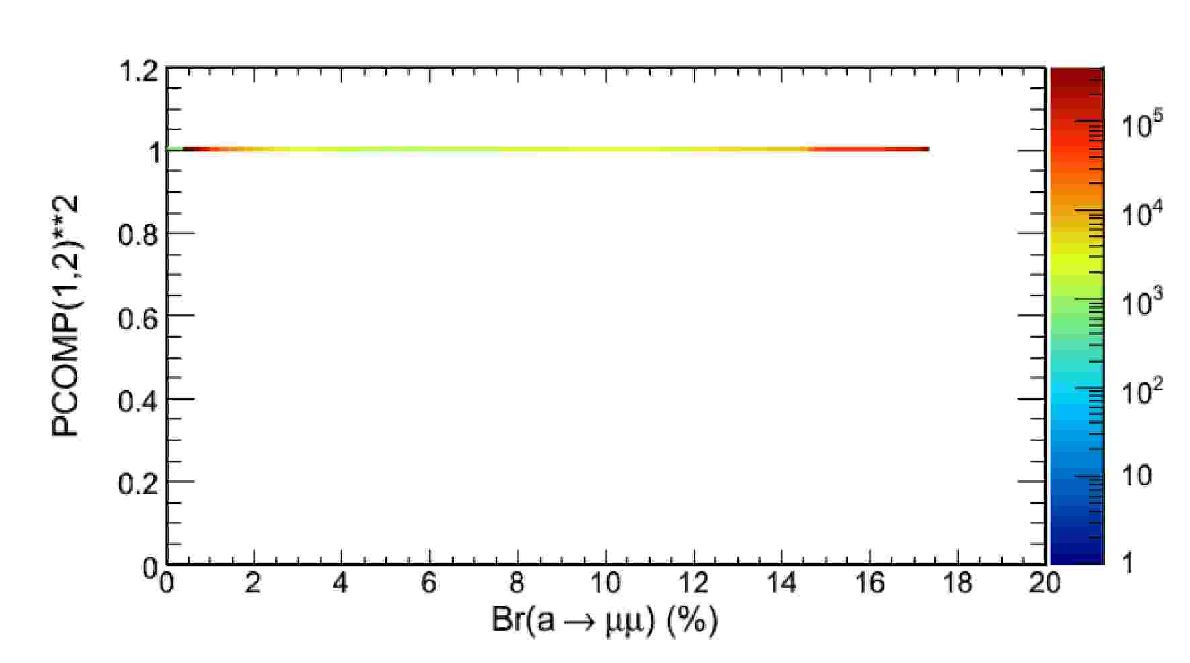
\includegraphics[width=0.5\linewidth]{plots/pcomp13_vs_br_a-mm.eps}%
%% 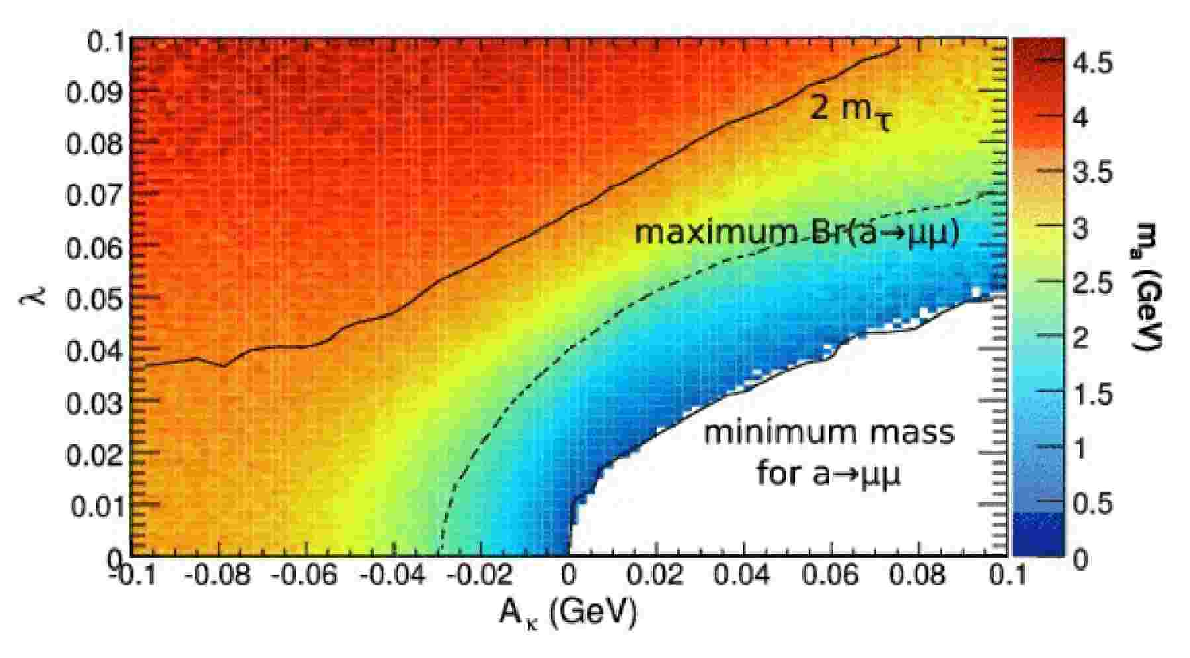
\includegraphics[width=0.5\linewidth]{plots/lam_vs_akap_ma.eps}
%% \caption{Left: the value of  singlet
%% component of the light  $a_1$ is versus $Br(a_1\to\mu\mu)$.
%% Right: $m_{a1}$ distribution
%% in $\lambda-A_\kappa$ plain together with contour of the maximum value of
%% $Br(a1\to \mu\mu)$ (dashed contour) 
%% which depends only on the kinematics defined by the $m_{a1}$.
%% \label{pcomp13_vs_br_a-mm}}
%% \end{center}
%% \end{figure*}

%% In Fig.~\ref{br-h-aa_vs_ma} we present the  value 
%% of  $Br(a_1\to\mu\mu)$ versus $m_{a1}$ which
%% we have tabulated and use in our analysis. 
%% It is important to stress that for a given $m_{a1}$
%% the value of  $Br(a_1\to\mu\mu)$ is essentially fixed
%% and is practically independent off other model parameters.
%% ({\bf We need more details on 
%% how this  Br is independent off other parameters
%% and how large deviations 
%% from the red curve can be. We should probably have
%% one more additional figure on this}).
%% \begin{figure*}[htb]
%% 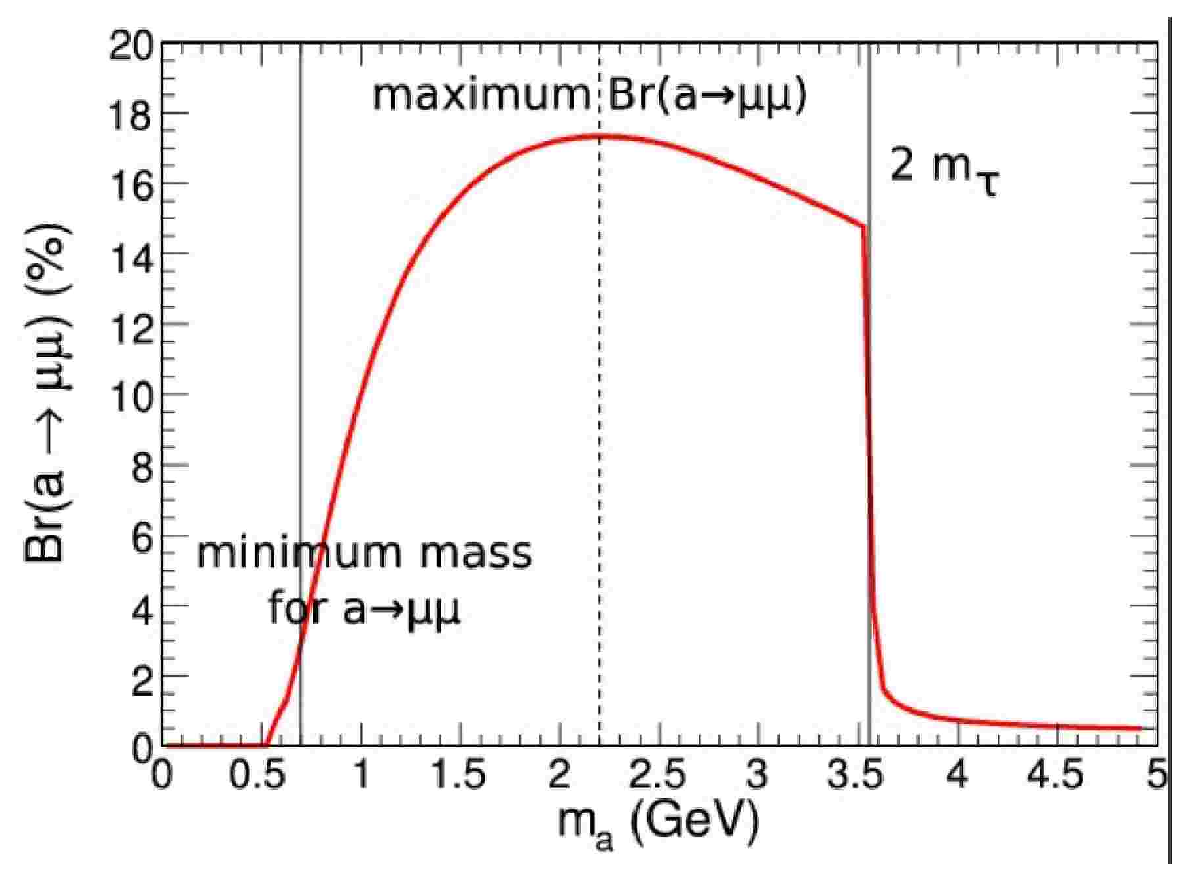
\includegraphics[width=0.75\linewidth]{plots/br-h-aa_vs_ma.eps}%
%% \caption{The  value 
%% of maximal  $Br(a_1\to\mu\mu)$ versus $m_{a1}$ 
%% \label{br-h-aa_vs_ma}}
%% \end{figure*}
%% We can see that $Br(a_1\to\mu\mu)$ can be as large as 18\%
%% for $m_{a1}$ around 2 GeV.
%% In the mass
%% range of interest (below the $a \to \tau^+\tau^-$ threshold), the main
%% competing channels are $a \to gg$ and $a \to s\bar{s}$.


%% %%%%%%%%%%%%%%%%%%%%%%%%%%%%%%%%%%%%%%%%%%%%%%%%%%%%%%%%%%%%%%%%%%%%%%
%% %%%%%%%%%%%%%%%%%%%%%%%%%%%%%%%%%%%%%%%%%%%%%%%%%%%%%%%%%%%%%%%%%%%%%%
%% \subsection{Production rates}

%% As we have shown,
%% the lightest CP-even Higgs boson, $h_1$,
%% typically has significant singlet component
%% in the region of our  interest 
%% (i.e. in the region of $m_{a1}<2 m_{\tau}$) 
%% and as we have found above,
%% both, $Br(h_1\to a_1 a_1)$  and $Br(a_1\to \mu\mu)$,
%% are quite significant. In the same time,
%% one should expect the suppression
%% of the $h_1$ production rate since $h_1$ interacts weakly with the 
%% fermions and gauge bosons  due to its  singlet nature.

%% In our study we have evaluated $pp\to h_1$ production cross section
%% for the $gg\to h_1$ and $b\bar{b}\to h_1$ process
%% at the next-to-leading order (NLO)
%% using the following 
%% procedure.

%% First, we have used  
%% HIGLU v2.102 package~\cite{Spira:1995rr} to calculate 
%% SM Higgs production cross section in $gg\to H_{SM}$ process.
%% Since the ratio of  $\sigma(gg\to h_1)/\sigma(gg\to H_{SM})$
%% production cross sections is equal to the ratio
%% of partial decay widths $\Gamma(h_1\to gg)/\Gamma(H_{SM}\to gg)$, one finds
%% \begin{equation}
%% \sigma(gg\to h_1)=\sigma(gg\to H_{SM})\frac{\Gamma(h_1\to gg)}{\Gamma(H_{SM}\to gg)}
%% =\sigma(gg\to H_{SM})\frac{Br(h_1\to gg)\Gamma^{tot}(h_1)}{\Gamma(H_{SM}\to gg)}.
%% \end{equation}
%% Therefore we have all components to evaluate $\sigma(gg\to h_1)$:
%% we use
%% $\sigma(gg\to H_{SM})$ and $\Gamma(H_{SM}\to gg)$ calculated  using HIGLU at  NLO,
%% while $Br(h_1\to gg)$ and $\Gamma^{tot}(h_1)$ we obtain using NMSSMtools.


%% \begin{figure*}[htb]
%% 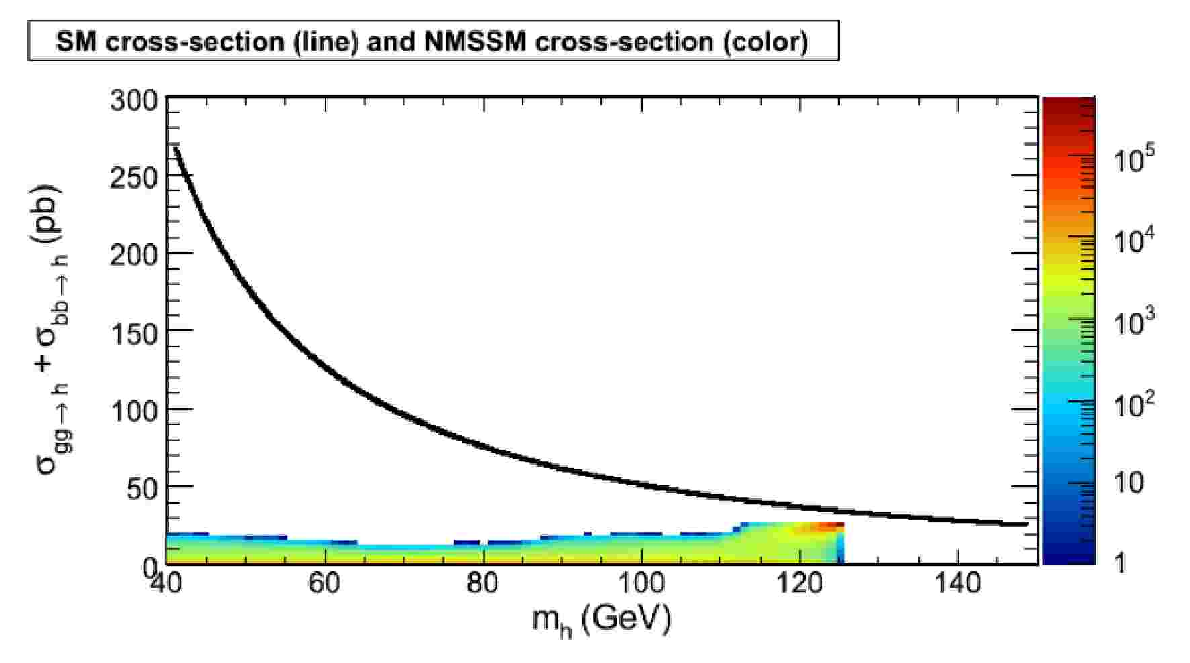
\includegraphics[width=0.5\linewidth]{plots/cs3.eps}%
%% 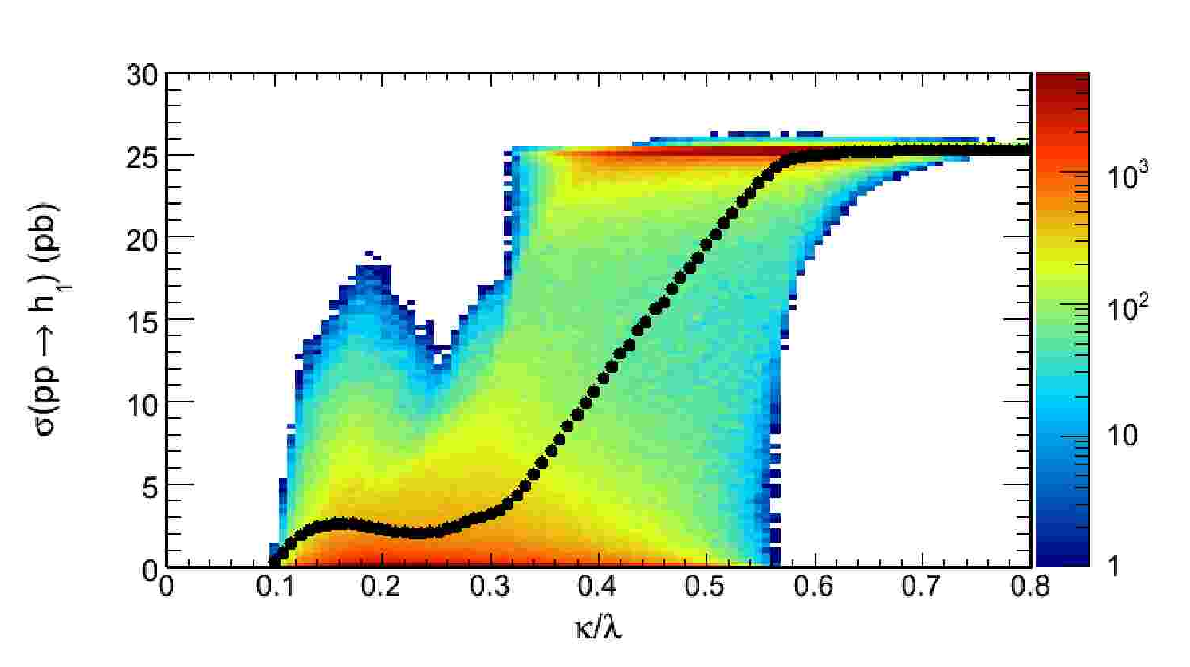
\includegraphics[width=0.5\linewidth]{plots/sig_vs_kaplam.eps}%
%% \caption{Combined 
%% $\sigma(gg\to {\cal H}) + \sigma(b\bar{b}\to {\cal H})$ production cross section
%% versus $m_{\cal H}$ for NMSSM and SM,
%% where ${\cal H}$ stands either for NMSSM or SM Higgs boson.
%% \label{cs3}}
%% \end{figure*}

%% The cross section of $b\bar{b}\to h_1$ was also evaluated at
%% NLO as follows. The numerical calculation for the  SM Higgs
%% production in  $b\bar{b}\to H_{SM}$ fusion has been carried out
%% with the program developed in \cite{Balazs:1998sb} and lately
%% used also in \cite{Belyaev:2005nu} where the QCD-improved
%% (running) Yukawa couplings have been used. Then using
%% $Y_{bbh_1}/Y_{bbH_{SM}}$ ratio of  Yukawa couplings 
%% calculated  in NMSSMtools, one finds:
%% \begin{equation}
%% \sigma(b\bar{b}\to h_1)=\sigma(b\bar{b}\to H_{SM})
%% \left(\frac{Y_{bbh_1}}{Y_{bbH_{SM}}}\right)^2
%% \end{equation}
%% For the evaluation of production cross sections, CTEQ6M set for
%% parton density function set was used. 

%% Our first results  on the
%% combined  $\sigma(gg\to {\cal H}) + \sigma(b\bar{b}\to {\cal
%% H})$ production cross section versus $m_{\cal H}$ for NMSSM and
%% SM  are presented in Fig.\ref{cs3} (left), where ${\cal H}$ stands
%% either for NMSSM or SM Higgs boson. 
%% The right frame of Fig.\ref{cs3} 
%% presents $\sigma(gg\to {\cal H}) + \sigma(b\bar{b}\to {\cal
%% H})$ versus $\kappa/\lambda$ for NMSSM in more details. 
%% ({\bf Can we present(or
%% think about how to present) also results for $\sigma(gg\to
%% {\cal H})$ $\sigma(b\bar{b}\to {\cal H})$ separately to show
%% their relative contribution? }).
%% From Fig.~\ref{cs3} we can see that 
%% production cross section of NMSSM $h_1$ is indeed
%% suppressed typically by 2 orders of magnitude as compared to the
%% SM Higgs boson production in case when 
%% $h_1$ has a significant singlet component. The value of the
%% minimal suppression depends on the mass of $h_1$:
%% for $m_{h1}\simeq 40-50$ GeV, the maximal cross section of $h_1$
%% production is about 10 smaller than the SM one, while
%% when  $m_{h1}\simeq 115-125$ GeV its production cross section
%% is quite close to SM and can be as large as about 25 pb 
%% once the singlet component of $h_1$
%% vanishes.

%% Since we study the whole production and decay chain
%% $pp\to h_1 \to a_1 a_1\to 4\mu$ let us  look at the
%% cross section of the four-muon production after application
%% of the respective branching ratios from NMMStoos
%% to the $h_1$ production cross section which we have evaluated.

%% \begin{figure*}[h]
%% 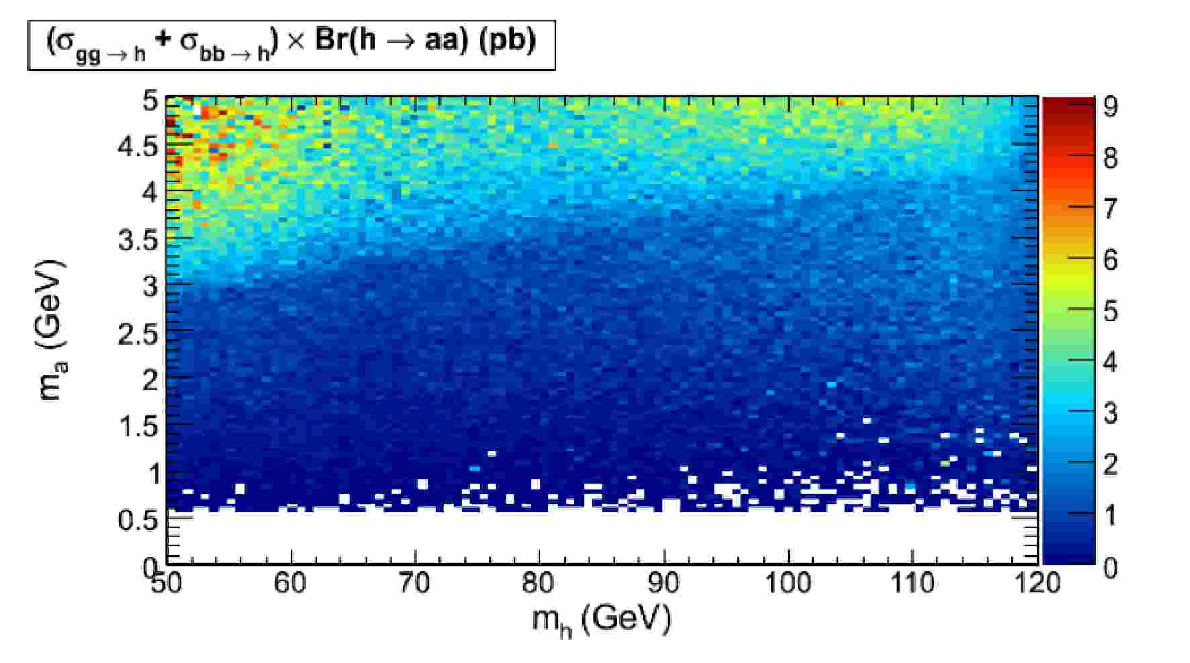
\includegraphics[width=0.5\linewidth]{plots/cs1.eps}%
%% 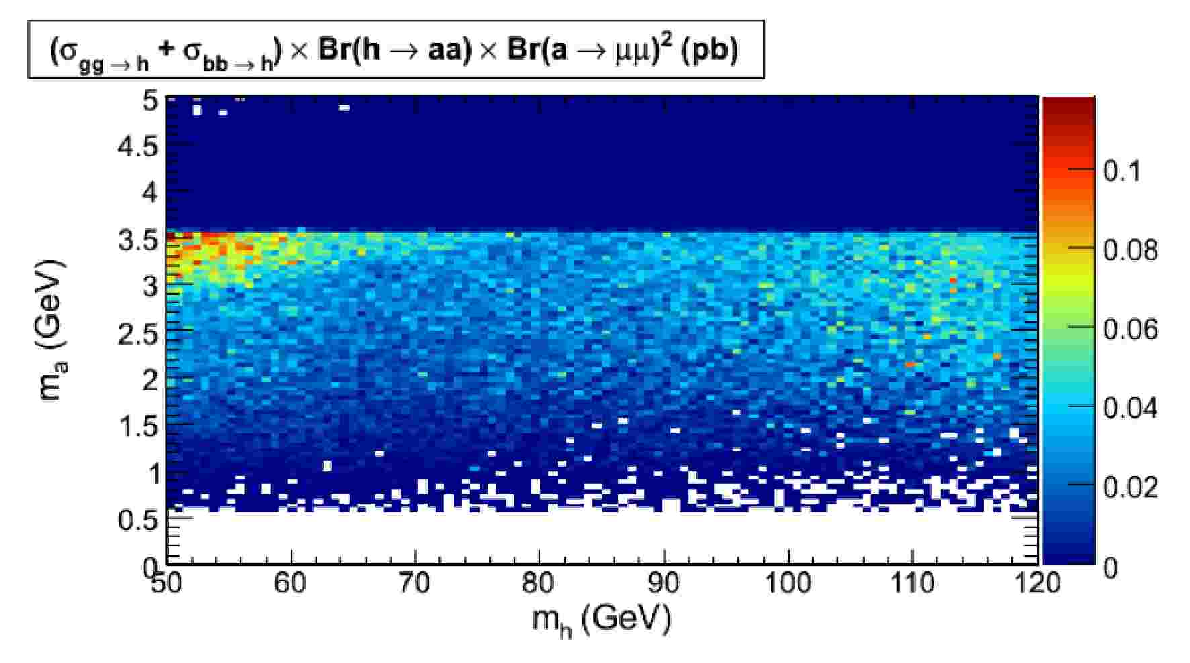
\includegraphics[width=0.5\linewidth]{plots/cs2.eps}%
%% \caption{$m_{a1}-m_{h1}$ plane with
%% color map distribution of
%% for $\sigma(gg+b\bar{b}\to h_1)\times Br(h_1\to a_1 a_1)$ (left) 
%% and $\sigma(gg+b\bar{b}\to h_1)\times Br(h_1\to a_1 a_1)
%% \times Br(a_1\to \mu\mu)^2$ (right) rates.
%% \label{cs2}}
%% \end{figure*}
%% \begin{figure*}[h]
%% 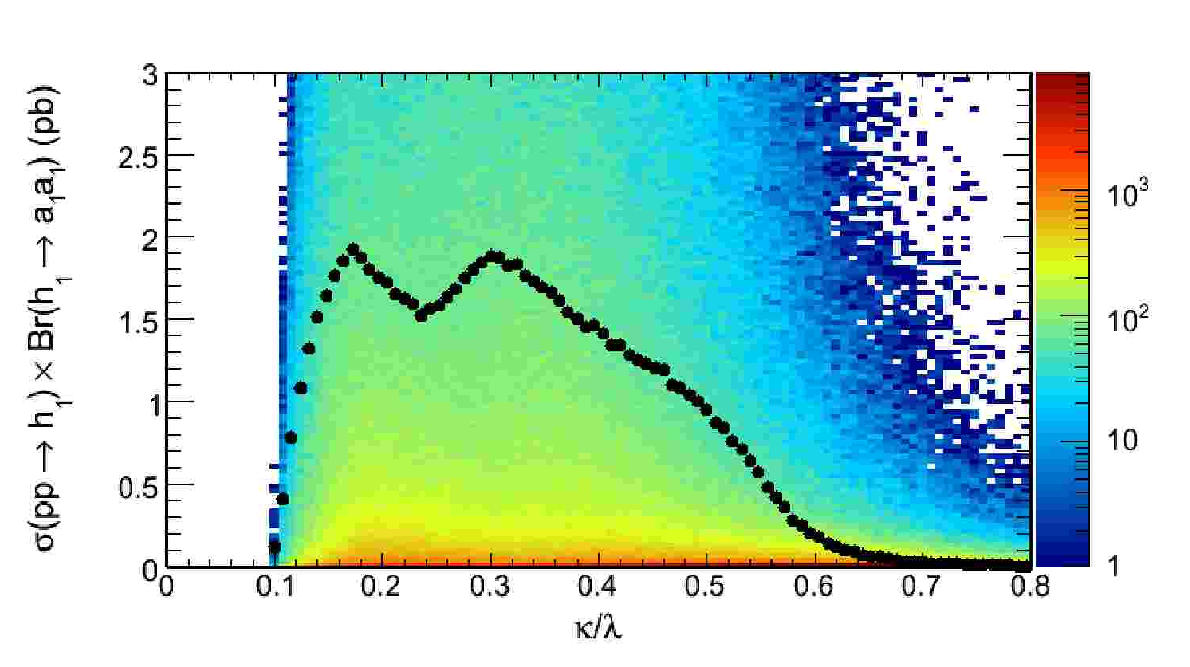
\includegraphics[width=0.5\linewidth]{plots/sig-brh2a_vs_kaplam.eps}%
%% 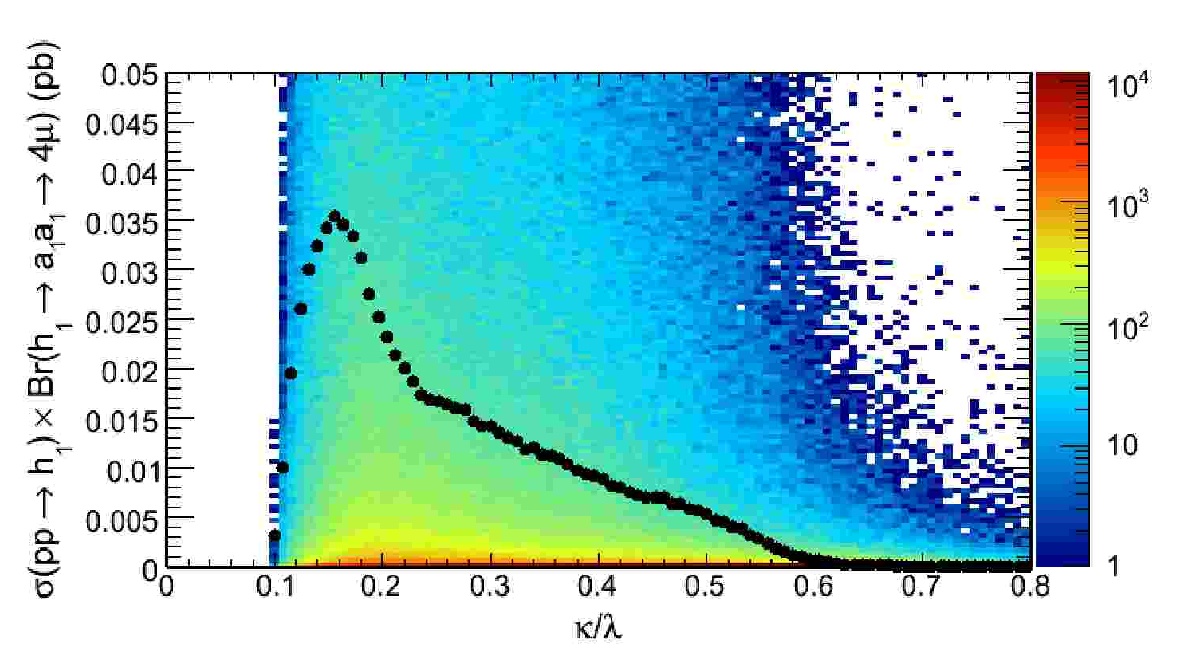
\includegraphics[width=0.5\linewidth]{plots/sig-brh2a-bra2mu_vs_kaplam.eps}%
%% \caption{
%% Distribution of
%% $\sigma(gg+b\bar{b}\to h_1)\times Br(h_1\to a_1 a_1)$ (left)
%% and 
%% $\sigma(gg+b\bar{b}\to h_1)\times Br(h_1\to a_1 a_1)
%% \times Br(a_1\to \mu\mu)^2$ (right) (right)
%% rates
%% versus  $\kappa/\lambda$.
%% \label{sig-brh2a_vs_kaplam}}
%% \end{figure*}

%% In Fig.\ref{cs2} we present $m_{a1}-m_{h1}$ plane with
%% color map distribution of
%% for $\sigma(gg+b\bar{b}\to h_1)\times Br(h_1\to a_1 a_1)$ (left) 
%% and $\sigma(gg+b\bar{b}\to h_1)\times Br(h_1\to a_1 a_1)
%% \times Br(a_1\to \mu\mu)^2$ (right) rates. One can see that
%% $\sigma(gg+b\bar{b}\to h_1)\times Br(h_1\to a_1 a_1)$
%% rate can be quite large and reach about 10 pb for the light $m_{h1}$
%% with the mass about 50 GeV.
%% In the same time,
%% the final cross section of the process under study ---
%% $\sigma(gg+b\bar{b}\to h_1)\times Br(h_1\to a_1 a_1)
%% \times Br(a_1\to \mu\mu)^2 \equiv 
%% \sigma(gg+b\bar{b}\to h_1 \to a_1 a_1 \to 4\mu)$ ---
%% can be only as large as about 0.1 pb.
%% In Fig.\ref{sig-brh2a_vs_kaplam}
%% we present details on the distribution of
%% $\sigma(gg+b\bar{b}\to h_1)\times Br(h_1\to a_1 a_1)$ (left)
%% and 
%% $\sigma(gg+b\bar{b}\to h_1)\times Br(h_1\to a_1 a_1)
%% \times Br(a_1\to \mu\mu)^2$ (right) (right)
%% rates
%% versus  $\kappa/\lambda$.


%% Even though the four-muon signal rates from NMSSM are not high,
%% due to relatively low expected backgrounds the signature of our interest
%% would allow us to exclude significant portion of NMSSM parameter space 
%% even  at low integrated luminosities as we present below.

%% The parameter space accessible at the LHC at low and later on at high luminosity regime
%% is quite unique since it can not be excluded
%% by present low-energy experiments on rare B-meson decays since, as we have found
%% the singlet component of the lightest CP-odd Higgs boson, $a_1$,
%% is extremely close to unity.
%% ({\bf Please  add here reference to the  paper and the talks!}).
%% \\
%% \\
%% ({\bf We should note that of course Tevatron is quite competitve with LHC
%% on the search of $4\mu$ signature from NMSSM since
%% the production corss section at Tevatron is quite large.
%% This is related to the fact that we study the system with comparatively small
%% invariant mass which is not suppressed by gluon parton density
%% since x-values are not large.
%% On the other hand we should present a full potential of the LHC
%% on covering the parameter space of $4\mu$ signature from NMSSM 
%% down to high luminosity and compare Tevatron and LHC potentials
%% in the Figure below.})
%% \begin{figure*}[h]
%% 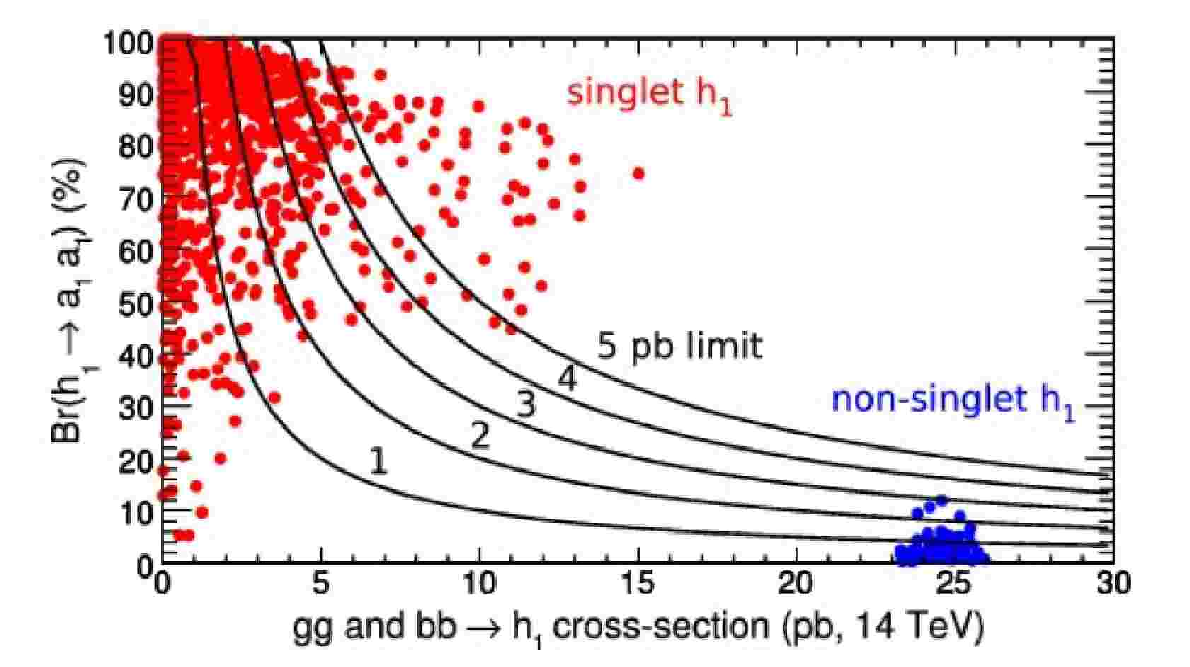
\includegraphics[width=0.5\linewidth]{plots/br_vs_cs.eps}%
%% \caption{
%% \label{}}
%% \end{figure*}
%% ({\bf Another point we should probably explore is to add 
%%      $h2\to h_1 h_1 \to a_1 a_1 + X$ signature. Let me know if you need input from me on this
%%      subject. We have all ingredients for the production rate, so we can easily add this cahnnel.
%%      We can add it in this section or later on.
%%      })
     
\subsection{Summary}
Existing data provides only partial constraints. Requirement of the model consistency with cosmoogical
data leads to XXX. Tevatron data allows constraining of the surviving fraction of the paramater space, 
but only weakly. Further exploration of this region cannot be done at Tevatron b/c that would require
a very significant increase in the size of the datasets. Conclusive exclusion or discovery of new physics
in this scenario would require a dedicated analysis performed at LHC. In the following, we describe such
analysis and discuss its sensitivity.


\section{Dedicated Search for NMSSM at LHC}

The main characteristic of the signal is two back-to-back di-muon pairs with pair consisting of 
spatially close muons. The di-muon pairs should have invariant masses consistent with each other, 
which also allows a direct measurement of $m_a$. Additionally, the four muon invariant mass distribution 
should have a narrow spike corresponding to the $m_h$ mass. We use these striking features of signal 
events in designing the analysis suitable for early LHC running.

The four muon final state considered in this analysis is experimentally a very clean signature 
with relatively low backgrounds. Therefore, instead of using the Vector Boson Fusion (VBF)
chosen in earlier NMSSM searches targeting the $m_a>2 m_\tau$ region, we focus on the largest 
Higgs production modes at the LHC, $gg \to h_1$ and $b\bar{b} \to h_1$.  To calculate NMSSM NLO 
cross-section for $pp \to h_1$ we follow the same procedure (Eqs.~\ref{eq:ggcross_section} and~\ref{eq:bbcross_section})
as for the Tevatron case based on rescaling NLO calculations~\cite{Spira:1995rr,Balazs:1998sb} 
to correct for differences in couplings between SM and NMSSM. Similar to the Tevatron case, the 
cross-section is strongly suppressed compared to SM if $h_1$ 
has a large singlet fraction. Figure~\ref{fig:sm_mukoverl2} shows the production cross-section for 14~TeV $pp \to h_1 X$ 
as a function of $\mu\kappa/\lambda$.  Note that the low $\mu\kappa/\lambda$ and low $\lambda$ 
region is excluded by WMAP, see Fig.~\ref{fig:exclusion}. The non-excluded region have appreciable
production cross-section.

\subsection{Analysis Selections}
We use Pythia to generate signal event templates with $m_h$ in the range from 70 to 140 GeV/c$^2$
and $m_a$  in the range from 0.5 to 4 GeV/c$^2$). For detector response emulation, we chose the CMS 
detector as a benchmark and used its parameters descibed in CMS Technical Design Report. The key 
parameters important for this analysis are muon momentum resolution, low threshold on muons to 
reach the muon system, acceptance and average muon reconstruction efficiencies. 

\begin{figure*}[htbp]
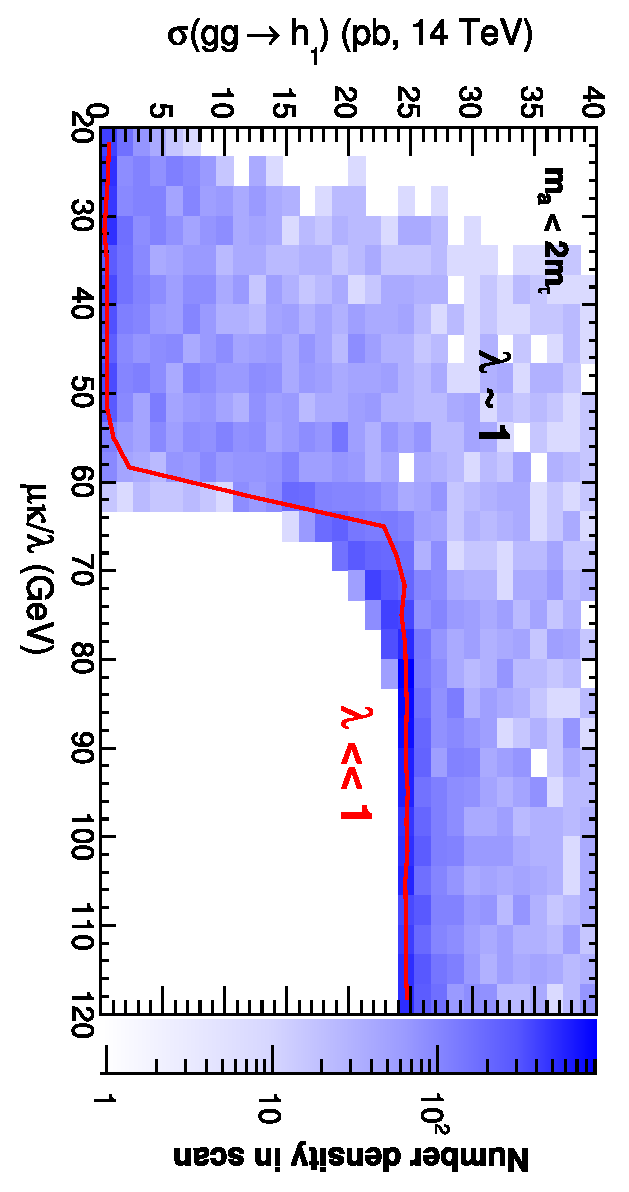
\includegraphics[height=0.48\linewidth, angle=90]{plots/newbranching/crosssec_vs_mukoverl_gg.eps}
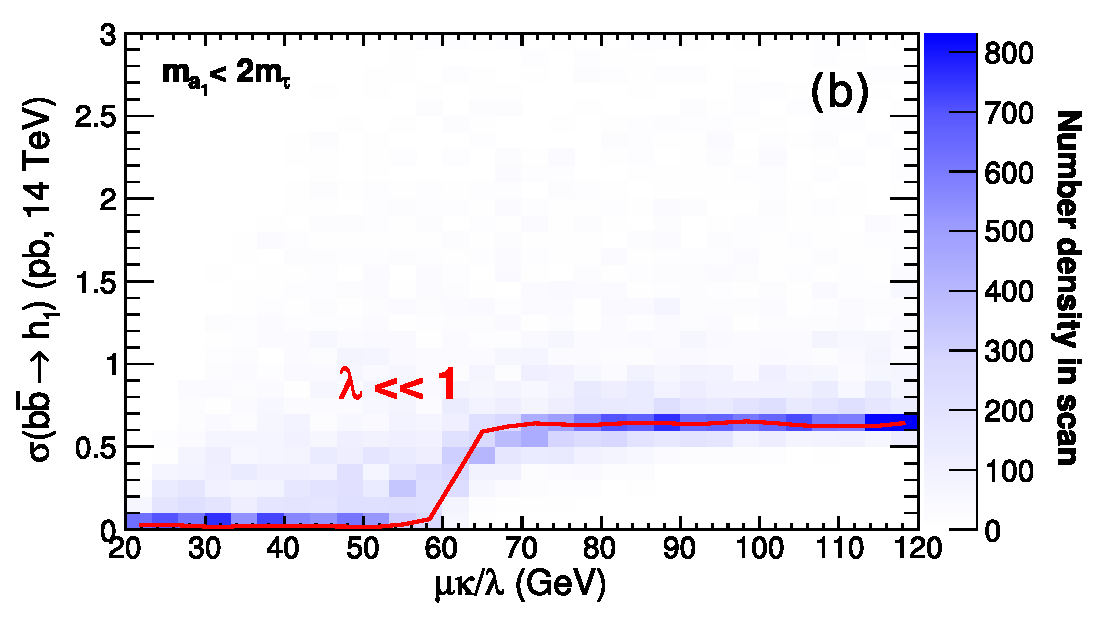
\includegraphics[height=0.48\linewidth, angle=90]{plots/newbranching/crosssec_vs_mukoverl_bb.eps}
%%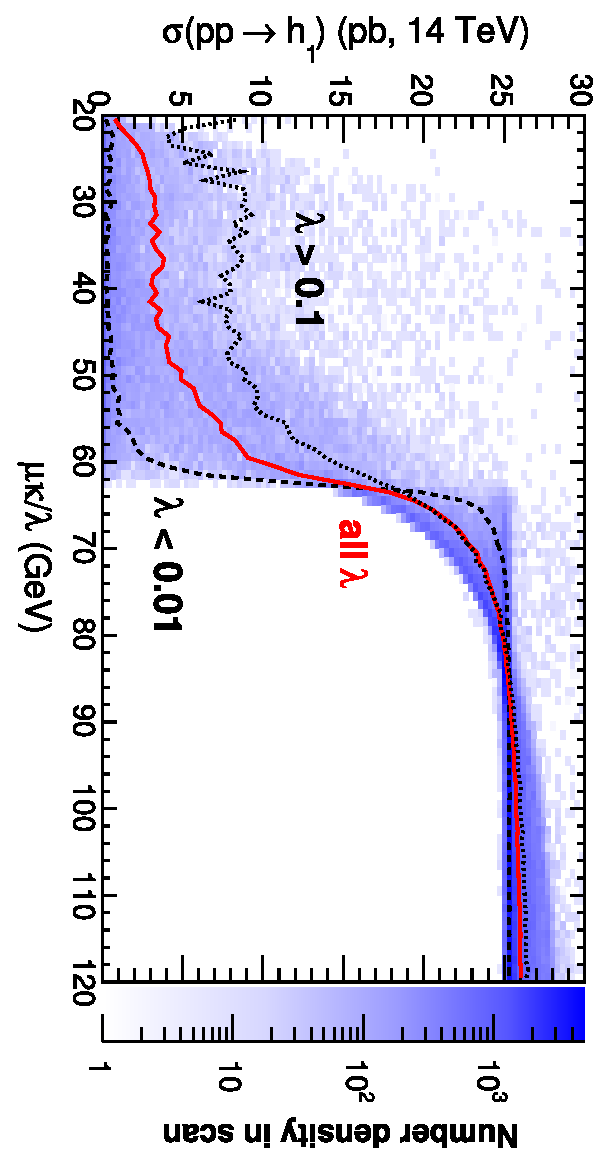
\includegraphics[height=0.7\linewidth, angle=90]{plots/newbranching/crosssec_vs_mukoverl.eps}
\caption{14~TeV production cross-section of $h_1$ as a function of
  $\mu\kappa/\lambda$ and $\lambda$, from $gg$ (left) and $b\bar{b}$
  (right), with the requirement that $m_a < 2m_\tau$.  The red line represents the single-valued $\lambda \ll 1$ limit.
  \label{fig:sm_mukoverl2}}
\end{figure*}


The analysis starts by requiring at least four muon candidates with $p_T>5$ \gevc in the fiducial 
volume of the detector $|\eta|<2.4$, of which at least one has to have $p_T>20$ $\gevc$ to suppress 
major backgrounds and to satisfy trigger requirements. Each event must have at least two muon 
candidates of positive and negative charge each. For surviving events, we define quadruplets of 
candidates consisting of two positive and two negatively charged muon candidates. Next, we sort the 
four muon candidates in quadruplet into two di-muon pairs by minimizing the quantity 
$(\Delta R(\mu_i,\mu_j)^2 + \Delta R (\mu_k,\mu_l)^2)$ under the constarint that each di-muon pair
consists of two muon candidates of opposite charge. Quadruplets in which $\Delta R$ between 
muons in any of the two pair exceeds 0.5 are discarded as inconsistent with signal topology. 
Acceptance of the selections listed above is shown in Fig.~\ref{signal_acceptance} for several
representative choices of values for $m_h$ and $m_a$. 

\begin{figure*}[htbp]
\begin{center}
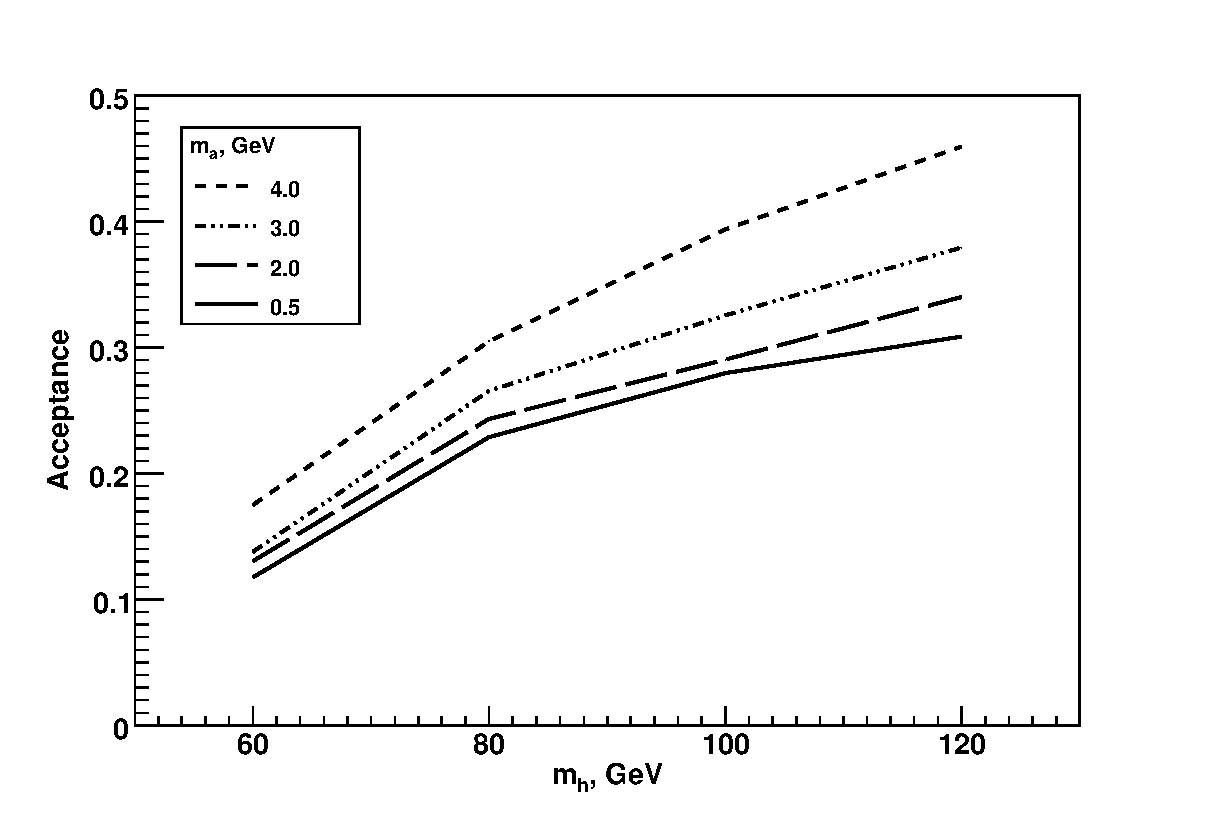
\includegraphics[width=0.48\linewidth]{plots/acceptance_vs_mh.eps}
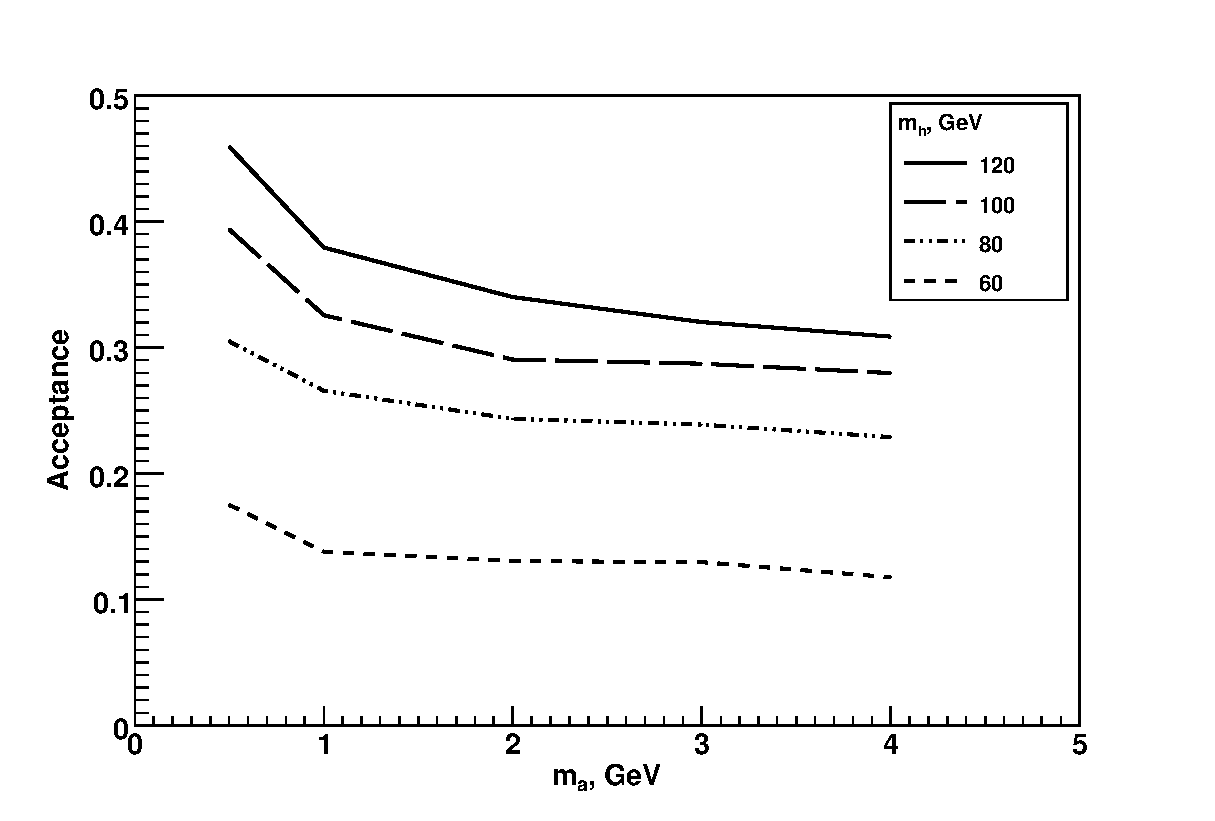
\includegraphics[width=0.48\linewidth]{plots/acceptance_vs_ma.eps}
\caption{Acceptance as a function of $m_a$ for fixed $m_h$. Acceptance as a function of $m_h$ for fixed $m_a$.}
\label{signal_acceptance}
\end{center}
\end{figure*}


Requirement of four sufficiently energetic muons in the event drastically reduces contributions of 
potential backgrounds for this analysis. After acceptance selections, the dominant background is 
due to QCD multijet production where muons originate from either heavy flavor quark decays or from 
$K/\pi$ decays in flight. We use Pythia to estimate the QCD multijet background and we estimate it
at this stage to be approximately 2.6 events/pb$^{-1}$ (approximately half due to true muons and the 
rest from events with both prompt muons and muons from decays in flight). We also considered electroweak 
backgrounds estimated using CompHEP $pp \to 4l+X$ process to be 0.04 events/pb$^{-1}$ and direct J/psi 
production (Pythia), which was found to be completely negligible. Other SM backgrounds (top, W+jets) 
are negligible in the region of interest of this analysis.

The backgrounds are further reduced by applying kinematics requirements consistent
with the expected signal siganture. We calculate invariant mass of each of the di-muon pair, 
$m_{12}$ and $m_{34}$, as well as the invariant mass of all four muons denoted as $M$. Figure 
\ref{muon_pairs_masses_invariant_mass}a) shows the invariant mass of the muon pairs passing 
all selections in signal events for two choices of $m_h$ and $m_a$. Figure \ref{muon_pairs_masses_invariant_mass}b) 
shows the distribution of the invariant mass $M$ of the four muon system for two benchmark points. 
To focus on the region of interest, we require $M>60$ \gevcc, $m_{12} < 4$, $m_{34} < 4$, which
reduces QCD background to 0.4 events/pb$^{-1}$. 

\begin{figure*}[htb]
\begin{center}
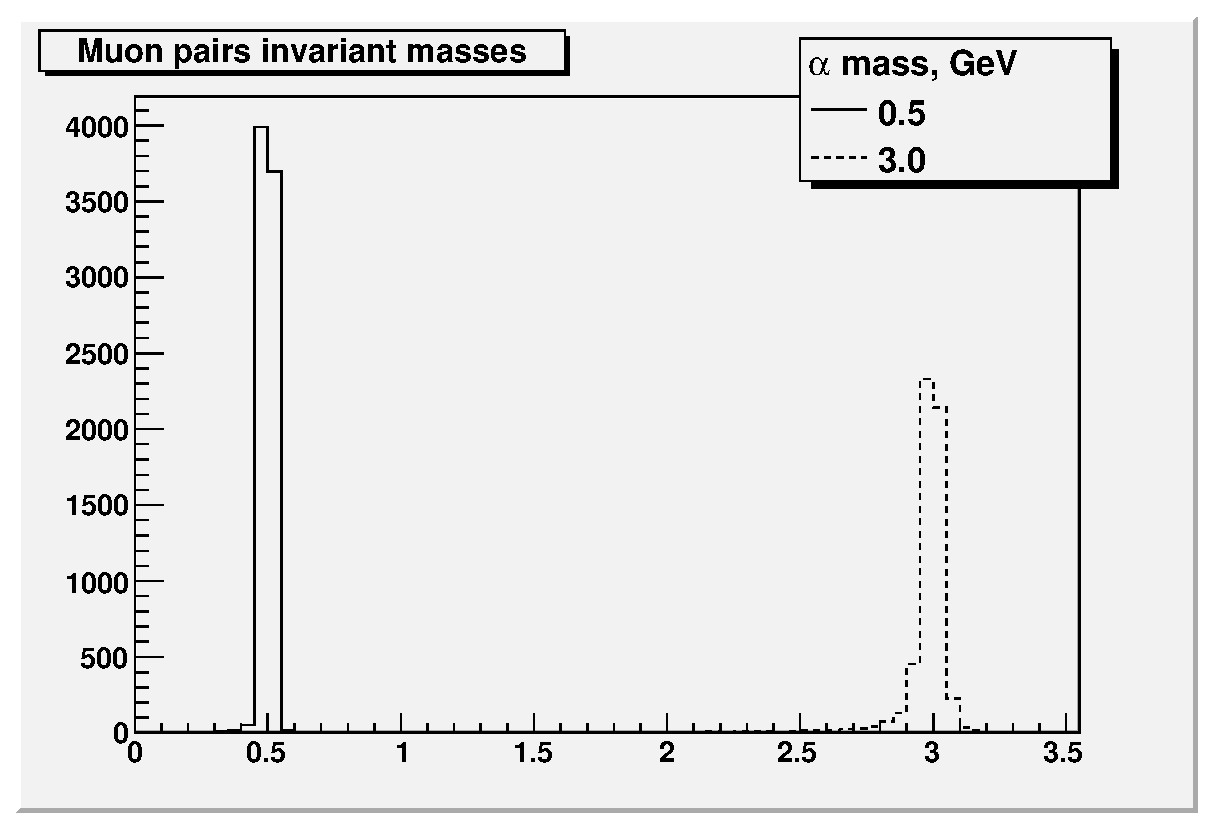
\includegraphics[width=0.48\linewidth]{plots/muon_pairs_masses.eps}
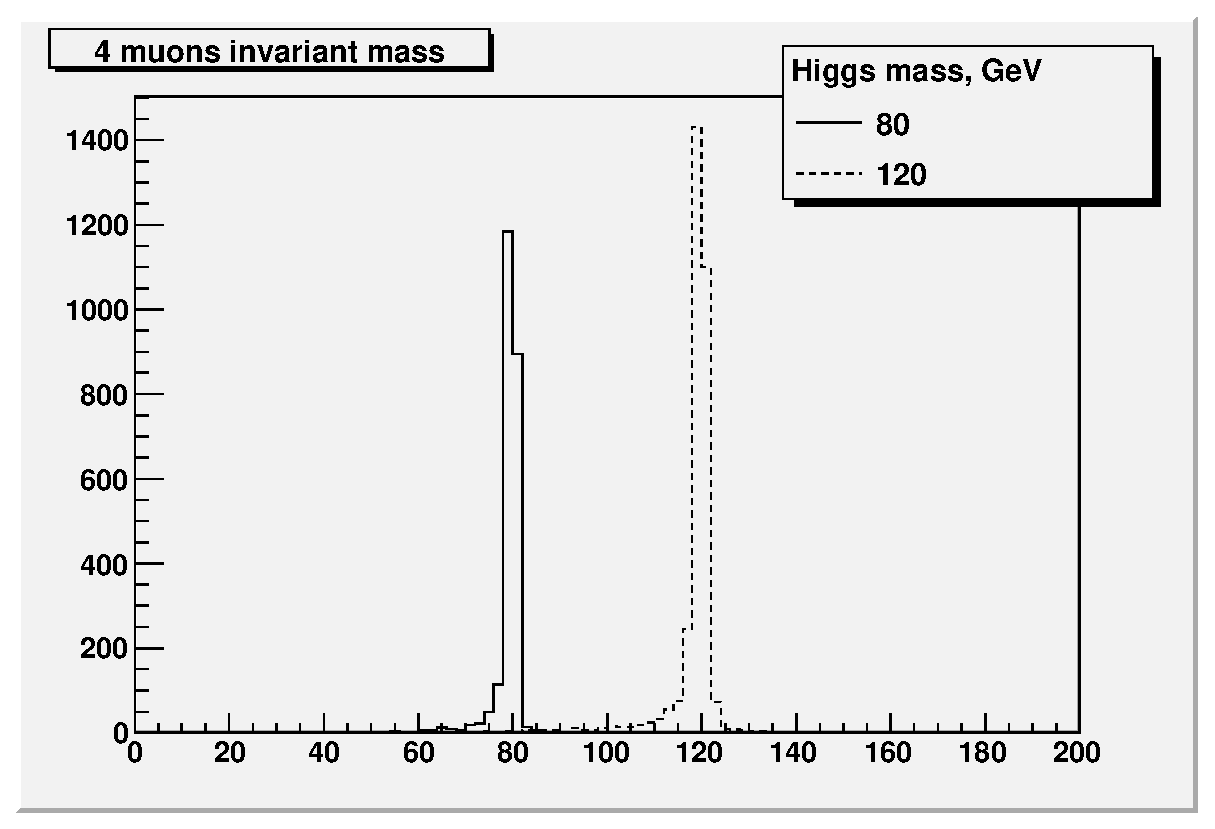
\includegraphics[width=0.48\linewidth]{plots/invariant_mass.eps}
\caption{Left: Reconstructed invariant mass of reconstructed muon pairs for $m_a=0.5$ and 
3 GeV/c$^2$ (in both cases $m_H$ = 100 GeV/c$^2$). Right: Reconstructed invariant of four muons for 
$m_H=80$ and $m_H=120$ GeV/c$^2$ (in both cases $m_a$ = 3.0 GeV).}
\label{muon_pairs_masses_invariant_mass}
\end{center}
\end{figure*}

To ensure the compatibility of the measured invariant masses of two di-muon pairs, one could apply 
a simple cut $|m_{12}-m_{34}|<0.08+0.005*(m_{12}+m_{34})$.  This cut would
enforce the requirement that the two pair masses are consistent with each other and 
it takes into account widening of the absolute resolution in the reconstructed di-muon
mass as a function of mass. If applied, the only background that still may be not completely 
negligible is QCD multi-jet, for which we conservatively estimate the upper bound to be 0.02 
events/pb$^{-1}$. However, instead of applying this selection explicitly, a better approach would 
be to fit the data in the 3D space of 
measured values of $(m_{12},m_{34}, m_{1234})$ taking into account
kinematical properties of  signal events. This approach allows maximizing signal
acceptance and therefore statistical power of the analysis. It is also convenient from 
experimental point of view as the backgrounds
will  be distributed in some smooth fashion over the 3D space allowing fitting the 3D
distribution to estimate  backgrounds directly from the data. Potential signal would
appear as a concentration of events in one specific  region in the 3D space (a 3D
``bump''). We use a binned likelihood defined as a function of parameters $m_a$, 
$m_h$ and effective signal cross section $\sigma \times B (h \to aa) B^2(a \to \mu \mu)$. 
Thus defined likelihood is used to fit pseudodata generated using either background or 
signal+background templates. We estimate sensitivity of the proposed analysis and present 
it in terms of the 95\% C.L. exclusion levels for signal cross-section using Bayesian 
technique.

If necessary, further large background suppression can be obtained by adding the isolation requirement 
to one or both di-muon pairs in the event, e.g. by setting the upper bound on the sum of transverse momenta 
of all tracks in a cone around the reconstructed direction of the di-muon pair excluding momenta of the 
two muon tracks. Such requirement can allow a very substantial suppression of the dominant source of the background coming from events with one or more 
muons originating from jets. We choose not to use this critirea as our estimates show that the final rate 
of such background events is already very low. If data shows larger contribution of these events, 
this isolation requirement would allow bringing backgrounds back to very low level at a moderate
cost to signal acceptance.


%\begin{figure*}[htb]
%\begin{center}
%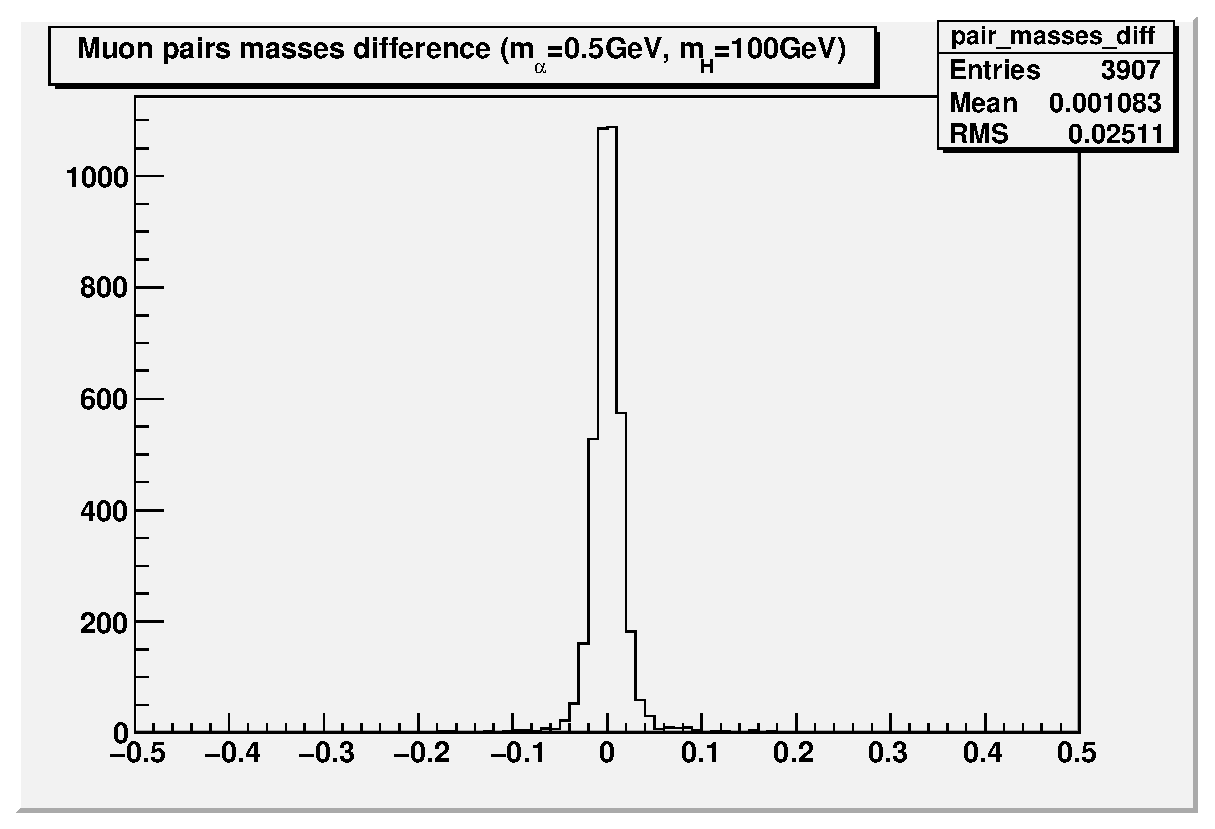
\includegraphics[width=0.48\linewidth]{plots/pairs_masses_diff_0.5.eps}
%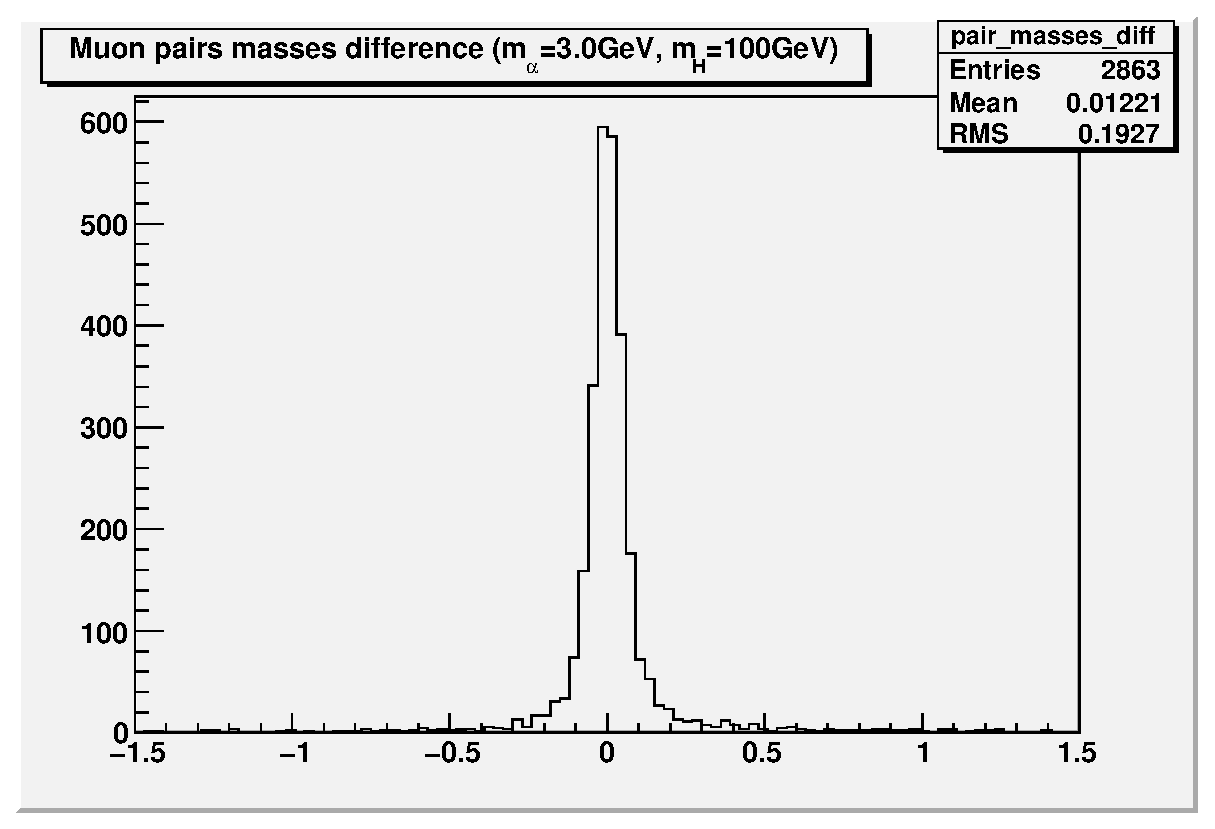
\includegraphics[width=0.48\linewidth]{plots/pairs_masses_diff_3.0.eps}
%\caption{Left: Muon pairs masses difference ($m_a$=0.5GeV, $m_H$=100 GeV). 
%Right: Muon pairs masses difference ($m_a$=3.0GeV, $m_H$=100 GeV)}
%\label{muon_pairs_masses_diff}
%\end{center}
%\end{figure*}


\begin{table}[t]
\caption{Expected number of background events per 100 $\ipb$ of luminosity after selection cuts.\label{bckgr_cuts_number_reco_level}}
\begin{center}
\begin{tabular}{|c|c|c|}
\hline
%\multicolumn{3}{|c|}{hey}\\ \hline
Selections & 4 leptons & QCD multi-jet \\ 
\hline
$p_T (\mu_1)>20$ \gevc \&     &                               &                         \\
$p_T (\mu_i)>5$ \gevc i=2,3,4 &               $4.8\pm0.2$     &    $267\pm23$         \\ 
\hline
$m_{12},m_{34}<4$ \gevcc &           $0.024\pm0.012$ &    $90\pm13$           \\ 
$m_{1234}>60$ \gevcc &           $0.010\pm0.007$ &    $39\pm9$               \\ 
$|m_{12}-m_{34}|< 0.08$ GeV  &&\\       
$+0.005*(m_{12}+m_{34})$ &  $0.000^{+0.005}_{-0.000}$ & {\bf $0.00^{+1.95}_{-0.00}$ }     \\ 
\hline
\end{tabular}
\end{center}
\end{table}

\subsection{Results}
We calculate the 95\% C.L.\ upper limit on the product $\sigma(pp \to h) B_{h \to aa} B^2_{a \to \mu \mu} \, \alpha$, 
using Bayesian technique which is 0.0293~pb at $L = 100$~pb$^{-1}$, approximately 3 events.  In vast majority of 
pseudoexperiments, this limit is independent of $m_h$ and $m_a$ because the effective signal region that dominates 
signal significance in the fitter is essentially background free and probability to observe any pseudodata event is 
very small. The upper limit on $\sigma(pp \to h) B_{h \to aa}$ is shown as a function of $m_h$ and $m_a$ in Table~\ref{table_both_factorized}.  Note that 
$B_{h \to aa}$ is close to 100\% in much of the selected region of NMSSM parameter space.

%\begin{table}[htb]
%\caption{95\% C.L.\ on $\sigma(pp \to h) B_{h \to aa} \, \alpha$ at $L = 100$~pb$^{-1}$ as a function of $m_a$, from Fig~\ref{fig:bramumu}. \label{table_bramumu_factorized}}
%\begin{center}
%\renewcommand{\arraystretch}{1.1}
%\begin{tabular}{| c | c | c |}
%\hline
%\mbox{\hspace{0.25 cm}}$m_a$ (GeV)\mbox{\hspace{0.25 cm}} & \mbox{\hspace{0.25 cm}}$B_{a \to \mu\mu}$ (\%)\mbox{\hspace{0.25 cm}} & \mbox{\hspace{0.25 cm}}$\sigma(pp \to h) %B_{h \to aa} \, \alpha$ (pb)\mbox{\hspace{0.25 cm}} \\\hline
%0.5 & 0 & $\infty$ \\
%0.75 & 4.2 & 16.5 \\
%1.0 & 10.0 & 2.9 \\
%1.5 & 15.7 & 1.2 \\
%2.0 & 17.2 & 1.0 \\
%2.5 & 17.1 & 1.0 \\
%3.0 & 16.1 & 1.1 \\
%3.5 & 14.8 & 1.3 \\
%3.75 & 1.02 & 282 \\
%4.0 & 0.73 & 557 \\
%5.0 & 0.49 & 1220 \\\hline
%\end{tabular}
%\end{center}
%\end{table}

\begin{table}[htbp]
\caption{95\% C.L.\ upper limit on $\sigma(pp \to h) B_{h \to aa}$ (pb) at $L = 100$~pb$^{-1}$ at the LHC. Variations in $\sigma_{\mbox{95\%}}$ as a function of $m_a$ driven by dependency of $B_{a\to\mu\mu}$ on $m_a$, while tightening of the limit towards higher $m_h$ is due to increase in acceptance with $m_h$. {\bf We need to add a second set of numbers for 1 ifb, but if backgrounds are too big we need to add isolation or at least some educated guess on how isolation will affect backgrounds and signal.} \label{table_both_factorized}}
\begin{center}
\renewcommand{\arraystretch}{1.3}
\begin{tabular}{| c | c | c | c | c | c |}
\hline
\mbox{\hspace{0.25 cm}}$m_h$, $m_a$ (GeV)\mbox{\hspace{0.25 cm}} & \mbox{\hspace{0.25 cm}}0.5\mbox{\hspace{0.25 cm}} & \mbox{\hspace{0.25 cm}}1.0\mbox{\hspace{0.25 cm}} & \mbox{\hspace{0.25 cm}}2.0\mbox{\hspace{0.25 cm}} & \mbox{\hspace{0.25 cm}}3.0\mbox{\hspace{0.25 cm}} & \mbox{\hspace{0.25 cm}}4.0\mbox{\hspace{0.25 cm}} \\\hline
80 & $\infty$ & 10.9 & 4.1 & 4.6 & 2400 \\\hline
100 & $\infty$ & 8.9 & 3.4 & 3.8 & 2000 \\\hline
120 & $\infty$ & 7.7 & 2.9 & 3.4 & 1800 \\\hline
\end{tabular}
\end{center}
\end{table}

%\begin{figure*}[htb]
%\begin{center}
%\includegraphics[width=0.48\linewidth]{plots/likelihood_NoSignal.eps}
%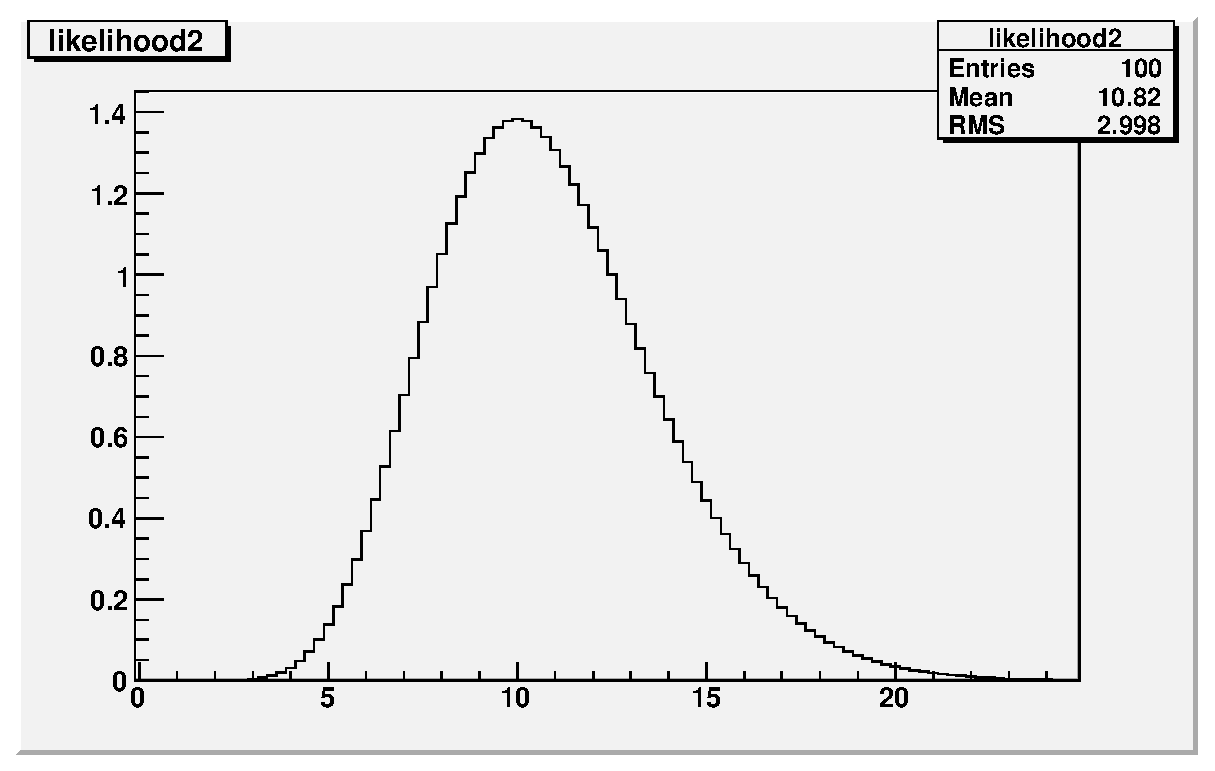
\includegraphics[width=0.48\linewidth]{plots/likelihood_H100_a3_10pb.eps}
%\caption{Left:Example likelihood for a pseudoexperiment for a search assuming $B(H \to aa \to \mu \mu \mu \mu)$=0.04, 
%$m_a=3$ GeV, $m_h= 100$ GeV with null signal shows that a 95\% exclusion is somewhere around 2.5 pb for  
%$\sigma (pp \to H)$. Right: Example likelihood for $\sigma (pp \to H)$=10 \ipb, $B(H \to aa \to \mu \mu \mu \mu)$=0.04, $m_a=3$ GeV 
%$m_h= 100$ GeV shows a more than $5 \sigma$ observation.}
%\label{likelihood_10pb}
%\end{center}
%\end{figure*}

\begin{figure*}[htbp]
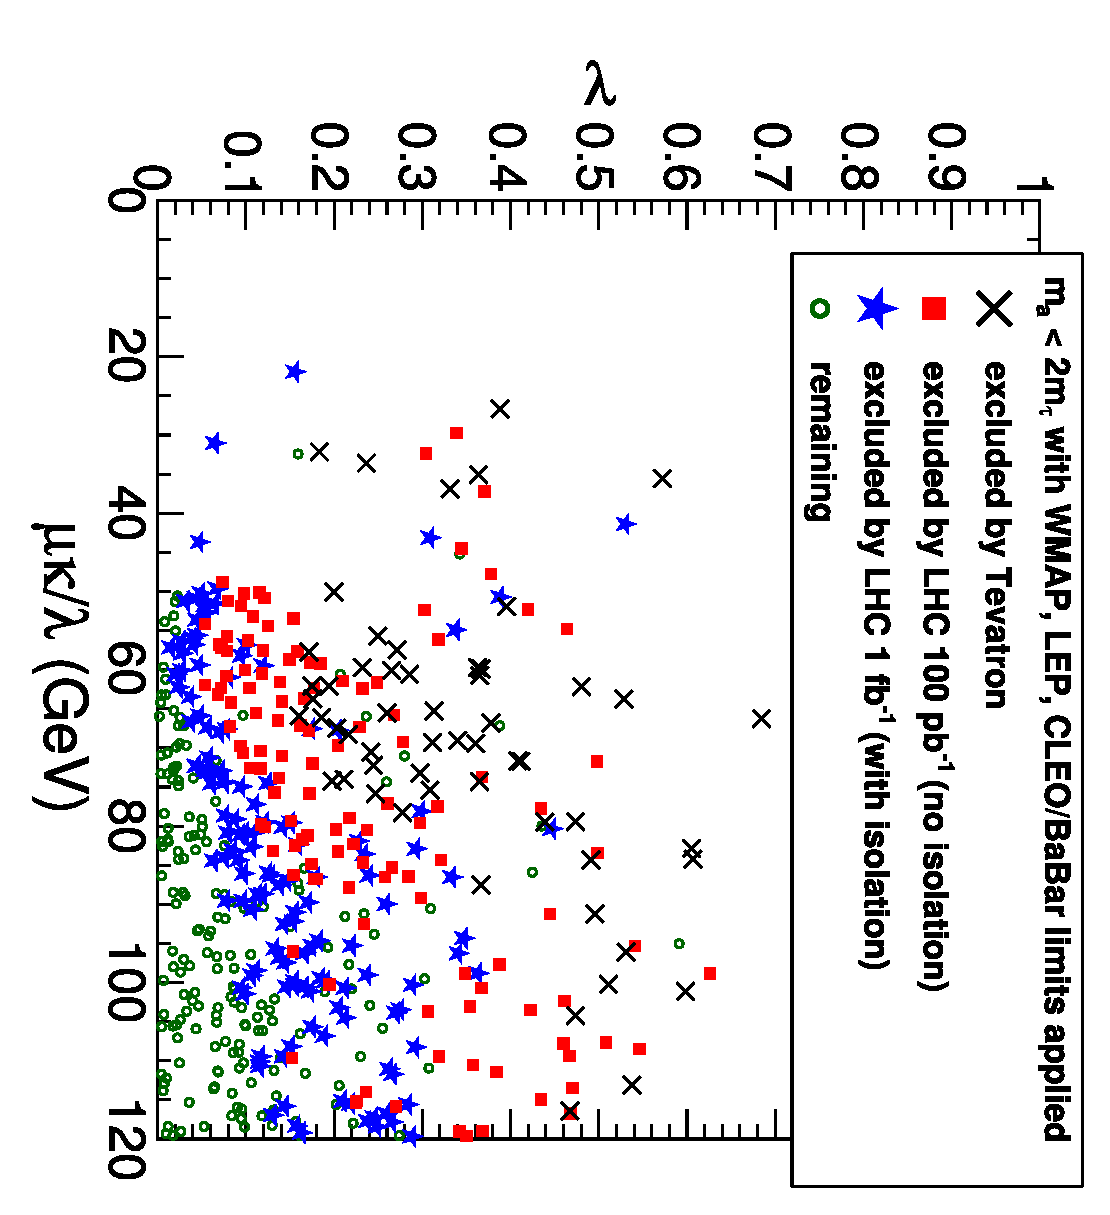
\includegraphics[height=0.32\linewidth, angle=90]{plots/newbranching/newlhcconstraints_params.eps}
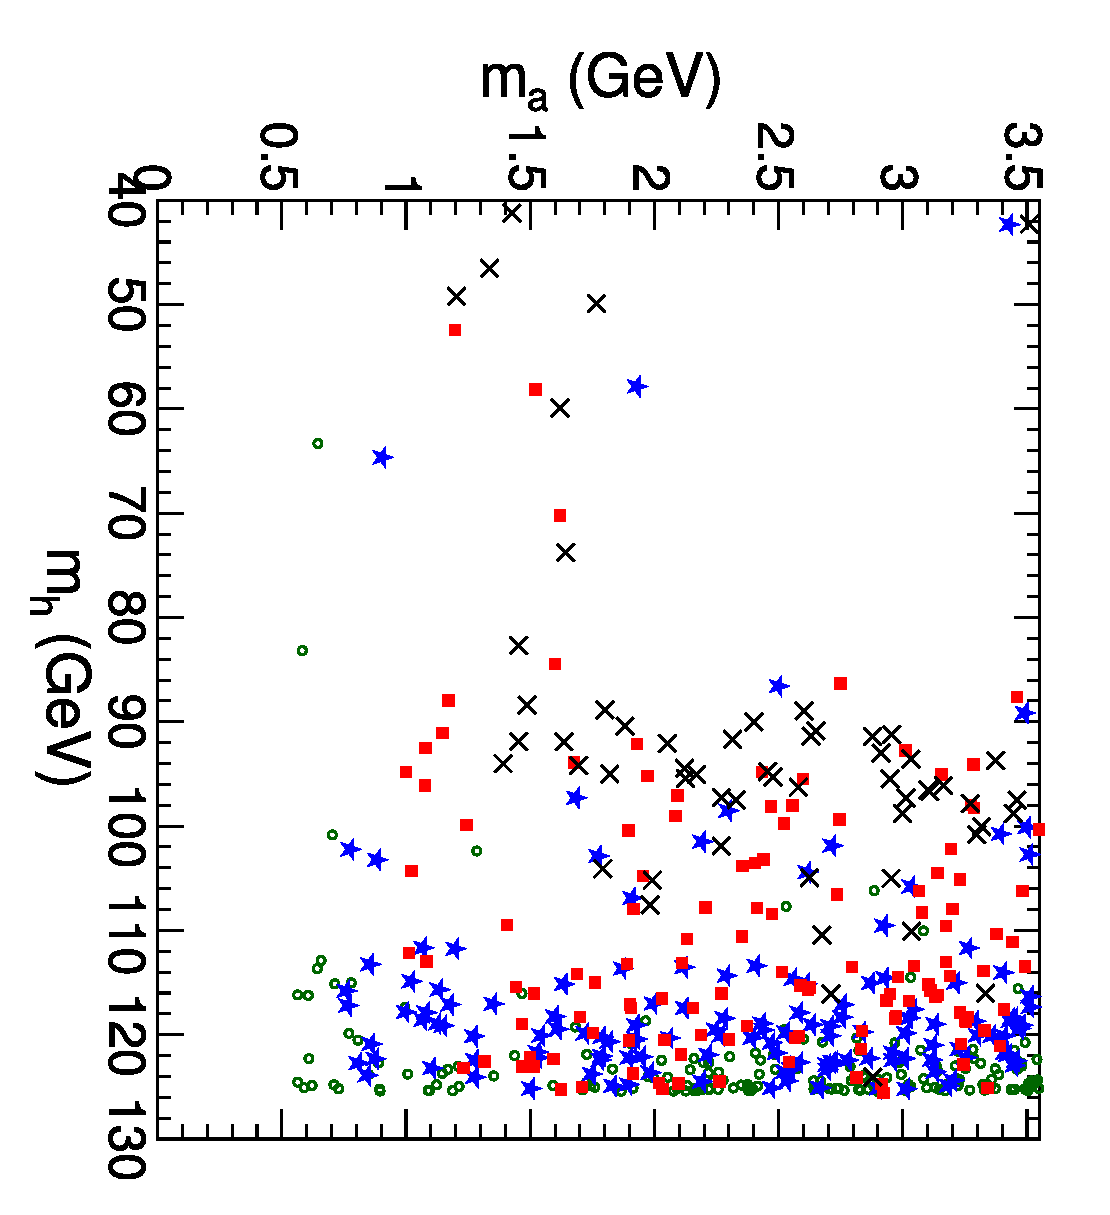
\includegraphics[height=0.32\linewidth, angle=90]{plots/newbranching/newlhcconstraints_masses.eps}
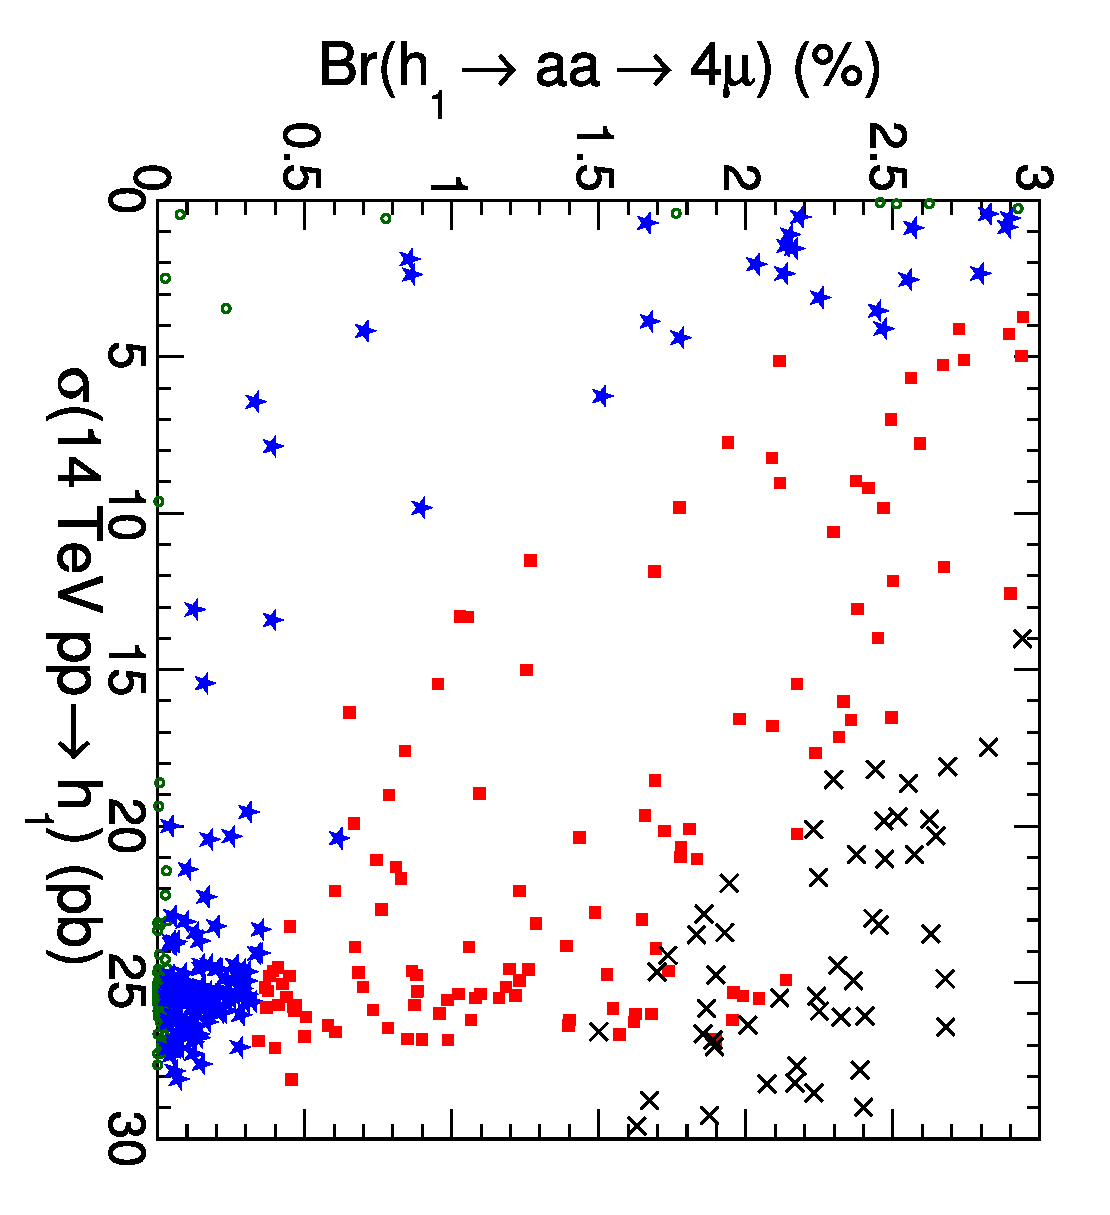
\includegraphics[height=0.32\linewidth, angle=90]{plots/newbranching/newlhcconstraints_crosbr.eps}

\caption{Sampled models excluded by the Tevatron and LHC (with $m_a < 2m_\tau$, WMAP, and LEP constraints applied in all cases).  With only 100~pb$^{-1}$, the LHC's reach extends beyond that of the Tevatron. \label{fig:lhcexclusion}}
\end{figure*}


\section{Results}

{\bf TO BE WRITTEN}

 




%
\section*{Acknowledgments}
We thank 
Ulrich Ellwanger, Cyril Hugonie,
Alexander Pukhov, Jay Wacker
for usefull discussions


%\clearpage
%
%  References
%

%%%%%%%%%%%%%%%%%%%%%%%%%%%% References section %%%%%%%%%%%%%%%%%%%%%%%%%%
% A useful Journal macro
\def\Journal#1#2#3#4{{#1} {\bf #2}, #3 (#4)}
% Some useful journal names
\def\NCA{Nuovo Cimento}
\def\NIM{Nucl. Instrum. Methods}
\def\NIMA{{Nucl. Instrum. Methods} A}
\def\NP{Nucl. Phys.} 
\def\NPB{{Nucl. Phys.} B}
\def\PLB{{Phys. Lett.}  B}
\def\PRL{Phys. Rev. Lett.}
\def\RPP{Rep. Prog. Phys.}
\def\PRD{{Phys. Rev.} D}
\def\PR{Phys. Rep.}
\def\PRP{Prog. Theor. Phys.}
\def\ZPC{{Z. Phys.} C}
\def\MPL{{Mod. Phys. Lett.} A}
\def\EPJC{{Eur. Phys. J.} C}
\def\CPC{Comput. Phys. Commun.}

\renewcommand{\baselinestretch}{1}
%\mytableorig

\begin{thebibliography}{99}

\bibitem{Nilles:1982dy}
  H.~P.~Nilles, M.~Srednicki and D.~Wyler,
  %``Weak Interaction Breakdown Induced By Supergravity,''
  Phys.\ Lett.\  B {\bf 120} (1983) 346.
  %%CITATION = PHLTA,B120,346;%%

%\cite{Frere:1983ag}
\bibitem{Frere:1983ag}
  J.~M.~Frere, D.~R.~T.~Jones and S.~Raby,
  %``Fermion Masses And Induction Of The Weak Scale By Supergravity,''
  Nucl.\ Phys.\  B {\bf 222} (1983) 11.
  %%CITATION = NUPHA,B222,11;%%


%\cite{Ellis:1988er}
\bibitem{Ellis:1988er}
  J.~R.~Ellis, J.~F.~Gunion, H.~E.~Haber, L.~Roszkowski and F.~Zwirner,
  %``Higgs Bosons in a Nonminimal Supersymmetric Model,''
  Phys.\ Rev.\  D {\bf 39} (1989) 844.
  %%CITATION = PHRVA,D39,844;%%

%\cite{Drees:1988fc}
\bibitem{Drees:1988fc}
  M.~Drees,
  %``Supersymmetric Models with Extended Higgs Sector,''
  Int.\ J.\ Mod.\ Phys.\  A {\bf 4} (1989) 3635.
  %%CITATION = IMPAE,A4,3635;%%

%\cite{Ellwanger:1993hn}
\bibitem{Ellwanger:1993hn}
  U.~Ellwanger,
  % ``Radiative corrections to the neutral Higgs spectrum in
  %supersymmetry with a gauge singlet,''
  Phys.\ Lett.\  B {\bf 303} (1993) 271
  [arXiv:hep-ph/9302224].
  %%CITATION = PHLTA,B303,271;%%

%\cite{Ellwanger:1993xa}
\bibitem{Ellwanger:1993xa}
  U.~Ellwanger, M.~Rausch de Traubenberg and C.~A.~Savoy,
  %``Particle spectrum in supersymmetric models with a gauge singlet,''
  Phys.\ Lett.\  B {\bf 315} (1993) 331
  [arXiv:hep-ph/9307322].
  %%CITATION = PHLTA,B315,331;%%

%\cite{Elliott:1993bs}
\bibitem{Elliott:1993bs}
  T.~Elliott, S.~F.~King and P.~L.~White,
  % ``Radiative corrections to Higgs boson masses in the next-to-minimal
  %supersymmetric Standard Model,''
  Phys.\ Rev.\  D {\bf 49} 2435 (1994) 2435
  [arXiv:hep-ph/9308309].
  %%CITATION = PHRVA,D49,2435;%%

%\cite{Pandita:1993tg}
\bibitem{Pandita:1993tg}
  P.~N.~Pandita,
  % ``Radiative corrections to the scalar Higgs masses in a nonminimal
  %supersymmetric Standard Model,''
  Z.\ Phys.\  C {\bf 59} (1993) 575.
  %%CITATION = ZEPYA,C59,575;%%

%\cite{Ellwanger:1995ru}
\bibitem{Ellwanger:1995ru}
  U.~Ellwanger, M.~Rausch de Traubenberg and C.~A.~Savoy,
  %``Higgs phenomenology of the supersymmetric model with a gauge singlet,''
  Z.\ Phys.\  C {\bf 67} (1995) 665
  [arXiv:hep-ph/9502206].
  %%CITATION = ZEPYA,C67,665;%%

%\cite{King:1995vk}
\bibitem{King:1995vk}
  S.~F.~King and P.~L.~White,
  % ``Resolving the constrained minimal and next-to-minimal supersymmetric
  %standard models,''
  Phys.\ Rev.\  D {\bf 52} (1995) 4183
  [arXiv:hep-ph/9505326].
  %%CITATION = PHRVA,D52,4183;%%

%\cite{Franke:1995tc}
\bibitem{Franke:1995tc}
  F.~Franke and H.~Fraas,
  % ``Neutralinos and Higgs Bosons in the Next-To-Minimal
  % Supersymmetric Standard Model,''
  Int.\ J.\ Mod.\ Phys.\  A {\bf 12} (1997) 479
  [arXiv:hep-ph/9512366].
  %%CITATION = IMPAE,A12,479;%%

%\cite{Ellwanger:1996gw}
\bibitem{Ellwanger:1996gw}
  U.~Ellwanger, M.~Rausch de Traubenberg and C.~A.~Savoy,
  %``Phenomenology of supersymmetric models with a singlet,''
  Nucl.\ Phys.\  B {\bf 492} (1997) 21
  [arXiv:hep-ph/9611251].
  %%CITATION = NUPHA,B492,21;%%


\bibitem{Miller:2003ay}
  D.~J.~Miller, R.~Nevzorov and P.~M.~Zerwas,
  %``The Higgs sector of the next-to-minimal supersymmetric standard model,''
  Nucl.\ Phys.\  B {\bf 681} (2004) 3.
%  [arXiv:hep-ph/0304049].
  %%CITATION = NUPHA,B681,3;%%
  
\bibitem{mu-problem}
J.~E.~Kim and H.~P.~Nilles,
  %``The Mu Problem And The Strong CP Problem,''
  Phys.\ Lett.\  B {\bf 138}, 150 (1984).

\bibitem{Dermisek:2005ar}
  R.~Dermisek and J.~F.~Gunion,
  %``Escaping the large fine tuning and little hierarchy problems in the  next
  %to minimal supersymmetric model and h --> a a decays,''
  Phys.\ Rev.\ Lett.\  {\bf 95}, 041801 (2005)
  [arXiv:hep-ph/0502105].

\bibitem{nmssm-ph1}
B.~A.~Dobrescu, G.~L.~Landsberg and K.~T.~Matchev,
  %``Higgs boson decays to CP-odd scalars at the Tevatron and beyond,''
  Phys.\ Rev.\  D {\bf 63}, 075003 (2001)
  [arXiv:hep-ph/0005308];
%
 B.~A.~Dobrescu and K.~T.~Matchev,
  %``Light axion within the next-to-minimal supersymmetric standard model,''
  JHEP {\bf 0009}, 031 (2000)
  [arXiv:hep-ph/0008192].
  
\bibitem{nmssm-ph2}
 J.~F.~Gunion, H.~E.~Haber and T.~Moroi,
  %``Will at least one of the Higgs bosons of the next-to-minimal
  %supersymmetric extension of the standard model be observable at LEP2  or the
  %LHC?,''
{\it In the Proceedings of 1996 DPF / DPB Summer Study on New Directions for High-Energy Physics (Snowmass 96), Snowmass, Colorado, 25 Jun - 12
Jul 1996, pp LTH095}
  [arXiv:hep-ph/9610337];
  %
  U.~Ellwanger, J.~F.~Gunion and C.~Hugonie,
  %``Establishing a no-lose theorem for NMSSM Higgs boson discovery at the
  %LHC,''
  arXiv:hep-ph/0111179
  
\bibitem{nmssm-ph2b}
   %
 J.~R.~Ellis, J.~F.~Gunion, H.~E.~Haber, L.~Roszkowski and F.~Zwirner,
  %``Higgs Bosons in a Nonminimal Supersymmetric Model,''
  Phys.\ Rev.\  D {\bf 39}, 844 (1989);
  %
  B.~A.~Dobrescu, G.~L.~Landsberg and K.~T.~Matchev,
  %``Higgs boson decays to CP-odd scalars at the Tevatron and beyond,''
  Phys.\ Rev.\  D {\bf 63}, 075003 (2001)
  [arXiv:hep-ph/0005308];
  
    U.~Ellwanger, J.~F.~Gunion, C.~Hugonie and S.~Moretti,
  %``Towards a no-lose theorem for NMSSM Higgs discovery at the LHC,''
  arXiv:hep-ph/0305109;
  %
   %
  U.~Ellwanger, J.~F.~Gunion, C.~Hugonie and S.~Moretti,
  %``NMSSM Higgs discovery at the LHC,''
  %
  arXiv:hep-ph/0401228;
    U.~Ellwanger, J.~F.~Gunion and C.~Hugonie,
  %``Difficult scenarios for NMSSM Higgs discovery at the LHC,''
  JHEP {\bf 0507}, 041 (2005)
  [arXiv:hep-ph/0503203].
  
 
  
\bibitem{nmssm-ph3}
  S.~Moretti, S.~Munir and P.~Poulose,
  %``Another step towards a no-lose theorem for NMSSM Higgs discovery at the
  %LHC,''
  Phys.\ Lett.\  B {\bf 644}, 241 (2007)
  [arXiv:hep-ph/0608233];
  
  
  
\bibitem{nmssm-ph4}
 S.~Chang, P.~J.~Fox and N.~Weiner,
  %``Visible cascade Higgs decays to four photons at hadron colliders,''
  Phys.\ Rev.\ Lett.\  {\bf 98}, 111802 (2007)
  [arXiv:hep-ph/0608310]. 
  
\bibitem{nmssm-ph5}
  R.~Dermisek and J.~F.~Gunion,
  %``The NMSSM close to the R-symmetry limit and naturalness in h --> aa  decays
  %for m(a) < 2m(b),''
  Phys.\ Rev.\  D {\bf 75}, 075019 (2007)
  [arXiv:hep-ph/0611142].  
  
\bibitem{nmssm-ph6}
 K.~Cheung, J.~Song and Q.~S.~Yan,
  %``Role of h --> eta eta in Intermediate-Mass Higgs Boson Searches at the
  %Large Hadron Collider,''
  Phys.\ Rev.\ Lett.\  {\bf 99}, 031801 (2007)
  [arXiv:hep-ph/0703149]. 

\bibitem{nmssm-ph6a}  
  J.~R.~Forshaw, J.~F.~Gunion, L.~Hodgkinson, A.~Papaefstathiou and A.~D.~Pilkington,
  %``Reinstating the 'no-lose' theorem for NMSSM Higgs discovery at the LHC,''
  JHEP {\bf 0804} (2008) 090
  [arXiv:0712.3510 [hep-ph]].  
  
\bibitem{nmssm-ph7}
  A.~Belyaev, S.~Hesselbach, S.~Lehti, S.~Moretti, 
  A.~Nikitenko and C.~H.~Shepherd-Themistocleous,
  %``The Scope of the 4 tau Channel in Higgs-strahlung and Vector Boson Fusion
  %for the NMSSM No-Lose Theorem at the LHC,''
  arXiv:0805.3505 [hep-ph]. 
  
\bibitem{nmssm-dm}
A.~Menon, D.~E.~Morrissey and C.~E.~M.~Wagner,
  %``Electroweak baryogenesis and dark matter in the nMSSM,''
  Phys.\ Rev.\  D {\bf 70} (2004) 035005
  [arXiv:hep-ph/0404184];
  D.~G.~Cerdeno, C.~Hugonie, D.~E.~Lopez-Fogliani, C.~Munoz and A.~M.~Teixeira,
  %``Theoretical predictions for the direct detection of neutralino dark  matter
  %in the NMSSM,''
  JHEP {\bf 0412} (2004) 048
  [arXiv:hep-ph/0408102];
  %
  G.~Belanger, F.~Boudjema, C.~Hugonie, A.~Pukhov and A.~Semenov,
  %``Relic density of dark matter in the NMSSM,''
  JCAP {\bf 0509}, 001 (2005)
  [arXiv:hep-ph/0505142];
  %
  J.~F.~Gunion, D.~Hooper and B.~McElrath,
  %``Light neutralino dark matter in the NMSSM,''
  Phys.\ Rev.\  D {\bf 73}, 015011 (2006)
  [arXiv:hep-ph/0509024];
  %
  F.~Ferrer, L.~M.~Krauss and S.~Profumo,
  %``Indirect detection of light neutralino dark matter in the NMSSM,''
  Phys.\ Rev.\  D {\bf 74}, 115007 (2006)
  [arXiv:hep-ph/0609257];
  %
   D.~G.~Cerdeno, E.~Gabrielli, D.~E.~Lopez-Fogliani, C.~Munoz and A.~M.~Teixeira,
  %``Phenomenological viability of neutralino dark matter in the NMSSM,''
  JCAP {\bf 0706}, 008 (2007)
  [arXiv:hep-ph/0701271];
  %
  C.~Hugonie, G.~Belanger and A.~Pukhov,
  %``Dark Matter in the Constrained NMSSM,''
  JCAP {\bf 0711}, 009 (2007)
  [arXiv:0707.0628 [hep-ph]];
  %
  V.~Barger, P.~Langacker, I.~Lewis, M.~McCaskey, G.~Shaughnessy and B.~Yencho,
  %``Recoil detection of the lightest neutralino in MSSM singlet extensions,''
  Phys.\ Rev.\  D {\bf 75}, 115002 (2007)
  [arXiv:hep-ph/0702036].
  %
  S.~Kraml, A.~R.~Raklev and M.~J.~White,
  %``NMSSM in disguise: discovering singlino dark matter with soft leptons at
  %the LHC,''
  Phys.\ Lett.\  B {\bf 672}, 361 (2009)
  [arXiv:0811.0011 [hep-ph]];
  %
  G.~Belanger, C.~Hugonie and A.~Pukhov,
  %``Precision measurements, dark matter direct detection and LHC Higgs searches
  %in a constrained NMSSM,''
  JCAP {\bf 0901}, 023 (2009)
  [arXiv:0811.3224 [hep-ph]].
  


\bibitem{nmssmtools1} U.~Ellwanger, J.F.~Gunion and C.~Hugoine,
\Journal{JHEP}{0502}{066}{2005}.

\bibitem{nmssmtools2} U.~Ellwanger, C.~Hugoine, \Journal{\CPC}{175}{290}{2006}.

\bibitem{nmssmtools3} F.~Domingo and U.~Ellwanger, arXiv:0710.3714 [hep-ph].

\bibitem{wmap}
  D.~N.~Spergel {\it et al.}  [WMAP Collaboration],
  %``First Year Wilkinson Microwave Anisotropy Probe (WMAP) Observations:
  %Determination of Cosmological Parameters,''
  Astrophys.\ J.\ Suppl.\  {\bf 148}, 175 (2003)
  [arXiv:astro-ph/0302209];
%
  C.~L.~Bennett {\it et al.}  [WMAP Collaboration],
  %``First Year Wilkinson Microwave Anisotropy Probe (WMAP) Observations:
  %Preliminary Maps and Basic Results,''
  Astrophys.\ J.\ Suppl.\  {\bf 148}, 1 (2003)
  [arXiv:astro-ph/0302207];
%
  D.~N.~Spergel {\it et al.}  [WMAP Collaboration],
  %``Wilkinson Microwave Anisotropy Probe (WMAP) three year results:
  %Implications for cosmology,''
  Astrophys.\ J.\ Suppl.\  {\bf 170}, 377 (2007)
  [arXiv:astro-ph/0603449].  

%\cite{Abazov:2009yi}
\bibitem{Abazov:2009yi}
  V.~M.~Abazov {\it et al.}  [D0 Collaboration],
  %``Search for NMSSM Higgs bosons in the h->aa->mumu mumu, mumu tautau channels
  %using ppbar collisions at sqrt{s}=1.96 TeV,''
  Phys.\ Rev.\ Lett.\  {\bf 103}, 061801 (2009)
  [arXiv:0905.3381 [hep-ex]].
  %%CITATION = PRLTA,103,061801;%%

\bibitem{lep1exclusion} G.~Abbiendi~\etal (OPAL Collaboration),
\Journal{\EPJC}{18}{425-445}{2001}.

\bibitem{lep2exclusion} G.~Abbiendi~\etal (OPAL Collaboration),
\Journal{\EPJC}{27}{483-495}{2003}, arXiv:0209068v1 [hep-ex].

\bibitem{:2008hs}
  W.~Love {\it et al.}  [CLEO Collaboration],
  %``Search for Very Light CP-Odd Higgs Boson in Radiative Decays of
  %Upsilon(S-1),''
  Phys.\ Rev.\ Lett.\  {\bf 101}, 151802 (2008)
  [arXiv:0807.1427 [hep-ex]].
  %%CITATION = PRLTA,101,151802;%%

\bibitem{Aubert:2009cp}
  B.~Aubert {\it et al.}  [BABAR Collaboration],
  %``Search for Dimuon Decays of a Light Scalar Boson in Radiative Transitions
  %Upsilon -> gamma A0,''
  Phys.\ Rev.\ Lett.\  {\bf 103}, 081803 (2009)
  [arXiv:0905.4539 [hep-ex]].
%\cite{Spira:1995rr}

\bibitem{Ellwanger:2009dp}
  U.~Ellwanger, C.~Hugonie and A.~M.~Teixeira,
  %``The Next-to-Minimal Supersymmetric Standard Model,''
  arXiv:0910.1785 [hep-ph].

\bibitem{Spira:1995rr}
  M.~Spira, A.~Djouadi, D.~Graudenz and P.~M.~Zerwas,
  %``Higgs boson production at the LHC,''
  Nucl.\ Phys.\  B {\bf 453}, 17 (1995)
  [arXiv:hep-ph/9504378].
  %%CITATION = NUPHA,B453,17;%%%\cite{Spira:1995mt}

 %\cite{Djouadi:1997yw}
\bibitem{Djouadi:1997yw}
  A.~Djouadi, J.~Kalinowski and M.~Spira,
  %``HDECAY: A program for Higgs boson decays in the standard model and its
  %supersymmetric extension,''
  Comput.\ Phys.\ Commun.\  {\bf 108}, 56 (1998)
  [arXiv:hep-ph/9704448].
  %%CITATION = CPHCB,108,56;%% 

%\cite{Balazs:1998sb}
\bibitem{Balazs:1998sb}
  C.~Balazs, H.~J.~He and C.~P.~Yuan,
  %``QCD corrections to scalar production via heavy quark fusion at hadron
  %colliders,''
  Phys.\ Rev.\  D {\bf 60}, 114001 (1999)
  [arXiv:hep-ph/9812263].
  %%CITATION = PHRVA,D60,114001;%%
  
  
 %\cite{Belyaev:2005nu}
\bibitem{Belyaev:2005nu}
  A.~Belyaev, J.~Pumplin, W.~K.~Tung and C.~P.~Yuan,
  %``Uncertainties of the inclusive Higgs production cross section at the
  %Tevatron and the LHC,''
  JHEP {\bf 0601}, 069 (2006)
  [arXiv:hep-ph/0508222].
  %%CITATION = JHEPA,0601,069;%% 

%\cite{cleo-low-ma}
\bibitem{cleo-low-ma} (CLEO Collaboration) Phys.\ Rev.\ D {\bf 76}, 117102 (2007); 

%\cite{babar-low-ma}
\bibitem{babar-low-ma} (BaBar) Phys. Rev. Lett. 103:081803 (2009);

%\cite{babar-low-ma}
\bibitem{d0-low-ma} PRL 103, 061801 (2009).

%\cite{micrOmegas}
\bibitem{micrOmegas} G. Belanger, F. Boudjema, C. Hugonie, A. Pukhov, A. Semenov, JCAP 0509:001 (2005), arXiv:hep-ph/0505142

  
%
% Coordinate for CDF detector
%

%\bibitem{CDFdet} CDF Collaboration, F.~Abe~\etal, \Journal{\NIMA}{271}{387}{1988}.
    
%\bibitem{Topref} CDF Collaboration, F.~Abe~\etal, \Journal{\PRD}{50}{2966}{1994}.
\end{thebibliography}

\section{Appendix}


\begin{table}[t]
\caption{Background samples normalization\label{bckgr_normalize}}
\begin{center}
\begin{tabular}{|c|c|c|c|c|c|}
\hline
%\multicolumn{3}{|c|}{hey}\\ \hline
Sample & $\sigma$ & $N^{gen}_{evt}$ & Filter efficiency & $L_{eff}$ & $f = L_{100}/L_{eff}$ \\ \hline
$\mu+x$ &           $0.5091mb$    &    $6238383$      &    $0.000239$  &  $51.2709pb^{-1}$   &  $1.9504$ \\ \hline
4 leptons &        $0.538pb$     &    $10995$        &    $1.0$       &  $20436.803pb^{-1}$ &  $0.0049$ \\ \hline
$J/\psi$ &         $0.127.2nb$   &    $1413803$      &    $0.0074$    &  $1502.00pb^{-1}$   &  $0.0666$ \\ \hline

\end{tabular}
\end{center}
\end{table}

\end{document}

\bibitem{Djouadi:2008uw}
  A.~Djouadi {\it et al.},
  %``Benchmark scenarios for the NMSSM,''
  arXiv:0801.4321 [hep-ph].
  %%CITATION = ARXIV:0801.4321;%%

%\cite{Djouadi:2008yj}
\bibitem{Djouadi:2008yj}
  A.~Djouadi, U.~Ellwanger and A.~M.~Teixeira,
  %``The constrained next-to-minimal supersymmetric standard model,''
  arXiv:0803.0253 [hep-ph].
  %%CITATION = ARXIV:0803.0253;%%

\bibitem{cNMSSM-benchmarks} 
A. Djouadi, U. Ellwanger, R. Godbole,  
C. Hugonie,  S.F. King,  S. Lehti, 
S. Moretti, A. Nikitenko, 
I. Rottl\"ander,  M. Schumacher and 
A. M. Teixeira, in arXiv:0803.1154 [hep-ph].
